% !TeX program = xelatex
\documentclass[12pt,a4paper,oneside]{report}
\usepackage{fontspec}
\usepackage[margin=1in]{geometry}
\usepackage{microtype,setspace}
\setstretch{1.22}
\usepackage{amsmath,amssymb,booktabs,array,longtable,tabularx,multirow,graphicx,float,pdflscape}
\usepackage[english]{babel}
\usepackage{csquotes}
\usepackage[backend=biber,style=apa,natbib=true,sortcites=true]{biblatex}
\addbibresource{references.bib}
\usepackage{xcolor,xurl,enumitem,caption,subcaption}
\usepackage[hidelinks,unicode]{hyperref}
% Set \thesisdraftfalse here for a copy without the DRAFT watermark.
\newif\ifthesisdraft
\thesisdrafttrue
\ifthesisdraft
  \AddToHook{shipout/foreground}{%
    \put(.5\paperwidth,-.5\paperheight){%
      \makebox[0pt][c]{\raisebox{-.5\height}{%
        
\includegraphics[width=.70\paperwidth]{figures/draft-watermark.pdf}}}}}
\fi
\captionsetup{labelfont=bf,textfont=it,labelsep=newline,justification=raggedright,singlelinecheck=false,position=top}
\newcommand{\displaynote}[1]{\par\smallskip\begingroup\raggedright\small\noindent\textit{Note.} #1\par\endgroup}
\setlength{\bibhang}{0.5in}
\usepackage{fancyhdr}
\setlength{\headheight}{15pt}
\pagestyle{fancy}\fancyhf{}\fancyhead[L]{\small\nouppercase{\leftmark}}\fancyfoot[C]{\thepage}
\renewcommand{\headrulewidth}{0.3pt}
\setlength{\emergencystretch}{3em}
\setlength{\parskip}{0pt}
\newcommand{\apaprose}{\doublespacing\raggedright\setlength{\parindent}{0.5in}}
\AtBeginEnvironment{longtable}{\singlespacing}
\setcounter{tocdepth}{2}\setcounter{secnumdepth}{2}
\newcolumntype{P}[1]{>{\raggedright\arraybackslash}p{#1}}
\newcolumntype{Y}{>{\raggedright\arraybackslash}X}
% The register is read in the preamble so each URL can be entered literally.
% Keep each EvidenceFile declaration on its own line. A URL may contain a
% percent-encoded path, an underscore, a query string, or a line fragment.
\ExplSyntaxOn
\prop_new:N \g_thesis_evidence_urls_prop
\prop_new:N \g_thesis_evidence_names_prop
\seq_new:N \g_thesis_evidence_rows_seq
\seq_new:N \l_thesis_evidence_note_seq
\NewDocumentCommand{\EvidenceFile}{m m m v}
  {
    \prop_if_in:NnTF \g_thesis_evidence_urls_prop {#1}
      { \PackageError{thesis-evidence}{Duplicate~file~ID~#1}{} }
      {
        \tl_set:Nx \l_tmpa_tl { \tl_trim_spaces:n {#4} }
        \tl_if_empty:NF \l_tmpa_tl
          {
            % Match the complete HTTPS GitHub origin and an owner/repository.
            % Reject lookalike hosts, credentials, ports and embedded whitespace.
            \exp_args:NnV \regex_match:nnF
              { \A [Hh][Tt][Tt][Pp][Ss] :// [Gg][Ii][Tt][Hh][Uu][Bb][.][Cc][Oo][Mm]/
                [^/\s?\x{23}]+ / [^/\s?\x{23}]+ (?: [/?\x{23}] [^\s]* )? \Z }
              \l_tmpa_tl
              {
                \PackageWarningNoLine{thesis-evidence}{Ignoring~non-GitHub~or~invalid~URL~for~#1}
                \tl_clear:N \l_tmpa_tl
              }
          }
        \prop_gput:NnV \g_thesis_evidence_urls_prop {#1} \l_tmpa_tl
        \prop_gput:Nnn \g_thesis_evidence_names_prop {#1} {#3}
        \seq_gput_right:Nn \g_thesis_evidence_rows_seq
          { \EvidenceTableRow{#1}{#2}{#3} }
      }
  }
\NewDocumentCommand{\EvidenceExternal}{m}
  {
    \prop_get:NnNTF \g_thesis_evidence_urls_prop {#1} \l_tmpa_tl
      {
        \tl_if_empty:NTF \l_tmpa_tl
          { GitHub~link~TBD }
          { \exp_args:NV \href \l_tmpa_tl {GitHub~file} }
      }
      { \PackageError{thesis-evidence}{Unknown~file~ID~#1}{} }
  }
\NewDocumentCommand{\EvidenceDestination}{m}
  {
    \prop_get:NnNTF \g_thesis_evidence_urls_prop {#1} \l_tmpa_tl
      {
        \tl_if_empty:NTF \l_tmpa_tl
          { \hyperlink{evidence-#1}{#1} }
          { \exp_args:NV \href \l_tmpa_tl {#1} }
      }
      { \PackageError{thesis-evidence}{Unknown~file~ID~#1}{} }
  }
\NewDocumentCommand{\PrintEvidenceRows}{}
  { \seq_use:Nn \g_thesis_evidence_rows_seq {} }
\cs_new_protected:Npn \thesis_evidence_note_link:n #1
  {
    \prop_get:NnN \g_thesis_evidence_urls_prop {#1} \l_tmpa_tl
    \prop_get:NnN \g_thesis_evidence_names_prop {#1} \l_tmpb_tl
    \exp_args:NV \href \l_tmpa_tl { \exp_args:NV \nolinkurl \l_tmpb_tl }
  }
% Each list entry has the existing form \EvidenceRef{ID}{optional pinpoint}.
% The source label and pinpoint stay in the editable project and source index.
\cs_new_protected:Npn \thesis_evidence_collect:w \EvidenceRef #1#2 \q_stop
  {
    \prop_get:NnNTF \g_thesis_evidence_urls_prop {#1} \l_tmpa_tl
      {
        \tl_if_empty:NF \l_tmpa_tl
          {
            \seq_if_in:NnF \l_thesis_evidence_note_seq { \thesis_evidence_note_link:n {#1} }
              { \seq_put_right:Nn \l_thesis_evidence_note_seq { \thesis_evidence_note_link:n {#1} } }
          }
      }
      { \PackageError{thesis-evidence}{Unknown~file~ID~#1}{} }
  }
\NewDocumentCommand{\ev}{m m}
  {
    \group_begin:
      \seq_clear:N \l_thesis_evidence_note_seq
      \clist_map_inline:nn {#2} { \thesis_evidence_collect:w ##1 \q_stop }
      \seq_if_empty:NF \l_thesis_evidence_note_seq
        { \footnote{\raggedright \seq_use:Nn \l_thesis_evidence_note_seq {,~}} }
    \group_end:
  }
\ExplSyntaxOff
\newcommand{\EvidenceTableRow}[3]{%
  \hypertarget{evidence-#1}{#1} & #2 & \nolinkurl{#3} & \EvidenceExternal{#1}\\}
\newcommand{\EvidenceRef}[2]{%
  \EvidenceDestination{#1}%
  \if\relax\detokenize{#2}\relax\else\space(#2)\fi}
% One slot per source file or separately identified dated copy.
% Replace the empty pipes with |the exact GitHub file URL|. Keep one declaration per line.
% IDs are persistent. Add new sources under new IDs without renumbering existing entries.
% The companion evidence_source_index.csv identifies each relative source path.
\EvidenceFile{E001}{Study design}{01_EXPOSE_ALIGNMENT_DECISION.md}||
\EvidenceFile{E002}{Study design}{01_ORIGINAL_EXPOSE.pdf}||
\EvidenceFile{E003}{Study design}{02_THESIS_BASELINE_REPORT.md}||
\EvidenceFile{E004}{Study design}{02_THESIS_WRITING_MAP_v3.md}||
\EvidenceFile{E005}{Literature}{additional_web_search_log.json}||
\EvidenceFile{E006}{Literature}{candidate_screening.csv}||
\EvidenceFile{E007}{Literature}{evidence.json}||
\EvidenceFile{E008}{Literature}{quote_audit.json}||
\EvidenceFile{E009}{Literature}{web_search_log.json}||
\EvidenceFile{E010}{Literature}{appraisal_P001_P020.json}||
\EvidenceFile{E011}{Literature}{appraisal_P021_P040.json}||
\EvidenceFile{E012}{Literature}{appraisal_P041_P059.json}||
\EvidenceFile{E013}{Literature}{expanded_comparison_matrix.csv}||
\EvidenceFile{E014}{Literature}{expanded_comparison_matrix.json}||
\EvidenceFile{E015}{Literature}{original37_literature_matrix.csv}||
\EvidenceFile{E016}{Literature}{review_counts.json}||
\EvidenceFile{E017}{Literature}{identity_catalog.json}||
\EvidenceFile{E018}{Intel Welding}{foundations.json}||
\EvidenceFile{E019}{Intel Welding}{04_foundations.py}||
\EvidenceFile{E020}{PHM}{active_scope.md}||
\EvidenceFile{E021}{PHM}{HANDOFF.md}||
\EvidenceFile{E022}{PHM}{FINAL_CLAIM_MATRIX.md}||
\EvidenceFile{E023}{PHM}{TARGET_VERSION_LEDGER.md}||
\EvidenceFile{E024}{PHM}{KNOWN_IMPLEMENTATION_ISSUES.md}||
\EvidenceFile{E025}{PHM}{experiments/phm2026/README.md}||
\EvidenceFile{E026}{PHM}{loeo_summary.csv}||
\EvidenceFile{E027}{PHM}{resolved_config.yaml}||
\EvidenceFile{E028}{PHM}{loeo_evaluation.py}||
\EvidenceFile{E029}{PHM}{sq2_sq3_fusion.py}||
\EvidenceFile{E030}{PHM}{modality_fusion.py}||
\EvidenceFile{E031}{PHM}{model.py}||
\EvidenceFile{E032}{PHM}{patchtst/regression.py}||
\EvidenceFile{E033}{PHM}{rtdetr/regression.py}||
\EvidenceFile{E034}{PHM}{src/phm2026/README.md}||
\EvidenceFile{E035}{PHM}{image_damage.py}||
\EvidenceFile{E036}{PHM}{final_baseline_rtdetr/REPORT.md}||
\EvidenceFile{E037}{PHM}{patchtst_freq_baseline/REPORT.md}||
\EvidenceFile{E038}{REASSEMBLE}{per_condition_metrics.csv}||
\EvidenceFile{E039}{REASSEMBLE}{metrics.csv}||
\EvidenceFile{E040}{REASSEMBLE}{ADDITIONAL_IMPROVEMENTS_EXECUTED_HANDOFF.md}||
\EvidenceFile{E041}{REASSEMBLE}{AUDIO_FEASIBILITY_HANDOFF.md}||
\EvidenceFile{E042}{REASSEMBLE}{BOUNDARY_AWARE_VISUAL_POOLING_HANDOFF.md}||
\EvidenceFile{E043}{REASSEMBLE}{EFFICIENCY_HANDOFF.md}||
\EvidenceFile{E044}{REASSEMBLE}{FINAL_REASSEMBLE_HANDOFF.md}||
\EvidenceFile{E045}{REASSEMBLE}{MODALITY_DROPOUT_HANDOFF.md}||
\EvidenceFile{E046}{REASSEMBLE}{SECTION_1_UNIMODAL_HANDOFF.md}||
\EvidenceFile{E047}{REASSEMBLE}{SECTION_1B_FUSION_ADMISSIBILITY_HANDOFF.md}||
\EvidenceFile{E048}{REASSEMBLE}{SECTION_2_FUSION_HANDOFF.md}||
\EvidenceFile{E049}{REASSEMBLE}{SECTION_3_ROBUSTNESS_HANDOFF.md}||
\EvidenceFile{E050}{REASSEMBLE}{20260929T142000Z_HANDOFF.md}||
\EvidenceFile{E051}{REASSEMBLE}{HUMAN_REVIEW_RECEIPT.md}||
\EvidenceFile{E052}{REASSEMBLE}{MATCHED_COMPARISON_SUMMARY.md}||
\EvidenceFile{E053}{REASSEMBLE}{section1.json}||
\EvidenceFile{E054}{REASSEMBLE}{section2.json}||
\EvidenceFile{E055}{REASSEMBLE}{section3_corruptions.json}||
\EvidenceFile{E056}{REASSEMBLE}{01_EXECUTIVE_STATUS.md}||
\EvidenceFile{E057}{REASSEMBLE}{03_COMPLETE_MODEL_CONFIGURATIONS.csv}||
\EvidenceFile{E058}{REASSEMBLE}{09_MATCHED_COMPARISON_AND_UNCERTAINTY.md}||
\EvidenceFile{E059}{REASSEMBLE}{12_CURRENT_25_VS_75_FIT_STATUS.md}||
\EvidenceFile{E060}{REASSEMBLE}{14_UNRESOLVED_EVIDENCE.md}||
\EvidenceFile{E061}{REASSEMBLE}{01_example_selected_16_frames.png}||
\EvidenceFile{E062}{REASSEMBLE}{RESULTS_SUMMARY.md}||
\EvidenceFile{E063}{REASSEMBLE}{models.py}||
\EvidenceFile{E064}{REASSEMBLE}{section1_features.py}||
\EvidenceFile{E065}{REASSEMBLE}{section1_models.py}||
\EvidenceFile{E066}{REASSEMBLE}{section2_models.py}||
\EvidenceFile{E067}{REASSEMBLE}{splits.py}||
\EvidenceFile{E068}{MSM}{experiment_config.json}||
\EvidenceFile{E069}{MSM}{group_split_inventory.csv}||
\EvidenceFile{E070}{MSM}{split_protocol.md}||
\EvidenceFile{E071}{MSM}{full_sequence.png}||
\EvidenceFile{E072}{MSM}{sensor_timeline.png}||
\EvidenceFile{E073}{MSM}{primary_10_examples.csv}||
\EvidenceFile{E074}{MSM}{DATASET_OVERVIEW.md}||
\EvidenceFile{E075}{MSM}{DATASET_VALIDATION.md}||
\EvidenceFile{E076}{MSM}{EXPERIMENT_RESULTS.md}||
\EvidenceFile{E077}{MSM}{MODEL_IMPLEMENTATION.md}||
\EvidenceFile{E078}{MSM}{REPRODUCIBILITY.md}||
\EvidenceFile{E079}{MSM}{REVIEW_HANDOFF.md}||
\EvidenceFile{E080}{MSM}{ROBUSTNESS_RESULTS.md}||
\EvidenceFile{E081}{MSM}{SCIENTIFIC_INTERPRETATION_v2.md}||
\EvidenceFile{E082}{HANDOVER}{DATASET_OVERVIEW.md}||
\EvidenceFile{E083}{HANDOVER}{DATASET_VALIDATION.md}||
\EvidenceFile{E084}{HANDOVER}{EXPERIMENT_RESULTS.md}||
\EvidenceFile{E085}{HANDOVER}{MODEL_IMPLEMENTATION.md}||
\EvidenceFile{E086}{HANDOVER}{SCIENTIFIC_INTERPRETATION_v2.md}||
\EvidenceFile{E087}{ViFailback}{02_DATASET_AND_LABEL_VERIFICATION.md}||
\EvidenceFile{E088}{ViFailback}{03_DATA_PREPROCESSING.md}||
\EvidenceFile{E089}{ViFailback}{06_UNIMODAL_BASELINE_RESULTS.md}||
\EvidenceFile{E090}{ViFailback}{07_FUSION_RESULTS.md}||
\EvidenceFile{E091}{ViFailback}{08_ROBUSTNESS_EVALUATION.md}||
\EvidenceFile{E092}{ViFailback}{10_INDEPENDENT_VERIFICATION.md}||
\EvidenceFile{E093}{ViFailback}{11_LIMITATIONS_AND_THREATS_TO_VALIDITY.md}||
\EvidenceFile{E094}{ViFailback}{protocol.json}||
\EvidenceFile{E095}{ViFailback}{CURRENT_RESULTS.json}||
\EvidenceFile{E096}{ViFailback}{01_EXECUTIVE_SUMMARY.md}||
\EvidenceFile{E097}{ViFailback}{03_MODEL_ARCHITECTURES.md}||
\EvidenceFile{E098}{ViFailback}{04_TRAINING_CONFIGURATIONS.md}||
\EvidenceFile{E099}{ViFailback}{06_100_EPOCH_COMPARISON.md}||
\EvidenceFile{E100}{ViFailback}{07_REASSEMBLE_WEIGHT_TRANSFER.md}||
\EvidenceFile{E101}{ViFailback}{10_UNCERTAINTY_AND_LEAKAGE_LIMITATIONS.md}||
\EvidenceFile{E102}{ViFailback}{README.md}||
\EvidenceFile{E103}{ViFailback update}{01_EXECUTIVE_SUMMARY.md}||
\EvidenceFile{E104}{ViFailback update}{FIT_COVERAGE.json}||
\EvidenceFile{E105}{ViFailback update}{source_manifest.json}||
\EvidenceFile{E106}{Cross-study}{CROSS_STUDY_SYNTHESIS_HANDOFF.md}||
\EvidenceFile{E107}{Cross-study}{headline_plot_data.json}||
\EvidenceFile{E108}{Cross-study}{external_dataset_results.json}||
\EvidenceFile{E109}{Cross-study}{source_manifest.json}||
\EvidenceFile{E110}{Cross-study}{implementation_model_map.json}||
\EvidenceFile{E111}{Cross-study}{implementation_source_snapshot.json}||


\newcommand{\ReviewWorkCount}{94}
\newcommand{\ExpandedPDFCount}{57}

\newcommand{\R}{\mathbb{R}}
\newcommand{\sigmoid}{\operatorname{sigmoid}}
\newcommand{\thesistitle}{Physics-Informed Multi-Modal Transformer Architectures for Robust Industrial Welding Anomaly Detection}
\hypersetup{pdftitle={\thesistitle},pdfauthor={Parth Ravaliya}}
\ifdefined\ThesisReviewCopy
  % The review shares its abstract, body, model figures, evidence register and APA
% bibliography database with the complete edition. No master AUX or BBL is required.
% These 17 works appear in the full edition's omitted material. Including them
% in Biber's disambiguation context preserves the full APA author/year forms.
\AtBeginDocument{\nocite{OpenAICodex,P001,P002,P015,P020,P027,P042,P043,P044,P046,P048,P049,P050,P053,P054,P056,Thoduka2024HandoverData}}

% References to omitted appendices and their tables retain their full-edition
% numbers as plain text. Figures, tables and chapters present here stay linked.
\newcommand{\ReviewOutsideLabel}[2]{\expandafter\def\csname ReviewOutside@#1\endcsname{#2}}
\ReviewOutsideLabel{app:literature}{A}
\ReviewOutsideLabel{app:supplementary-results}{D}
\ReviewOutsideLabel{app:human-review}{E}
\ReviewOutsideLabel{app:reproducibility}{F}
\ReviewOutsideLabel{app:chronology}{G}
\ReviewOutsideLabel{app:handover}{H}
\ReviewOutsideLabel{tab:literature-matrix}{A.1}
\ReviewOutsideLabel{tab:handover-clean}{H.1}
\NewDocumentCommand{\ReviewRef}{s m}{%
  \ifcsname ReviewOutside@#2\endcsname
    \csname ReviewOutside@#2\endcsname
  \else
    \IfBooleanTF{#1}{\ReviewNativeRef*{#2}}{\ReviewNativeRef{#2}}%
  \fi}
\AtBeginDocument{\let\ReviewNativeRef\ref\let\ref\ReviewRef}

% The shared evidence macro controls all footnotes and external GitHub URLs.
% Inline IDs lacking a URL have no Appendix F destination in this excerpt.
\let\ReviewEvidenceDestination\EvidenceDestination
\renewcommand{\EvidenceDestination}[1]{%
  \begingroup\renewcommand{\hyperlink}[2]{##2}\ReviewEvidenceDestination{#1}\endgroup}

\fi
\begin{document}
\ifdefined\ThesisReviewCopy
  \pagenumbering{arabic}
\else
\hypersetup{pageanchor=false}
\begin{titlepage}
\centering
\vspace*{17mm}
{\large Master's Thesis\par}
\vspace{17mm}
{\LARGE\bfseries \thesistitle\par}
\vspace{23mm}
{\Large Parth Ravaliya\par}
\vfill
{\large 18 November 2026\par}
\vspace{8mm}
\end{titlepage}
\pagenumbering{roman}\hypersetup{pageanchor=true}
\fi
\chapter*{Abstract}\addcontentsline{toc}{chapter}{Abstract}
\begingroup\apaprose
\vspace*{-\baselineskip}
\noindentThe registered title reflects the robotic welding proposal, and the implementation treats physics-informed fusion as conditioning on observed physical process context without imposing differential-equation or conservation-law constraints. After an audit documented development exposure to the proposed Intel Welding test recordings, evaluation centred on five adjacent industrial and robotic tasks, including a visual comparison of the frozen ResNet18-vd CNN backbone in RT-DETR-R18vd alone and with its hybrid Transformer encoder. A review of 94 full-text works examined fusion methods, single-input baselines and tests of missing or degraded inputs. In one weld-penetration study, images, sound and their combination achieved identical clean-test accuracy.

Independent validation of weld quality remains open. In PHM, already under way when the welding split was audited, three sensor groups predicted a photograph-derived gear-condition measure with a mean absolute error of 0.824 percentage points, compared with 0.804 for the training mean. Across 4,530 completed REASSEMBLE actions from 148 recordings, failure average precision reached .429 for sensors alone, .446 for equal averaging of video and sensor predictions, and .447 for logistic stacking. The difference between fusion methods remained uncertain. Two adaptive gates showed no consistent advantage under input loss or degradation. Sensor models outperformed stacking in MSM milling and ViFailback manipulation, and equal averaging in human–robot handover. Assembly provided the clearest evidence of a fusion benefit. Across tasks, the results support evaluating learned fusion against both a strong sensor model and simple averaging.


\textit{Keywords:} robotic welding, multimodal monitoring, sensor fusion, missing modalities, failure classification\par
\endgroup
\clearpage
\ifdefined\ThesisReviewCopy\else
\tableofcontents\listoffigures\listoftables
\clearpage\pagenumbering{arabic}
\fi
\apaprose
\chapter{Introduction}
\label{ch:introduction}

\section{Industrial Monitoring and the Motivation for Multimodal Learning}
Robotic welding motivated a practical question. If a camera records the appearance of the weld pool while other instruments record sound or process signals, when does a joint prediction improve on the strongest single-input model? Visual and acoustic welding studies have already implemented learned fusion \citep{P003,Hua2026Weld}. In one weld-penetration study, the image-only, audio-only, and fused models all achieved 100\% accuracy on the reported clean test set \citep[Tables~1--3]{Hua2026Weld}. For that comparison, the extra channel left no measurable margin for a clean accuracy gain. Whether it could help under camera occlusion or acoustic interference is a separate question that requires observations under those conditions.

The registered title reflects the original Intel Welding proposal. In the implementations, \textit{physics-informed} means that fusion weights can depend on observed physical process context, such as the assembly action being performed. The models impose no differential-equation or conservation-law constraints. The gear study was already under way when the Intel Welding audit found that acquisition sessions spanned partitions and proposed test recordings had been examined during development. The empirical evaluation consequently centred on five adjacent industrial and robotic monitoring tasks. Independent welding validation requires fresh welds. In the core assembly comparison, the visual classifier used the frozen ResNet18-vd CNN backbone inside RT-DETR-R18vd. A separate visual comparison evaluated the backbone together with the detector's spatial hybrid Transformer encoder.\ev{Researcher's account of the scope agreed with the supervisor}{\EvidenceRef{E003}{sections 2.3 and 3.1}}\ev{Sequence of the gear study and renewed welding audit}{\EvidenceRef{E004}{sections 11--14}}

The question across applications was what each input contributed to the prediction. In the gear study, this first required a measurable indicator of condition. Robotic assembly then supplied labelled actions with paired video and machine signals for a direct comparison of fusion methods. Milling, manipulation, and human--robot handover provided further tests on different operations. Each comparison is interpreted against its own outcome, available inputs, and strongest single-input reference.

\section{Problem Statement}
A monitoring model requires a target with a physical or operational interpretation and observations available at the intended decision time. A statistic extracted from a post-run photograph can define a continuous target for gear-condition regression. A label assigned to a completed assembly action defines an outcome-classification task. A camera frame from the end of that action may contain decisive evidence that was unavailable while the robot was executing it. These differences determine both what a model can learn and where its predictions could be used.

Estimating the value of an additional input also requires matching the comparison. Visual and sensor observations must refer to the same event, and both the fused model and its component predictors must be assessed on the same held-out units. Changing the training budget, fitting a new calibration function, or exposing only one model to simulated failures changes the interpretation of a score difference. Known absence raises a different problem from an apparently valid sensor reading corrupted by noise. Prior work on multimodal learning has shown that a joint model can perform worse than its strongest component \citep{Wang2020What}. The useful comparison therefore includes strong single-input models, simple combinations, and explicit tests of input degradation.

\section{Research Aim and Objectives}
The aim is to determine when combining visual and machine-sensor evidence improves industrial condition estimation or outcome classification. The implementation provides interchangeable visual and sensor representations, unimodal prediction heads, and fusion at the feature or prediction level. The comparison includes convolutional image features, statistical summaries of sensor windows, and patch-based Transformer encoders for sensor sequences. Static fusion uses fixed rules or fitted coefficients. A process-aware gate can change the relative weights with the context of an observation.

The evaluation asks whether those choices improve ranking or regression error, whether predicted probabilities and decisions remain useful, and how each method behaves when an input is unavailable or degraded. Grouped assessment accounts for dependence between observations from a shared experiment, recording, or task where the necessary identifiers are available. The interpretation also considers costs of computation, uncertainty in the target, and the extent to which a result carries over to new operating conditions.

\section{Main Research Question and Four Subquestions}
The original expos\'{e} posed the following main research question.
\begin{quote}
How can a process-aware multimodal AI architecture be designed and evaluated for robust industrial anomaly detection using robotic welding data as a case study?
\end{quote}
Four subquestions address representation, fusion, robustness, and evaluation.
\begin{enumerate}[label=SQ\arabic*.,leftmargin=16mm]
\item Which lightweight or pretrained Transformer-based representation components are suitable for visual, audio, and sensor time-series data in a multimodal industrial anomaly detection pipeline?
\item How do unimodal baselines, simple concatenation fusion, modular late fusion, and process-aware gated cross-modal fusion compare in terms of predictive performance?
\item Can a gated cross-modal fusion architecture improve robustness when one or more modalities are missing, degraded, or unreliable?
\item How can multimodal architecture performance be evaluated beyond accuracy, including robustness, interpretability, modularity, and practical usability?
\end{enumerate}
The welding case motivated all four questions.\ev{Research questions and scope}{\EvidenceRef{E002}{pp. 2--3}, \EvidenceRef{E001}{}} Audio remained relevant to the literature review. For REASSEMBLE, the correspondence between action annotations and waveforms was unresolved, and spoken outcomes posed an additional risk of revealing the label. The predictive experiments therefore concentrated on vision and machine sensing.\ev{REASSEMBLE audio feasibility}{\EvidenceRef{E004}{section 15}}

\section{Scope and Evolution of the Research}
The PHM study asked what the gear measurements could establish about condition. Post-run photographs supplied a provisional continuous measure of candidate damage area. The main sensor comparison held out whole experiments and tested whether three groups of measurements could predict that measure more accurately than the training mean. Their mean absolute error was 0.824 percentage points, compared with 0.804 for the constant predictor (Table~\ref{tab:phm-loeo}). The paired analysis left the difference unresolved. An independent physical measurement would be needed to determine how faithfully the photographic target tracks damage.

REASSEMBLE supplied the principal fusion test because video and sensor streams could be linked to native success or failure labels for the same completed actions. Across 4,530 actions from 148 recordings, failure average precision was .429 for the statistical sensor predictor, .446 for equal averaging of visual and sensor probabilities, and .447 for logistic stacking (Tables~\ref{tab:reassemble-unimodal} and~\ref{tab:reassemble-fusion}). The paired comparison supported a modest gain for stacking over its sensor component. Its advantage over equal averaging remained uncertain. The gates conditioned on quality alone or on quality and action context showed no consistent additional benefit when streams were absent or degraded. The measured gain applies to the fitted pipeline, which also introduced a second probability model.

The external implementations examined whether the same approach remained useful on new targets. In MSM, camera and machine measurements covered milling intervals labelled for abnormal cutting. For the 1,895 intervals in the primary evaluation, average precision for abnormal cutting, averaged over three seeds, was .757 for stacking and .829 for logistic sensing (Table~\ref{tab:msm-clean}). In ViFailback, the target was the outcome of a completed manipulation episode, and entire tasks were held out. Original stacking had lower pooled macro average precision than the logistic sensor model at each of three seeds. A separate experiment transferred a convolutional encoder learned on REASSEMBLE and found mixed changes across seeds (Tables~\ref{tab:vif-bothclass} and~\ref{tab:vif-matched}).

HANDOVER examined whether video and force--torque signals from the same part of a human--robot handover improved prediction of its recorded outcome. On 151 official test trials, equal averaging achieved failure average precision of .803, compared with .824 for the logistic sensor predictor (Table~\ref{tab:handover-clean}). The participant-to-trial mapping needed to verify participant-disjoint predictions for fitting a learned fusion model was unavailable. The empirical result therefore concerns simple averaging on those trials. Together, the three external studies show why a new application of a fusion pipeline needs a fresh comparison with its own sensor baseline.

\section{Contributions of the Thesis}
The implementation specifies how the models transform each physical observation into a prediction. In REASSEMBLE, the pretrained RT-DETR-R18vd checkpoint supplied its own ResNet18-vd convolutional backbone. The implementation pooled its features and trained a binary action classifier. The separate PHM image regressor collected intermediate features during an RT-DETR-L prediction pass. The evaluation linked each fitted model to its training and assessment groups, calibration procedure, and component predictors. This makes explicit which comparisons test combining two predictions and which also test whether their relative weights should vary from one observation to the next. It also exposed limits, including a preprocessing-isolation concern in a separate PHM four-arm comparison.

The second contribution is an account of reliability that distinguishes a known missing input, a degraded but present input, and a change of operating conditions. A programmed fallback can select the surviving sensor stream once the missing input has been identified. Recognizing an unreliable reading that still looks valid requires an additional form of evidence. Controlled tests evaluated input loss and corruption. The available group comparisons offered more limited evidence about changes in physical operating conditions. Later pooling, fine-tuning, and transfer studies are interpreted under their respective fitting procedures and degree of prior assessment exposure.

The literature review examined \ReviewWorkCount{} works in full text across two stages of screening and appraisal. Its comparison matrix records the task, physical input sources, fusion method, unimodal controls, assessment design, tests of unreliable inputs, and source locations. The welding comparison illustrates why these controls matter. A fused model can achieve high accuracy even when a single input yields the same result. The empirical chapters examine how much the combined model adds on each task and, where degradation tests are available, whether that gain persists.

\section{Organization of the Thesis}
Chapter~2 compares the closest welding and industrial fusion studies. Chapters~3 and~4 define the model components and evaluation procedures. Chapter~5 examines construction and prediction of the gear-condition proxy, and Chapter~6 presents the main assembly comparison. Chapters~7 and~8 report the milling and manipulation studies. Appendix~\ref{app:handover} gives the supplementary handover evaluation. Chapter~\ref{ch:discussion} draws on all five studies to answer the four subquestions and assess how far their findings answer the original welding question. Chapter~\ref{ch:conclusion} summarizes the contribution and the evidence still required for weld-quality assessment. The remaining appendices document the literature appraisal, datasets, implementation, sensitivity analyses, human review, reproducibility, research chronology, and prompt records.

\chapter{Critical Literature Review}
\label{ch:literature}

\section*{Multimodal Monitoring in Robotic Welding}
\addcontentsline{toc}{section}{Multimodal Monitoring in Robotic Welding}
During robotic welding, a camera can observe changes in the weld pool while a microphone records the sound of the process. The two observations can respond differently to the same change. The main research question asks how to design and evaluate a process-aware architecture that uses such evidence to detect anomalies reliably. To judge the value of a second input, the joint model and its strongest single-input alternative must predict the same outcome on the same welds. Two primary welding studies illustrate why this comparison matters.

The dynamic multimodal measurement fusion network for welding (DMAW) combined image and audio Transformer representations to classify four welding states. Accuracy reached 96.1\% with fusion, compared with 90.2\% for the image model and 84.4\% for the audio model. The reported evaluation leaves the grouping of windows by welding run and performance during a controlled outage unresolved \citep[PDF p.~7, Table~III]{P003}. In a weld-penetration study, the image-only, audio-only, and fused models each reached 100\% accuracy on the clean test set. The fused model achieved 93.33\% under the reported interference condition. Determining the benefit of fusion during interference requires the single-input models to be evaluated under the corresponding conditions \citep[PDF pp.~18, 22, Tables~1--3]{Hua2026Weld}. Together these studies establish that learned visual--acoustic fusion already exists in welding and that its observed advantage depends on the endpoint and comparator.

The original proposal concerned Intel Welding. The subsequent audit documented previous use of the proposed test population, which prevented an independent weld-quality assessment (Chapter~\ref{ch:introduction}). The review therefore follows the design question into adjacent tasks. Industrial condition studies clarify how a physical measurement becomes a prediction target. Robotic and machining studies show what can be compared when a camera and machine signals observe the same operation. The four subquestions concern the representation of each input (SQ1), the value of combining inputs (SQ2), behavior when an input fails or degrades (SQ3), and the evaluation of uncertainty, decisions, and practical use (SQ4). Section~\ref{sec:literature-study-gaps} identifies the specific comparison each of the five implementations could make.

\section{Review Scope and Search Methodology}

The review traced industrial fusion claims to the methods, comparison tables, and results in the publications inspected. A gap here means a comparison that those results leave unresolved for a specified target, set of inputs, and assessment population. The search and access records limit how broadly that inference can be made.

\subsection{Research Themes and Search Questions}

The representation theme asks which observations are available, what transformations are applied, and whether a representation preserves information relevant to the target. The fusion theme asks whether additional inputs improve a common prediction task against credible single-input references. The robustness theme asks which absence, corruption, or distribution-change regime was actually evaluated. The evaluation theme examines independence, thresholds, uncertainty, resource measurement, and reproducibility. These questions deliberately include negative outcomes: a fusion mechanism should be informative even when an added modality provides little benefit.

The review also distinguishes two objectives often grouped together. Learning with several modalities to deploy a single-input model is a privileged-training problem. Combining several live inputs during deployment is a multimodal-inference problem. Cross-modal distillation and reconstruction connect these objectives, but their acquisition assumptions differ. The taxonomy of \citet{Baltrusaitis2019Multimodal} provides an organizing vocabulary; industrial claims are appraised in the original studies rather than inferred from that survey.

\subsection{Sources, Search Terms, and Search Period}
The literature review developed throughout the project. One documented search round focused on work published in 2016--2026, with selected earlier methodological contributions. Of the 120 candidates screened in that round, 39 met the inclusion criteria. The corresponding full-text appraisal covered 37 of those works. The later expansion identified \ExpandedPDFCount{} distinct full-text files after reconciling duplicate downloads and checking work versions. The current comparison register comprises \ReviewWorkCount{} distinct work records, rather than an estimate of the size or prevalence of the entire field.

Searches paired industrial monitoring and manufacturing terms with fusion stage, attention, missing inputs, noise, and domain shift. Dataset searches included MVTec AD, MVTec 3D-AD, Eyecandies, bearing datasets, and machine-sound benchmarks. Publisher and repository searches located publications. Crossref supplied metadata for identity checks \citep{Crossref2020REST}, and OpenAlex supported citation tracing \citep{Priem2022OpenAlex}. Zotero linked bibliographic records to the inspected PDFs and appraisal notes \citep{Zotero2026}. Appendix~\ref{app:literature} distinguishes the original screening population from the later full-text appraisal.

\subsection{Inclusion and Exclusion Criteria}
Direct industrial work concerns faults, condition, manufacturing quality, inspection or robotic task outcomes. Dataset papers and credible unimodal methods are also relevant because fusion needs a defined target and a strong reference. Transferable studies are labelled explicitly: optimization failures, missing-input mechanisms, uncertainty weighting and evaluation theory can inform industrial design without constituting industrial validation \citep{Wang2020What,P016,P023,Bengio2004CVVariance}.

A PDF can remain in the register while serving only as background or carrying major methodological qualifications. Simulated robot regression, RGB--geometry inspection, physical camera--telemetry monitoring and one-camera feature fusion occupy different strata \citep{Altinses2023Fuzzy,P026,Thoduka2024Handover,P035}. Inaccessible evidence is not presumed irrelevant, and missing reporting is not proof that an operation was omitted. Author terminology alone does not determine whether a paper supplies multimodal acquisition, inference-time robustness or a fair unimodal comparison.

\subsection{Evidence Extraction and Critical Appraisal}
Each appraisal records source identity and read version, target and prediction unit, physical inputs, transformations, fusion computation, controls, partitioning, training access and reliability interventions. Results are linked to pages, tables or figures. Decisive PDF tables were checked where extraction could obscure input columns, values or footnotes. Full-text appraisal establishes inspection, not experimental reproduction or endorsement of every author conclusion.

The comparison asks what was held constant and what changed. A common assessment cohort supports a pipeline comparison; it does not isolate fusion if encoders, supervision, augmentation or capacity also differ. Input-subset models, complete inference absence, corrupted present data and target-domain adaptation are coded separately. The comparison matrix in Appendix~\ref{app:literature}, Table~\ref{tab:literature-matrix}, supplies the work-level reference. Its compact codes require the accompanying protocol descriptions and source locators.

\subsection{Limitations of the Review}
The sources are neither exhaustive nor statistically independent. Many inspection papers reuse MVTec 3D-AD or Eyecandies, so repeated benchmark gains do not constitute repeated validation across factories. Preprints are version-specific and some publication details remain provisional. When few studies evaluated a condition, the review offers limited evidence about that condition.

The primary MVTec 3D-AD table gives 249 normal and 948 anomalous tests, totaling 1,197; some later accounts give different counts \citep[Table~1]{Bergmann2022The}. The welding penetration paper has inconsistent acquisition/training counts, and a lightweight inspection paper gives different NwfDD values in its principal and ablation tables \citep[PDF pp.~12, 15]{Hua2026Weld}\citep[PDF p.~10, Tables~IV, VI, VII]{P035}. These problems reduce the precision of particular comparisons without invalidating every observation in a source.

\section{Industrial Monitoring Tasks and Supervision}

Different monitoring tasks impose different assumptions about training data, observations, and acceptable error. Their scores are therefore not interchangeable evidence for a general architecture. The target definition must precede the comparison of representation or fusion mechanisms.

\subsection{Anomaly Detection, Defect Classification, and Failure Classification}
Normal-only anomaly detection learns a nominal reference, whereas supervised defect classification uses labelled fault or quality classes. MVTec AD and MVTec 3D-AD exemplify the first setting; welding penetration recognition exemplifies the second \citep{Bergmann2019MVTec,Bergmann2022The,Hua2026Weld}. HANDOVER introduces a different endpoint: whether a completed interaction succeeded or failed through no approach, no grasp, no release or object drop \citep{Thoduka2024Handover}. A task failure need not denote physical damage or identify its cause.

Supervision is consequently part of the comparison. The weakly supervised inspection study reintegrates MVTec data because training needs anomalous image-level labels, changing the ordinary normal-only contract \citep[PDF p.~8]{P035}. ZSG-IAD trains reports and masks before evaluating held-out categories or datasets; its zero-shot terminology concerns that boundary, rather than absence of anomaly-supervised training \citep[PDF pp.~6, 8--9]{P025}. Scores from these tasks cannot be combined as interchangeable evidence for a general architecture.

\subsection{Condition Estimation and Regression}

Continuous prediction requires attention to units, reference measurements, and the horizon at which a target is defined. Remaining useful life is not equivalent to an instantaneous defect probability. \citet{AlDulaimi2019A} evaluate a hybrid CNN--LSTM on simulated C-MAPSS trajectories using RMSE and an asymmetric prognostic score. Their two branches process the same selected telemetry channels; this is evidence about complementary representations of sensor data, not physical camera--sensor complementarity.

The synthetic robot benchmarks of \citet{Altinses2025Performance} address cross-modal prediction, reconstruction, and downstream regression. Errors for different reconstructed outputs cannot automatically establish which physical modality is most useful for one common target. This distinction matters for proxy supervision: a system may predict a derived condition index accurately without demonstrating that the index measures deterioration. A defensible regression comparison specifies the target construction, scale, fitted preprocessing, and common evaluation cases before interpreting numerical improvement as better condition monitoring.

\subsection{Dataset-Provided Labels, Derived Targets, and Proxy Supervision}

Reference labels have different evidential roles. Post-build CT provides flaw localization for the voxel-level monitoring study of \citet{Petrich2021Multimodal}; microscopy and density measurements support quality classes in \citet{Li2022A}; operando X-ray imaging guides process-state labels in \citet{Pandiyan2022Deep}. The reference instrument may therefore supervise the model without being available at inference. Counting it as an input modality would overstate the deployed system's information.

Derived labels require a further separation between prediction and independent validation. If a target is calculated from the same measurements supplied to the model, low prediction error may reflect recovery of that calculation rather than an independent physical state. Likewise, region-level annotations may assign a common quality class to many neighboring observations. These choices can be useful, but their spatial or temporal dependence affects the evaluation unit. The thesis consequently needs an explicit account of which targets are native annotations, independent measurements, or analytical proxies, and which conclusions each can support.

\subsection{Retrospective Assessment and Online Monitoring}
A predictor evaluated after a complete window is a retrospective assessor unless prediction-time availability is constrained. HANDOVER explicitly states that its baselines classify outcomes after the complete trial; causal online prediction remains future work \citep[PDF p.~7, Section~VI]{Thoduka2024Handover}. A post-pass photograph, layer summary and complete action therefore provide different information horizons from prospective monitoring \citep{P045,Petrich2021Multimodal}. This distinction does not invalidate offline classification; it limits the operational claim.

Computation must also be separated from observation. DMAW uses twenty frames at 37 frames per second while reporting a shorter forward latency. Approximately half a second of observation is therefore distinct from computational delay \citep[PDF pp.~6--7]{P003}. Likewise, varying CNN--LSTM input duration does not by itself establish warning before a defect occurs \citep{Pandiyan2022Deep}. An online claim needs a causal information cutoff, acquisition delay and defined end-to-end workload.

\section{Multimodal Data in Industrial Applications}

Complementarity depends on independent observations, not simply on distinct tensor shapes. The review therefore distinguishes physical acquisition channels from derived views, and distinguishes ordinary pairing from the stronger correspondence required by cross-modal reconstruction or localized process monitoring.

\subsection{Visual and Video Observations}
RGB, thermal images, process videos and geometry have different acquisition assumptions. Depth, point clouds reconstructed from depth and estimated normals may be several representations of one geometric source. GPAD combines RGB--depth features with point-cloud priors; this does not establish three independent physical sensors \citep[PDF pp.~4--7]{P024}. RGB--geometry benchmarks describe appearance and shape, rather than controller dynamics or motor current \citep{Bergmann2022The,Bonfiglioli2023The}.

Physical camera-plus-measurement precedents include thermal imaging with vibration, welding images with sound, tool photographs with acoustic emission and robot video with force--torque and gripper state \citep{Huo2022Multisensor,Hua2026Weld,P045,Thoduka2024Handover}. Their units range from static inspection to process windows and complete trials. The tool-wear camera is used after a cutting pass, whereas preceding acoustic emission describes active cutting \citep[PDF pp.~19--22]{P045}. A sequence of images can also be processed without learning temporal order: pooled frame features and a video Transformer are different representations even when both consume multiple frames.

\subsection{Sensor Time Series and Process Measurements}

Machine measurements vary in physical origin and semantic meaning. Accelerometers observe vibration, pressure sensors observe fluid behaviour, and controller logs may describe commands, estimates, or tracking errors rather than independently measured physical quantities. The harmonic-drive study combines high-frequency vibration with servo information, whereas PGMTKD transfers pressure--vibration teacher knowledge to a pressure-only student \citep{Yang2024Fault,Li2025PGMTKD}. Their sensor availability and deployment objectives differ despite both addressing missing information.

Representations can further multiply apparent modalities without adding measurements. \citet{Kullu2022A} combine current and vibration with raw and STFT views. \citet{Wan2024Pipeline} derive statistical ``vibration'' features from two acoustic sensors; they do not acquire an accelerometer channel. \citet{Wang2025A} combine source-domain features and decisions from vibration data. These studies remain useful architectural comparators, but neither a second transform nor a second domain establishes an additional physical observation. Acquisition inventories must therefore precede counting modalities or attributing gains to sensor diversity.

\subsection{Audio Observations}

Audio can capture machine or process events that are weakly visible, but the mapping between recorded sound and fault state depends on background conditions, microphone placement, and synchronization. MIMII deliberately mixes factory background recordings at multiple SNR levels; its fan baseline AUC decreases from .94 at +6~dB to .70 at -6~dB \citep[Table~3]{Purohit2019MIMII}. ToyADMOS provides miniature-machine recordings and an explicit noise-mixing protocol, making it a useful acoustic reference rather than a demonstrated camera--sensor advantage \citep{Koizumi2019ToyADMOS}.

In process monitoring, airborne acoustic signals may be paired with a melt-pool camera or a photodiode. The distinction is in the instruments. Signal-to-image encoding in \citet{Li2022A} preserves an acoustic--optical-signal experiment, whereas \citet{Xie2025Audiovisual} use actual camera observations. DCASE2020 Task2 provides audio-only baselines under an evaluation protocol that differs from those of later domain-shift challenges \citep{Koizumi2020Description}. Acoustic coverage in the review therefore motivates candidate representations without implying predictive audio evaluation in every thesis case study.

\subsection{Synchronization, Correspondence, and Modality Availability}

Fusion assumes that observations refer to a compatible event, region, or time interval. Stronger correspondence is required when a model predicts one modality from another or multiplies aligned discrepancy maps. RGB--point-cloud feature mapping exploits registered benchmark geometry; process fusion may instead need time synchronization and projection into a common spatial grid \citep{Costanzino2024Multimodal,Petrich2021Multimodal}. The digital-twin study registers sensor features to robot TCP positions, illustrating that position can support correspondence without serving as an ordinary predictive feature \citep{Chen2023Multisensor}.

Availability has several levels: a file may exist, a sample may have a paired observation, and a usable signal may still be absent or degraded. None implies the others. Modality completeness should therefore be recorded per prediction unit with an explicit pairing rule. The acoustic--photodiode study explicitly lacks modality registration, which qualifies conclusions drawn from its encoded-window fusion \citep{Li2022A}. The same distinction matters for camera and machine-sensor data. A pairing record can identify unmatched events even when both files are present.

\section{Representation Learning for Industrial Monitoring --- SQ1}

SQ1 concerns the relationship between representations and task requirements. The evidence supports neither a universal preference for learned features nor an assumption that a large pretrained encoder is always necessary. Representation quality interacts with supervision, preprocessing, sample size, and the resources allocated to fitting.

\subsection{Engineered Features and Conventional Machine Learning}
Engineered statistics, spectral descriptors and conventional classifiers remain important references. Their relevance follows from predictive performance and information access, not from architectural novelty. Classical geometric features can be highly competitive for 3D inspection, and a multi-channel neural model can lose to a selected sensor \citep{Horwitz2023Back,Goodarzi2023Deep}. A strong reference prevents a weak learned branch from defining an artificially easy fusion comparison.

Industrial vision also has lightweight alternatives. The weakly supervised inspection network uses one camera source, internal anomaly-aware features and a compact CNN; its reported cost is 2.33 million parameters and 5.65~ms per image \citep[PDF p.~10, Table~V]{P035}. This is relevant representation and cost evidence, but its anomalous training labels and modified MVTec supervision differ from normal-only inspection. Conventional and learned references should therefore be compared under the same target, assessment cases and fitted preprocessing rather than ranked by model family.

\subsection{Pretrained Visual Representations}
Pretrained CNN and Transformer features reduce industrial fitting requirements while importing substantial external learning. PatchCore, asymmetric student--teacher models and cross-modal feature mapping show useful nominal-data representations under different protocols \citep{Roth2022Towards,Rudolph2023Asymmetric,Costanzino2024Multimodal}. Their success supports transfer as a candidate strategy, not an architecture-independent guarantee.

Vision-language inspection imports semantic context as well. DSE-AD combines historical/current rail images with normal/abnormal position prompts and evaluates pixel localization on another rail domain \citep{P031}. Its paired-reference and prompt assumptions differ from isolated image classification. Similarly, a detector checkpoint can supply only convolutional features: that use does not imply execution of a Transformer encoder, decoder or detection head. A representation description must identify the actual forward path, trainable components and observation horizon before an improvement can be attributed to pretraining or attention.

\subsection{Temporal and Time-Series Representations}
Temporal structure can be represented through statistics, spectra, recurrence, attention or aggregation. PatchTST tokenizes channels into patches and shares Transformer weights across channel-independent paths. Its supervised, masked-pretraining and transfer experiments are different fitting regimes \citep[PDF pp.~3--8]{Nie2023PatchTST}. On Weather horizon 96, the patch-plus-channel-independent model reports MSE .152 against .164 without patching; this supports the design within forecasting, not superiority for robotic failure classification \citep[PDF p.~9, Table~7]{Nie2023PatchTST}.

Video-time attention addresses a different structure. TimeSformer separates temporal and spatial attention, while Video Swin introduces local spatiotemporal attention \citep{P034,P013}. Neither is equivalent to averaging independently encoded frames. The industrial CNN--LSTM RUL work also shows dependence on observation length within its simulated task \citep{AlDulaimi2019A}. SQ1 therefore requires explicit windows, ordering, normalization, pretraining and resource budgets. Selecting statistics after a bounded Transformer comparison remains a substantive answer to suitability.

\subsection{Audio Representations}
Acoustic encodings include MFCCs, log-mel spectra, wavelet maps, GASF transforms and learned features. The penetration network applies VMD and GASF, while DMAW adapts Transformer representations for welding observations \citep{Hua2026Weld,P003}. An image-shaped acoustic tensor remains sound evidence, not an independently acquired camera stream. Spectra must also use the same available interval as competing representations.

The Audio Spectrogram Transformer supplies a relevant pretrained candidate, but generic audio benchmarks do not establish industrial reliability or its advantage on every fault target \citep{P011}. MIMII and ToyADMOS make background composition and noise mixing explicit \citep{Purohit2019MIMII,Koizumi2019ToyADMOS}. This supports careful recording and normalization choices rather than an automatic architecture selection. The REASSEMBLE alignment checks prevented evaluation of an acoustic predictor (Chapter~6).

\subsection{Frozen Representations, Fine-Tuning, and Computational Constraints}

Freezing an encoder, fitting a small head, and adapting an entire network allocate very different statistical and computational resources. Comparing them requires disclosure of which parameters change and what data influence selection. Benchmark methods based on pretrained features can be effective with nominal training data, but their representation-learning cost is partly external to the industrial experiment \citep{Roth2022Towards,Costanzino2024Multimodal}. This is legitimate transfer learning, provided that the comparison does not present it as equivalent to training from scratch.

Distillation introduces another boundary between training and deployment. PGMTKD's multimodal teachers enrich a pressure-only student, while the gated acoustic--vibration study reports a distilled LightGBM student but leaves ambiguity about teacher-feature inputs and timing boundaries \citep{Li2025PGMTKD,Huang2026Rolling}. Resource claims must account for feature extraction, teachers required at inference, and preprocessing as well as the final predictor. For SQ1, the appropriate conclusion is a need to compare explicit fitting recipes under feasible budgets, not to assume that frozen features or full fine-tuning are intrinsically fairer.

\section{Multimodal Fusion Strategies --- SQ2}

Fusion is classified here by the location of information exchange. Early integration combines raw channels or engineered features; intermediate integration combines learned representations; output-level fusion combines predictions or anomaly scores. Hybrid systems use more than one stage. Author terminology is retained where needed, but it does not override this operational distinction.

\subsection{Unimodal References and Incremental Modality Value}
The strongest credible single-input model defines the central SQ2 reference. Welding makes the issue immediate: the penetration paper labels its own audio-only and image-only models as achieving 100\%, equal to clean fusion. Gains over other backbones cannot establish an added-modality effect \citep[PDF pp.~18, 22]{Hua2026Weld}. HANDOVER likewise reports 69.1\% for video plus force--torque and 67.9\% after adding gripper state within the I3D-D family \citep[PDF p.~7, Table~III]{Thoduka2024Handover}. These native-paper values are five-class outcome accuracies averaged over five trainings, not binary failure AP.

The tool-wear comparison reports MAE 6.6183 for its proposed model, 8.3002 for visual ResNet50 and 60.5118 for its acoustic reference; other multimodal architectures have errors above 45 \citep[PDF p.~24, Table~1]{P045}. Architecture differences prevent causal attribution to fusion alone, but the strong visual reference changes the interpretation. Transferable naive multimodal failures and industrial all-channel losses reinforce the need to report incremental effects against the best admissible component \citep{Wang2020What,Goodarzi2023Deep}.

\subsection{Feature Concatenation}
Concatenation combines representations without a complex allocation mechanism, making it a necessary reference. Its performance depends on feature scale, dimension, regularization and encoder quality. M3DM's direct-concatenation ablation is below its point-cloud reference, whereas the complete hybrid system improves on both inputs \citep[Table~4]{Wang2023Multimodal}. MADFlow provides another protocol-specific alignment-versus-concatenation comparison \citep{Li2025MADFlow}.

CFA supplies explicitly transferable evidence: for DLinear on Energy, first concatenation yields MSE .670 versus .263 without text and .243 with constrained fusion \citep[PDF p.~4, Table~4]{P023}. Yet its own constrained model also loses in some settings. Manufacturing fusion can similarly help one architecture and harm another under the same broad task \citep[Table~3]{Li2022A}. Concatenation should receive reasonable normalization and fitting; a weak implementation cannot establish the necessity of a more elaborate operator.

\subsection{Prediction-Level and Late Fusion}
Late fusion preserves separately fitted predictors and combines outputs through averaging, stacking or evidence rules. Thermal--vibration diagnosis uses separate CNN softmax outputs with weighted Dempster--Shafer aggregation. Its clean reported diagnostic rate is 100\%, compared with 99.06\% for IRT and 96.32\% for vibration \citep[PDF p.~7, Table~VII]{Huo2022Multisensor}. Fixed weights and the sample-CV protocol qualify the gain, but this is direct physical camera--sensor late-fusion evidence.

HANDOVER compares late outputs with intermediate sensor integration into RGB and optical-flow branches \citep[PDF pp.~5--7]{Thoduka2024Handover}. Inspection map fusion is different: cross-modal mapping and CPIR aggregate discrepancy maps that need not be probabilities \citep{Costanzino2024Multimodal,Shangguan2025CPIR}. Moreover, some papers call pre-classifier representation combination late fusion \citep{Wang2020What,Xie2025Audiovisual}. A learned prediction combiner therefore requires an explicit fitting bank, calibration contract and score scale, in addition to a common outer assessment.

\subsection{Gated and Context-Conditioned Fusion}
Gates can allocate embeddings, blend maps, alter prediction coefficients or balance training objectives. DMAW reports 96.1\% against 90.5\% for summation and 92.6\% for its gate comparator \citep[PDF p.~9, Table~V]{P003}. TC-MAF instead bounds auxiliary RGB evidence around a multimodal anchor using normal-training dispersion and local disagreement \citep[PDF pp.~3--5]{P026}. These are different adaptive mechanisms.

The conditioner is decisive. GCCF-AD describes dynamic fusion, but Eq.~8 specifies a learned scalar $\alpha=\sigma(\omega)$ without an explicit sample-quality input \citep[PDF p.~3]{P038}. PGMTKD's teacher allocation uses training losses, while task-loss balancing does not become a deployment quality measurement \citep{Li2025PGMTKD,P045}. GAF-Net uses progressive feature feedback, and trustworthy fusion uses evidence-based aggregation \citep{Huang2026Rolling,Ying2025Trustworthy}. These mechanisms differ in which weights can vary, which inputs determine them and whether the resulting predictions improve on a fixed combination. Process context does not itself impose physical laws.

\subsection{Comparability and Fairness of Fusion Evaluations}
A shared dataset name does not establish a matched experiment. Cohort, supervision, observation window, pretraining, feature dimensions, augmentation and selection exposure can explain gains. The tool-wear study changes architecture alongside fusion; incomplete federated imagery changes client data access as well as the integration mechanism \citep{P045,P051}. These are informative pipeline comparisons, but do not automatically isolate attention or quality conditioning.

Same-evidence controls support narrower attribution. TC-MAF retains its evidence sources while comparing bounded fusion with static mean, weighted scores, rank fusion and a learned gate \citep[PDF p.~7, Table~3]{P026}. Conversely, the disagreement-aware paper improves a local released-code baseline that is below the published M3DM result \citep[PDF p.~10, Table~4]{P033}. Distilled predictors also receive training information unavailable to ordinary unimodal models \citep{Li2025PGMTKD}. Such settings are legitimate when identified. Pipeline benefit, modality necessity and a causal fusion-operator effect remain different questions.

\section{Reliability and Robustness --- SQ3}

Robustness is defined by an intervention and a prediction setting. Missing channels, corrupted measurements, asynchronous observations, and a new machine are different problems. The matrix records evidence for each regime separately; general robustness language is not used to fill an untested cell.

\subsection{Missing Modalities}
Planned single-input deployment differs from unannounced loss in a model expecting complete inputs. PGMTKD's pressure-only student and incomplete RGB--geometry methods establish useful reduced-input inference, while ModDrop and missing-modality Transformers provide transferable mechanisms and counterexamples \citep{Li2025PGMTKD,Sui2026Incomplete,P005,P016}. They do not establish every possible outage pattern.

TC-MAF explicitly evaluates unavailable 3D: I-AUROC falls from .9788 to .9330 and P-AUPRO from .9901 to .9586 \citep[PDF p.~7, Table~3]{P026}. Federated substation work varies the fraction of incomplete clients, reaching 80\%, which differs from an arbitrary test-camera failure matrix \citep[PDF p.~29, Figure~8]{P051}. ZSG-IAD's subset-input rows do not fully specify shared-checkpoint and training exposure \citep{P025}. Missing training images in hot rolling constitute another regime \citep{Ma2025A}. Each comparison must state known masks, training availability, replacement policy and all-inputs-absent behavior.

\subsection{Noise and Partial Degradation}
Physical camera robustness studies already exist. Thermal--vibration diagnosis injects Gaussian noise and vibration bias/stuck faults; welding penetration recognition reports artificial interference; acoustic--thermal and acoustic--vibration studies examine further noise settings \citep{Huo2022Multisensor,Hua2026Weld,Ying2025Trustworthy,Huang2026Rolling}. These interventions differ in affected streams, severity and exposure.

At -2~dB, noisy IRT gives 95.26\%, rising to 97.6\% with fault-free vibration; noisy vibration gives 36.86\%, rising to 94.2\% with fault-free IRT \citep[PDF p.~7, Table~VIII]{Huo2022Multisensor}. The healthy companion is part of that condition. The welding paper's interference result is less reproducible because operator, magnitude and exposure matching are unclear \citep{Hua2026Weld}. Synthetic SNR tests do not establish natural simultaneous degradation, and ordinary defective objects are targets rather than corrupted modalities. Filtering or a harsh-environment title alone cannot fill a robustness cell.

\subsection{Temporal Misalignment and Distribution Shift}
A clock offset breaks correspondence; domain shift changes the assessment distribution. Multiple sampling rates or image repetition do not demonstrate offset tolerance. Registration studies establish why alignment matters, while OmniFuser's repeated within-pass images provide a strategy rather than a synchronization-failure benchmark \citep{Petrich2021Multimodal,Chen2023Multisensor,P021}.

Stronger transfer examples include training on one HANDOVER robot and assessing another, and Subway-trained rail localization evaluated on high-speed rail \citep[PDF p.~7, Table~V]{Thoduka2024Handover}\citep[PDF p.~10, Table~III]{P031}. Target-adaptive studies, target-validated condition studies and independent-build experiments have different access assumptions \citep{Wang2025A,Chu2024A,Huang2026Rolling,Bevans2023Heterogeneous}. Rebuilding normal memories on Eyecandies with fixed fusion hyperparameters is useful recipe transfer, but not untouched-target or cross-machine deployment \citep{P026,P033}. Genuine temporal offsets, calibration drift and new physical groups need separately identified protocols.

\subsection{Quality-Aware and Uncertainty-Aware Fusion}
Signal quality, confidence, calibrated probability and evidence consistency are different quantities. QMF motivates weighting through generalization upper bounds under assumptions about uncertainty, loss and a common distribution; this is not a guarantee of actual-risk superiority after arbitrary shift \citep[PDF pp.~4--5]{Zhang2023QMF}. The transferable UDML experiments train on controlled Gaussian intensities and acknowledge that sample difficulty can be mistaken for modality corruption \citep[PDF pp.~4--5, 9]{P022}.

QMF itself reports NYU scene-classification accuracy of 70.09\% on clean inputs, below concatenation at 70.30\%, but 55.60\% at corruption intensity ten, above late fusion at 51.99\% \citep[PDF p.~8, Table~1]{Zhang2023QMF}. These non-industrial RGB--depth results demonstrate a regime-specific benefit rather than universal dominance.

Results can also conflict across endpoints. The disagreement add-on improves local MVTec image AUROC from .779 to .800 but reduces Eyecandies image AUROC from .810 to .794 while improving pixel metrics \citep[PDF pp.~10--11, Tables~4--5]{P033}. TC-MAF's training-dispersion proxy has a smaller contribution than its evidence/fusion structure \citep{P026}. These findings require validation of the conditioning signal and outcomes; changing attention, an uncertainty plot or an evidence mass does not by itself establish calibrated reliability.

\subsection{Modality Dropout, Augmentation, and Fallback Mechanisms}
Training dropout exposes a model to selected absence patterns, imputation generates substitutes and deterministic fallback routes to an available predictor. These mechanisms can yield the same output under some conditions without learning the same recovery. Survivor routing should therefore be evaluated as a policy, while corrupted-but-present inputs test a different prediction problem.

Fuzzy regularization represents failures through partial corruption and whole-input replacement by constants or noise, evaluating Gazebo pose regression under random sample splits of overlapping windows \citep[PDF pp.~3--5]{Altinses2023Fuzzy}. This does not establish robustness to an unavailable input branch in a physical deployment. OmniFuser asserts dropout and masking without a quantified outage table \citep[PDF p.~10]{P021}. Generated replacements can harm: replacing clean depth with CycleGAN output worsens a synthetic robot benchmark's MSE from $2.1745\times10^{-3}$ to $13.472\times10^{-3}$ \citep[Table~7]{Altinses2025Performance}. Exposure-matched static controls, explicit replacements and surviving-input references are consequently necessary to distinguish learned recovery from imposed logic.

\section{Evaluation Beyond Accuracy --- SQ4}

Practical usefulness depends on how predictions are assessed, selected, and interpreted. Accuracy can be high when the target prevalence, grouping, or threshold makes an experiment easier than its intended deployment. SQ4 therefore requires a broader account of evidence than a single aggregate score.

\subsection{Grouped Evaluation and Leakage Prevention}
The independent unit may be a weld, tool, participant, recording, machine or build. Random windows can share acquisition context or raw samples. Fuzzy regularization forms twenty-step windows with stride one and randomly partitions examples; unseen-trajectory assessment is not established \citep[PDF pp.~4--5]{Altinses2023Fuzzy}. Weld-run grouping is also unresolved in the closest welding studies \citep{P003,Hua2026Weld}. These observations identify dependence risks without measuring an invented leakage magnitude.

HANDOVER supplies an explicit participant-disjoint official split, while an adapted implementation still needs participant information for safe inner folds \citep{Thoduka2024Handover}. Normalization, feature selection and HPO need the same separation \citep{P004,P017}. Out-of-fold stacking can protect outer assessment, but that does not prove every deeper meta-validation dependency is absent. Repeatedly choosing follow-ups after observing assessment outcomes also creates selection exposure even when each fit excludes its outer test labels.

\subsection{Discrimination, Calibration, and Decision Thresholds}
Ranking, probability quality and thresholded decisions answer different questions. AUROC does not specify a false-alarm operating point or calibrated probability. MVTec AD shows that good ranking can coexist with poor thresholded localization, while strict-FPR metrics reward another aspect of detection \citep{Bergmann2019MVTec,Costanzino2024Multimodal,Cheng2025Multimodal}.

The rail vision-language paper reports pixel metrics and optimal-threshold F1; these are not image-level alarm accuracy under a training-selected threshold \citep[PDF p.~7]{P031}. In manufacturing, accuracy .9921 alongside precision .2487 on an imbalanced layer illustrates the effect of prevalence and threshold \citep{Petrich2021Multimodal}. Validation-fitted calibration can improve in-distribution probability quality, while dataset shift can undermine confidence estimates \citep{Guo2017Calibration,P008}. Proper losses such as NLL and Brier assess probability forecasts, with an explicit distinction between loss orientation, calibration and discrimination \citep{P055}. A generated confidence field or evidence mass cannot replace probability-quality evaluation. Threshold selection belongs to admissible training/validation, while assessment reveals the resulting trade-off.

\subsection{Uncertainty and Statistical Comparisons}
Seed variation, acquisition-group sampling and selection uncertainty are distinct. HANDOVER's standard deviations describe five trainings on a fixed test set, whereas a group bootstrap of saved predictions samples assessment units conditional on fitted models \citep{Thoduka2024Handover}. Neither automatically includes all retraining or domain uncertainty.

CV folds share training data. The classical variance result establishes that no universally unbiased CV-variance estimator exists under its stated assumptions; ignoring covariance can substantially underestimate uncertainty \citep[PDF pp.~8--10]{Bengio2004CVVariance}. This does not prohibit useful conditional intervals. It requires an explicit estimand and dependence model. Small fusion effects, unclear repetition counts and contradictory significance prose need similar caution \citep{Gu2024Improved,Xu2025ModalityResilient}. Paired effects on common cases are preferable to unrelated score intervals. A zero-containing interval does not establish equivalence, and a positive point estimate does not establish practical importance without a meaningful criterion.

\subsection{Interpretability and Its Limits}
Scores, coefficients, gate traces and maps can expose model behavior without supplying a causal explanation. The attention debate includes both counterexamples to faithfulness and evidence that trained weights contain useful information; the appropriate conclusion is task-specific evaluation, rather than a title-level rule \citep{P036}. Allocation changes alone do not show why a model predicts correctly.

ZSG-IAD measures schema validity, language consistency and coarse-to-final-mask overlap. These support particular forms of self-consistency, not independent physical defect causation or calibrated confidence \citep{P025}. HANDOVER similarly leaves explanation through human-action predictions as future research \citep{Thoduka2024Handover}. In the thesis, observable quality responses and inspectable coefficients can support descriptive transparency. Expert understanding, causal attribution and usability require further evidence. Process context must also be distinguished from a physical equation constraint such as PGMTKD's pressure model \citep{Li2025PGMTKD}.

\subsection{Modularity, Reproducibility, and Computational Cost}
A modular pipeline enables controlled replacement, but does not itself establish robustness. An identified version, accessible code, executable processing and independently reproduced findings provide different assurances \citep{P009}. The local-versus-published M3DM discrepancy illustrates why dependencies, valid-point filtering, checkpoints and scoring conventions matter \citep{P033}.

Cost comparisons also need a common boundary. CPIR reports lower FPS than CFM, exposing a performance--speed trade-off \citep{Shangguan2025CPIR}. A lightweight image network's 5.65~ms excludes an independent sensor branch and acquisition delay \citep[PDF p.~10, Table~V]{P035}. TimeSformer's cost depends on ImageNet pretraining and workload \citep{P034}. Hardware, batch size, caching, synchronization and included stages determine what can be compared. Prospective deployment and operator usability remain separate validation questions rather than consequences of a successful offline forward pass.

\section{Critical Synthesis and Implications for This Thesis}
The strongest precedents for the welding question combine observations of the same physical operation and evaluate them against a defined outcome. RGB--geometry inspection, robot simulation, and studies of learning with missing inputs contribute evidence about particular components. Their results have different implications for the five implemented studies because the target, observation window, and conditions of deployment change.

\subsection{Findings Supported Across the Reviewed Studies}
Distinct physical observations can improve a task-specific pipeline. DMAW, thermal--vibration diagnosis, HANDOVER and tool-wear prediction provide relevant examples under their respective protocols \citep{P003,Huo2022Multisensor,Thoduka2024Handover,P045}. Controlled evidence combination can also improve RGB--geometry inspection, including a bounded rule with an explicit missing-3D result \citep{P026}. A broad claim that these combinations or reliability approaches are absent is therefore untenable.

The evidence does not select a universal winner. Planned single-input deployment, complete absence, synthetic degradation and target-domain adaptation remain different achievements \citep{Li2025PGMTKD,Altinses2023Fuzzy,P051}. Strong representations, labels and observation windows can matter as much as integration. The supported finding is conditional benefit under a defined task and protocol, with distinct limitations in acquisition independence, uncertainty and operational validation.

\subsection{Conflicting Findings and Unresolved Questions}
Negative findings are substantive evidence. Welding unimodal equality, lower HANDOVER performance after adding gripper state, worse multimodal tool-wear alternatives than a strong visual reference and Eyecandies image-score deterioration challenge unconditional fusion benefit \citep{Hua2026Weld,Thoduka2024Handover,P045,P033}. Category-specific geometry losses, harmful hydraulic-channel combinations and naive multimodal optimization failures reinforce that conclusion \citep{Horwitz2023Back,Bonfiglioli2023The,Goodarzi2023Deep,Wang2020What}.

Possible explanations include redundancy, optimization, noise, supervision and limited data; these studies do not identify one universal cause. Questions about independent groups, matched static controls, informative quality conditioning and calibrated risk remain protocol-specific. Where tables within a study disagree, the magnitude of the reported effect remains uncertain.

\subsection{Implications for Representation and Fusion Selection}
The welding results suggest an order for comparing architectures. First establish how well each physical input predicts the chosen target under a feasible fitting procedure (SQ1). Then compare equal averaging, a fitted static combination, and a context-dependent alternative with the strongest constituent predictor on the same assessment cases (SQ2). If the learned combination introduces another calibration step, a gain over a single branch estimates the benefit of the fitted pipeline. Isolating the contribution of the second input also requires a single-input control with the same opportunity for recalibration. If a gate is intended to handle failures, its static comparator needs comparable exposure to those failures during training (SQ3). The uncertainty of each contrast depends on the physical units that were independently assessed (SQ4).

\subsection{Implications for Experimental Design}
\label{sec:literature-study-gaps}
The following comparisons link the five implementations to the main question. Each starts from the closest published evidence and identifies what remains uncertain for the target actually available in that study.

\paragraph{PHM gear monitoring (SQ1, SQ2, and SQ4).}
Post-build computed tomography can provide an independent reference for locating flaws in manufacturing \citep{Petrich2021Multimodal}. In tool-wear prediction, an image taken after a pass and acoustic emission recorded during cutting have also been used together to estimate wear \citep[PDF pp.~19--24]{P045}. PHM poses a different measurement problem. Its gear photographs were collected periodically, while the challenge specifies sensor-only operation at deployment \citep{PHM2026Challenge}. The unresolved question is whether available sensor groups can predict a continuous condition proxy derived from post-run photographs across held-out gear experiments. Chapter~5 compares sensor representations and fusion of their embeddings with a training-mean reference (SQ1 and SQ2). Error in percentage points describes prediction of the photographic proxy (SQ4). Establishing its relation to physical tooth damage would require an independent measurement. Inference-time loss of a camera falls outside that comparison.

\paragraph{REASSEMBLE robotic assembly (SQ1--SQ4).}
The REASSEMBLE dataset paper benchmarks action segmentation and visual condition checks \citep[PDF pp.~10--13]{Sliwowski2025REASSEMBLE}. Published handover experiments already demonstrate multimodal classification of completed robotic trials \citep[Table~III]{Thoduka2024Handover}. For failed assembly actions, two comparisons remain open. Can a fitted video--sensor model rank failures better than a strong statistical sensor model? Does process-dependent weighting improve on equal averaging? Chapter~6 holds out complete recordings and compares visual, statistical-sensor, and time-series representations (SQ1), followed by feature concatenation, averaging, stacking, and gating on the same eligible actions (SQ2). Known absence and controlled corruption address different reasons to distrust an input (SQ3). Paired recording-level uncertainty, probability errors, and decisions at selected thresholds qualify the performance differences (SQ4). The observation window extends through action completion.

\paragraph{MSM milling (SQ1--SQ4).}
OmniFuser forecasts milling-tool wear states and cutting force \citep[PDF p.~11, Tables~IV--V]{P021}. A visual--acoustic study estimates tool wear after a cutting pass \citep[PDF p.~24, Table~1]{P045}. The MSM dataset instead identifies abnormal cutting intervals that warrant intervention. Its descriptor distinguishes these intervals from stable cutting with a defective tool and documents camera coverage in the laboratory \citep{Kim2026MSM}. The open comparison is whether video improves on machine telemetry for that interval-level distinction within cuts observed by both streams. Chapter~\ref{ch:msm} tests representations and static fusion against their own single-input predictors (SQ1 and SQ2), then compares performance under missing or degraded inputs (SQ3). Grouped evaluation and the potential disagreement between ranking and probability scores address SQ4. The covered laboratory dates bound the claim about new operating conditions.

\paragraph{ViFailback manipulation (SQ1, SQ2, and SQ4).}
\citet[PDF pp.~7--8, Tables~2--4]{Zeng2026ViFailback} use visual symbols to diagnose failures, evaluate responses to questions, and guide corrective actions. For the binary outcome of a complete manipulation episode on a held-out task, two comparisons remain open. Does adding a generic visual representation improve on robot-state measurements, and does transferring a visual encoder from REASSEMBLE change that comparison? Chapter~\ref{ch:vifailback} compares generic frozen features with those of the transferred encoder (SQ1) and assesses probability fusion against the constituent sensor model (SQ2). Separately reporting success and failure ranking and their macro-average makes the minority outcome visible (SQ4). The defined corruption procedures lacked a completed stress evaluation for the compared models, leaving the reliability question (SQ3) open for this task.

\paragraph{HANDOVER human--robot interaction (SQ1--SQ4).}
The published HANDOVER benchmark compares unimodal and fused models for five outcome classes. Within its I3D comparison, video plus force--torque signals achieved higher mean accuracy than the combination that also included gripper state \citep[PDF p.~7, Table~III]{Thoduka2024Handover}. The supplementary thesis study asks a narrower question. Over a common observation window, does averaging video and wrench predictions improve the ranking of binary handover failures over the better single-input model? Appendix~\ref{app:handover} compares the two representations and fixed averaging (SQ1 and SQ2), examines sensor noise, blur, and fallback to one input (SQ3), and assesses decisions for each outcome class (SQ4). The published participant-disjoint split supports the official test comparison. The missing participant-to-trial mapping prevented a separate participant-disjoint fit of the planned learned stacker.

\medskip
\noindent The five studies thus test different parts of the method proposed for welding. Their results can establish when a representation, fusion rule, or fallback policy helps on its own target. A welding-specific answer still requires an independently assessed weld-quality outcome, a defined decision time, and paired observations on welding sessions reserved for that assessment. Chapter~\ref{ch:discussion} interprets these comparisons.

\chapter{Technical Foundations and Candidate Models}
\label{ch:foundations}

\section{Common Mathematical Notation and Prediction Formulation}
Let $i$ index a prediction unit, $g(i)$ its dependence group, and $m\in\{v,s\}$ the visual and sensor inputs. The available observations are $x_i^{(m)}$, an availability indicator $a_i^{(m)}\in\{0,1\}$, and optional process or measured-quality context $u_i$. The target $y_i$ is continuous in regression and binary in failure classification, where $y_i=1$ denotes failure. An encoder $f_m$ yields an embedding $h_i^{(m)}$; a prediction head yields a scalar score $z_i^{(m)}$ and, after an explicitly specified calibration map, a probability $p_i^{(m)}$.

The fusion stage can receive an embedding, a score, or a probability. A probabilistic classifier estimates the chance of the target outcome. A fitted calibration map adjusts that estimate against observed outcomes in training data. A logit $\ell(p)=\log[p/(1-p)]$ requires clipping at the probability boundaries in numerical code. Each case study specifies which inputs its fusion model receives and how those inputs enter the model.

\section{Visual Representations}
\subsection{Convolutional Feature Extraction and Spatial Pooling}
A convolutional encoder maps a frame $I_t$ to feature maps $F_{t,k}\in\R^{C_k\times H_k\times W_k}$ at scale $k$. Global average pooling forms $r_{t,k,c}=(H_kW_k)^{-1}\sum_{h,w}F_{t,k,c,h,w}$. Concatenating scales gives $r_t=[r_{t,1};\ldots;r_{t,K}]$. A mean over selected frames then gives $\bar r=T^{-1}\sum_t r_t$. This is a compact descriptor of a complete observation window. Spatial pooling discards explicit object position and local correspondence; temporal averaging discards frame order. The resulting model can exploit changes in visual content but does not implement learned temporal attention.

A strong convolutional reference remains necessary when Transformer components motivate an architecture search. ViT's advantage depends on pretraining scale, with smaller-data comparisons favoring convolutional inductive biases \citep{P010}. Video Swin adds local spatiotemporal attention and shifted windows, while its evaluation cost depends on temporal clips and spatial crops \citep{P013}. These papers establish candidate mechanisms, rather than superiority to the frozen CNN under the industrial sample support and budgets evaluated here.

\subsection{RT-DETR Architecture and Component Roles}
RT-DETR is a real-time detection architecture with a convolutional backbone, a hybrid encoder for multiscale feature interaction, and a query-based decoder that predicts detections \citep{Zhao2024RTDETR}. These blocks have different purposes. Backbone maps encode local and hierarchical image patterns. The hybrid encoder combines within- and across-scale information. The decoder and prediction heads produce object-level outputs. A checkpoint trained for detection may supply weights to any chosen subset of these blocks, but the checkpoint's origin does not establish which blocks a downstream program executes.

\subsection{Backbone Extraction Versus Hybrid-Encoder or Full-Detector Execution}
The core REASSEMBLE visual extractor uses the ResNet18-vd CNN backbone inside the pretrained RT-DETR-R18vd checkpoint (\texttt{PekingU/rtdetr\_r18vd}). After loading the detector, the implementation selects its backbone and freezes its weights. It spatially averages three feature maps to form an 896-dimensional descriptor per frame, then averages the descriptors of 16 frames. A separately trained binary head predicts the action outcome. This forward path bypasses the hybrid Transformer encoder, detection decoder, and box heads.\ev{Executed core visual path}{\EvidenceRef{E064}{load\_visual, extract}, \EvidenceRef{E065}{VisualHead}}

PHM's scalar-regression route is different. It invokes the Ultralytics prediction path with a frozen RT-DETR-L model and hooks three multiscale maps. Pooling produces 768 features; the saved extraction adds latency, making the head input 769-dimensional. The PHM head therefore receives both image content and a timing covariate. REASSEMBLE calls only the detector's CNN backbone for the core comparison. Later CNN-versus-spatial-encoder studies are additional recipes with their own feature widths and budgets.\ev{PHM component map}{\EvidenceRef{E033}{extract\_features, train\_head}}

\subsection{Frame Sampling, Feature Aggregation, and Temporal Modelling}
Fixed sampling selects a reproducible number of frames across a complete action or episode. It makes sequence cost predictable and prevents longer clips automatically producing more visual tokens, but can miss brief contact or failure events. A frame mean is invariant to permutation. Boundary pooling or temporal bins retain some coarse position; a GRU or temporal Transformer learns order-dependent interactions. These alternatives address different hypotheses and must be evaluated using matched sampling and fitting rules before a difference can be attributed to temporal modelling.

The core REASSEMBLE route uses 16 deterministic hand-camera frames resized to $640\times640$, divided by 255, without additional ImageNet mean/standard-deviation normalization. These are actual recipe choices rather than generic defaults for every RT-DETR implementation. Dataset examples in Chapter~6 show sampled observations; they are illustrative, not independent evidence of label correctness or a performance effect.

\subsection{Frozen Extraction and Visual Fine-Tuning}
Frozen extraction keeps encoder parameters fixed while fitting a head. Fine-tuning changes some or all encoder parameters. A comparison also depends on normalization-layer state, augmentation, learning rates, early stopping, batch size, and optimization steps. A fixed embedding cache can make nested evaluation practical; an end-to-end model may require a new backbone fit inside every inner split. The additional computational burden is not a reason to treat an unmatched budget comparison as an isolated test of freezing.

Generic COCO initialization, REASSEMBLE donor initialization, and target-domain head fitting are distinct interventions. A cached donor embedding proves that extraction occurred; it does not prove that a downstream classifier and fusion comparison completed. In ViFailback, donor feature extraction preceded the completed downstream fits. Chapter~8 compares those fits with the matched target-task control.

\section{Sensor and Time-Series Representations}
\subsection{Statistical and Signal-Derived Features}
For a channel sequence $x_1,\ldots,x_n$, common summaries include mean, standard deviation, extrema, quantiles, root-mean-square amplitude, and changes across the window. For example, $\mathrm{RMS}(x)=\sqrt{n^{-1}\sum_t x_t^2}$. These features trade temporal detail for compactness and can provide a strong reference when sample support is limited. Spectral features additionally summarize frequency content, but their interpretation depends on the physical sampling rate and the preprocessing window. A time series resampled to action progress is not interchangeable with a raw uniformly sampled vibration waveform.

REASSEMBLE's statistical branch uses ten statistics for each of 22 channels, producing 220 features. Its channels combine force, torque, gripper, joint effort, and joint velocity measurements. MSM uses its specified controller-measurement adapter. PHM uses engineered minute-level sensor/context features in the retained regression path. The model name alone cannot make these three input definitions equivalent.

\subsection{PatchTST Architecture}
PatchTST represents a time series as patches rather than treating each timestamp as a separate token. Its original formulation combines patching with channel-independent processing, enabling a Transformer to model temporal structure within channels \citep{Nie2023PatchTST}. An architecture inspired by this design can be initialized from scratch; that is not pretrained time-series weight transfer. The thesis uses the term PatchTST with the implementation specified, because PHM's custom regressor and REASSEMBLE's Hugging Face classifier differ in patching, aggregation, targets, and fitting.

\subsection{Patching, Sequence Length, Padding, and Aggregation}
For sequence length $L$, patch width $P$, and stride $S$, an unpadded regular grid contains $1+\lfloor(L-P)/S\rfloor$ patches when $L\geq P$. Padding conventions can change that count. A patch embedding projects its values to a hidden vector, adds positional information, and passes the sequence through Transformer blocks. Pooling must specify whether all patches or only valid patches contribute.

REASSEMBLE resamples the action to 512 progress positions and 22 channels. Its scratch classifier uses width 32, two layers, four attention heads, feed-forward width 64, patch width 32, and stride 16, followed by patch averaging and channel concatenation before a 128-dimensional projection. Scaling is disabled inside the model because standardization is supplied externally. The implementation passes an observed-value mask to the model. The call alone does not establish that attention excludes every missing position.

PHM's custom default uses patch 16 and stride 8 with variable-length minute sequences. Its patch validity is based on any valid time within a patch, followed by masked aggregation. The source raises a batch-length-dependent grid concern; its numerical effect on historical scores remains unmeasured. PHM also predicts sorted profiles with positive increments, which remove tooth identity. That target representation cannot support a tooth-localization claim.\ev{Sensor implementation map}{\EvidenceRef{E031}{}, \EvidenceRef{E065}{SensorHead}}

Other learned time-series representations provide controls rather than interchangeable substitutes. TS2Vec uses a dilated CNN with hierarchical contrastive learning; substituting a Transformer in its backbone ablation lowers average classification accuracy \citep{P012}. MOMENT pretrains a masked-reconstruction Transformer across datasets, yet frozen-encoder classification still fits a supervised classifier and comparisons with specialized or shallow methods depend on task, metric and adaptation access \citep{P018}. Neither paper establishes a universal architecture ranking. Pretraining data, downstream labels and fitting budgets must accompany comparisons with the scratch-trained PatchTST branches.

\subsection{Representation Learning Versus Direct Prediction}
A learned encoder can be used to export an embedding, to predict the target directly, or to support a fusion head. These roles differ in where supervision enters. An encoder trained on all labels before a cross-validation split leaks target information even if a later classifier is refitted correctly. Conversely, a generic frozen encoder can be cached without using target labels, provided the cache remains tied to the correct sample identities and preprocessing. Checking for leakage in each fold requires identifying which samples were used to fit the preprocessing steps and which samples and labels were used to train the encoder and the final predictor.

\section{Prediction Models and Reference Baselines}
\subsection{Constant and Simple Reference Predictors}
A regression constant estimated from training data establishes whether a learned model improves on a basic location predictor under the selected loss. The training mean minimizes squared error, while the median minimizes absolute error in the training sample. For classification, a constant probability or a process-context model can expose target prevalence and contextual predictability. These controls are particularly important when a condition proxy is correlated with run order or when action identity predicts failure frequency.

\subsection{Linear and Logistic Models}
Ridge regression minimizes squared error plus an $L_2$ coefficient penalty. Logistic regression models $p(y=1\mid x)=\sigmoid(b+w^\top x)$ and typically minimizes penalized cross-entropy. Standardization, class weighting, regularization, and solver configuration are part of the recipe. The REASSEMBLE sensor reference searches $C\in\{0.1,1,10\}$ within training partitions. A fit of the same model family to two branch probabilities is a stacker, not a sensor representation. The fixed core F2 value $C=1$ is not described as a searched hyperparameter.

\subsection{Neural Classification and Regression Heads}
A compact head can use $h=\mathrm{ReLU}(W_1x+b_1)$, dropout during fitting, and a scalar output. In REASSEMBLE, the core visual and PatchTST heads used class-weighted binary cross-entropy. The original context gates used unweighted binary cross-entropy. Parameter counts describe the size of each fitted model. The visual head had 114,945 trainable parameters in addition to the frozen CNN. The sensor module had 109,505 trainable parameters across its PatchTST encoder, projection, and classifier, including 90,369 in the projection and classifier.

\subsection{Other Models Relevant to Retained Experiments}
Histogram gradient boosting (HGB) builds an additive tree model on binned features and captures nonlinear feature interactions without a sequence encoder. It is an important external sensor reference because outperforming a logistic sensor component does not establish superiority to a stronger sensor family. The ViFailback HGB comparison uses its actual validation-based candidate selection; MSM's HGB result belongs to its own controller-feature protocol. Appendix~C gives the configurations of the additional models.

\section{Fusion Mechanisms}
\subsection{Feature Concatenation}
Feature-level fusion applies a predictor to $[h_v;h_s]$, possibly after separate projection and normalization. If $q_m=\phi_m(h_m)$, one implementation is $p=\sigmoid(g([q_v;q_s]))$. It can learn cross-feature interactions while increasing fitted capacity. The retained PHM \texttt{fused\_all\_three} specifically concatenates embeddings from process-context, RMS and condition-indicator encoders before a scalar head. Despite the class name \texttt{LateFusionRegressor}, its forward path is feature fusion, rather than probability stacking or image--sensor inference. Equal final embedding width does not imply equal total encoder capacity.\ev{PHM feature-fusion inputs}{\EvidenceRef{E004}{section 12.4}}

\subsection{Uniform Prediction Averaging}
The core F1 baseline is $p_{\mathrm{F1}}=(p_v+p_s)/2$. It has no fitted combination parameters, although its branch predictors and calibrators are fitted. Its simplicity makes it a useful comparator for a learned stacker. Applying a sigmoid to the mean logit generally yields a different probability. When an input is missing, a rule for renormalization or abstention must be specified separately.

\subsection{Logistic Stacking}
The core F2 computation is
\begin{equation}
 p_{\mathrm{F2}}=\sigmoid(b+\alpha_v p_v+\alpha_s p_s).
 \label{eq:f2}
\end{equation}
The inputs are calibrated probabilities, not logits. Coefficients need not be positive or sum to one. F2 is therefore a fitted probability map with three parameters, rather than a convex weighted average. Its training inputs should exclude fitting the corresponding branch on that row's dependence group. In the retained core, branch out-of-fold construction excludes each scored row's recording, and outer assessment recordings are excluded from fitting. These exclusions do not establish independence of every later meta-validation stage: stacker validation reuses an outer-training prediction bank, creating the training-side dependency described in Chapter~6. This dependence occurs within the outer training set.

Model selection using evaluation data can bias its selected estimate \citep{P004}. This general risk does not itself establish outer-assessment leakage. That claim requires the actual preprocessing, fitting and prediction-bank dependencies \citep{P017}. Each of the three stages can use different training predictions for fitting the branch calibrator, the stacker and the decision threshold.

\subsection{Context-Conditioned Scalar Gating}
For context $u$, a gating network yields scores $q_m(u)$. Availability masks exclude missing branches before normalization:
\begin{equation}
 w_m(u,a)=\frac{a_m\exp(q_m(u))}{\sum_j a_j\exp(q_j(u))},\qquad
 p_G=\sigmoid\left(\sum_m w_m(u,a)\ell(p_m)\right).
 \label{eq:gate}
\end{equation}
The original gates use action context, quality context, or both. Their respective input widths are 6, 38, and 42 after including two availability indicators. The scalar logits are combined without a final intercept or post-gate calibration in the original formulation. This differs materially from F2's probability inputs and free intercept. A clean-score difference between them cannot be attributed solely to adaptive allocation.

Related gated mechanisms operate at different interfaces. Gated Multimodal Units mix hidden representations elementwise \citep{P006}, while attention bottlenecks exchange information through cross-modal tokens \citep{Nagrani2021MBT}. The executed gate above mixes two scalar logits. Adaptive fusion describes their family relationship; it does not make their computations equivalent or establish that the scalar gate learned cross-modal representations.

The gate operates on two scalar predictions. It is not token-level cross-attention between image regions and sensor patches. Inspecting its weights reveals allocation under the fitted model, but cannot establish the physical cause of failure or whether an operator would understand its decisions.

\subsection{Quality-Conditioned Interactions and Adaptive Extensions}
The anchored extension preserves a fitted F2 intercept and coefficients and learns bounded multiplicative adjustments:
\begin{equation}
 p_A=\sigmoid\left[b+\sum_m\alpha_m\{1+\tanh(h_m(u))\}p_m\right].
 \label{eq:anchored}
\end{equation}
Zero initialization of the final adjustment layer starts from the anchor. The multiplier lies between 0 and 2, but the signed $\alpha_m$ remain unconstrained; these are coefficient adjustments, not normalized reliability weights. A global-adjustment control tests whether context-dependent variation adds value beyond another fixed parameterization. The later quality-interaction study compared three heads under matched augmentation. It was a separate experiment from the original softmax-gate comparison.

Quality features measure observable properties such as coverage or signal summaries. Confidence measures concern a model's own score; calibrated uncertainty requires validation of its probability interpretation. None is automatically the true reliability of a modality. A quality-aware model must demonstrate that its chosen variables help under an intervention or external setting relevant to the intended use.

Calibration is distribution-dependent. Models calibrated on clean data can become poorly calibrated after input corruption, and no uncertainty estimator dominates all tested settings \citep{P008}. A low clean ECE cannot certify response to degraded inputs. Ranking, proper probability scores and intact-branch comparisons address distinct questions: ordering failures, preserving useful probabilities and avoiding damage to an available information source.

\subsection{Missing-Modality Routing and Fallback}
With one available branch, Equation~\ref{eq:gate} sets its weight to one. The original REASSEMBLE robustness evaluator returns that branch's probability and uses its threshold. The core gate rejects inputs for which both branches are absent. Training-time dropout can affect the gate's behavior when both inputs are present. In the single-survivor case, the routing rule already fixes the output.

Distillation is a different mechanism: multimodal information during training can improve a student deployed with one input. Imputation is another: it estimates an absent representation and introduces reconstruction assumptions. These mechanisms need separate comparisons with a student trained directly on the surviving input. The robustness outcome depends on which inputs were available during fitting and which were lost during assessment.

ModDrop exposes fusion to absent branches during fitting \citep{P005}; EmbraceNet combines stochastic feature selection with known availability masks \citep{P007}; masked multimodal-Transformer training supports complete and incomplete input tasks \citep{P016}. Their missingness units, training exposure and fallback assumptions differ. These transferable methods and their counterexamples motivate an independently trained surviving-modality baseline; they do not establish robustness of the thesis gate without testing its actual computation.

\begin{figure}[htbp]
\caption{Inputs to the REASSEMBLE Stacker and Context-Conditioned Gates}\label{fig:fusion-interfaces}
\centering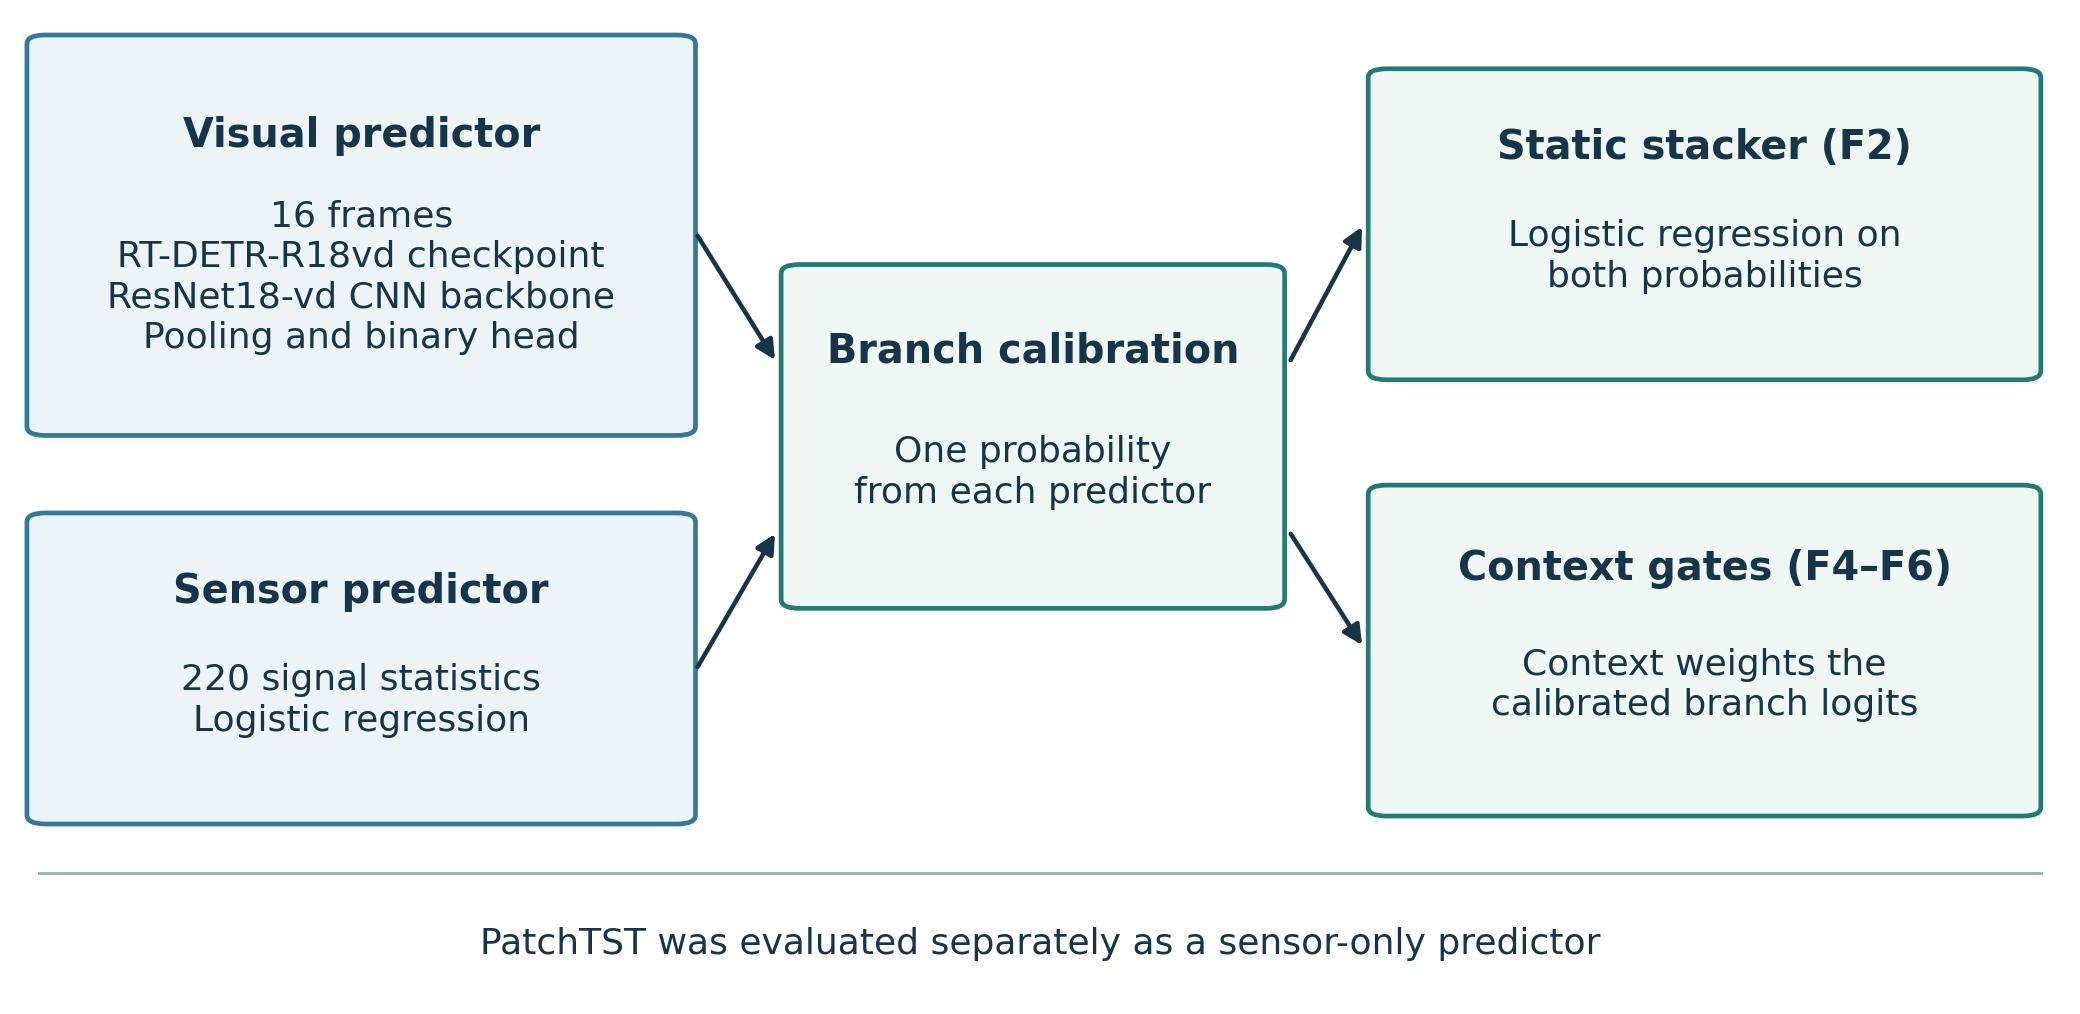
\includegraphics[width=\textwidth]{figures/fusion_interfaces.png}
\displaynote{The stacker and all three gates used the statistical sensor predictor. PatchTST was evaluated separately as a sensor-only comparator in the core experiment. Each branch supplied a calibrated probability. The gates converted those probabilities to logits before weighting them.}
\end{figure}
\section{Component Selection Criteria and Implementation Mapping}
Selection considers target relevance, observation horizon, group support, training exposure, incremental input value, calibration, and computational scope. A frozen representation is attractive when nested fits must remain feasible; a statistical reference is essential when a larger encoder may overfit or be insufficiently trained. An adaptive fusion stage is warranted for investigation when reliability varies and meaningful quality signals exist, but it must still beat an exposure-matched simpler control.

The original visual, audio and sensor question consequently includes implemented and candidate components. AST supplies a pretrained spectrogram-Transformer option, with reported scores distinguishing checkpoint weight averaging from multi-model ensembles and showing task-dependent transfer benefits \citep{P011}. Alignment checks prevented admission of a predictive audio branch here. The published ViT, Video Swin, AST and MOMENT evaluations provide architectural precedents. The executed comparison instead concerns frozen CNN features, statistical sensors, a scratch temporal encoder and explicitly defined fusion interfaces.

The implementation map (Appendix~\ref{app:reproducibility}, \EvidenceRef{E110}{}) records executed paths; Appendix~C lists configuration details. Each performance estimate applies to the combination of components, cohort and metric evaluated in that experiment. The studies did not jointly test all components that performed well individually.

\chapter{Research Design and Shared Methodology}
\label{ch:methodology}

\section{Relationship Between the Research Questions and Case Studies}
The five studies address the representation and fusion questions (SQ1 and SQ2) by comparing predictors on the same target and assessment units within each study. For robustness (SQ3), REASSEMBLE and MSM compare learned fusion under controlled input degradation. HANDOVER evaluates degradation and known input loss for the simpler baselines. PHM leaves the robustness of visual--sensor fusion open, and the ViFailback analysis includes no completed stress results for the reported fusion models. For SQ4, the evidence includes target validity in regression, probability quality and threshold outcomes in classification, and estimates of uncertainty or computational cost where available.

The five implemented studies carry the original welding question into tasks with different prediction targets. In PHM, photographs define the gear-condition proxy that sensor models predict. REASSEMBLE provides the principal comparison on completed robotic actions. MSM tests the procedure on abnormal milling intervals. ViFailback tests complete manipulation episodes across held-out tasks and separately examines transfer of a visual encoder. In HANDOVER, video and force--torque signals cover a common observation window for each labelled trial. The official test split supports evaluation of single-input predictors and fixed averaging. Fitting the proposed learned fusion model would also require participant identifiers for constructing training predictions (Appendix~\ref{app:handover}).

Figure~\ref{fig:research-workflow} shows how the welding objective relates to the five experiments. Each comparison required a defined target, paired observations and an assessment group appropriate to that target.
\begin{figure}[htbp]
\caption{Workflow for Data Qualification and Model Evaluation}\label{fig:research-workflow}
\centering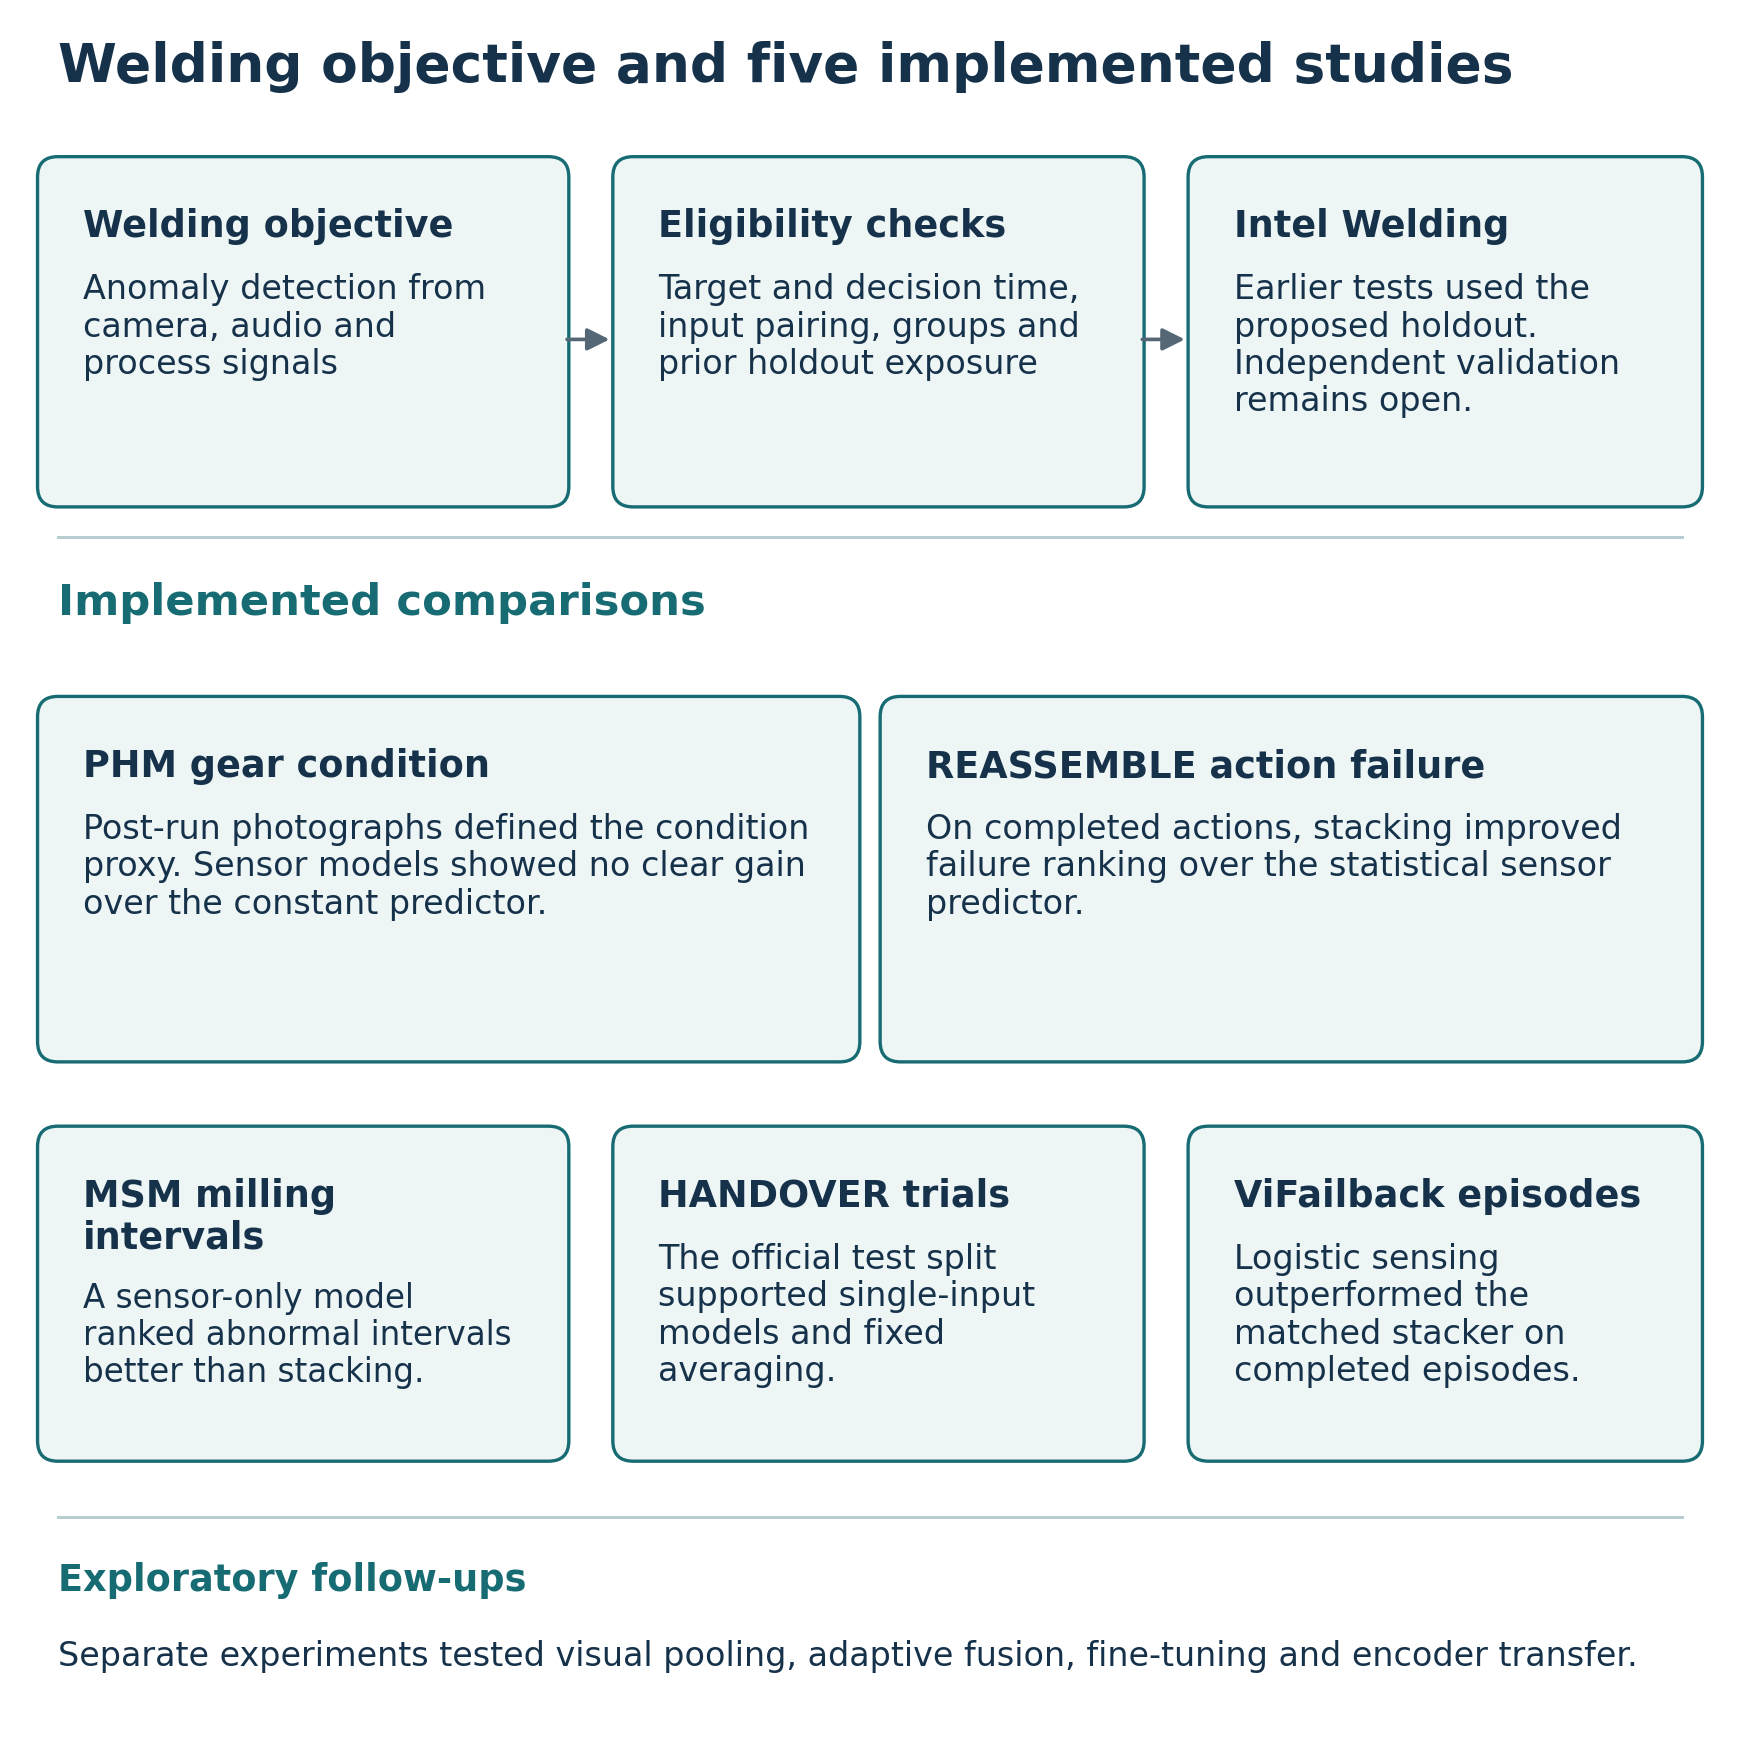
\includegraphics[width=\textwidth]{figures/research_workflow.png}
\displaynote{The five studies used different prediction targets. Each finding refers to the comparison within that study.}
\end{figure}

\section{Dataset Selection Criteria and Research Chronology}
Selection considered access, relevant physical observations, interpretable targets, correspondence, group identifiers, class support, and computational feasibility. These criteria changed what could be evaluated. A public multimodal dataset may lack a usable target for the proposed task; another may have labels but too few independent groups for the desired evaluation.

The initial welding proposal preceded the PHM and REASSEMBLE studies. Later investigations addressed uncertainties exposed by those studies: stronger sensor references, visual pooling, fine-tuning budgets, quality-conditioned fusion, and external adaptation. The October alignment record retained the original four-question hierarchy after a narrower quality-gate investigation had been considered. Follow-ups motivated by observed outcomes were exploratory. Appendix~G summarizes the scientific chronology.

The experimental inventory identifies the completed comparisons and their source records. For ViFailback these cover the original frozen study and the matched frozen and donor-backbone comparisons. The computational budget at thesis freeze placed target-CNN fine-tuning and the SQ3 corruption evaluation outside the final scope. The source manifest identifies the inspected Git commit \texttt{e32ec43aef69cc58adff0ea91e508308041598c5} and records hashes for selected files, including uncommitted report outputs.\ev{Remote source manifest}{\EvidenceRef{E111}{}, \EvidenceRef{E109}{}}

\section{Intel Welding Feasibility Assessment and Resulting Scope Decisions}
The Intel foundation scripts inspect sample structure, readability, timing/session fields, and duplicates. Their configuration disables a final test, and the audit encodes that earlier context evaluation had exposed the proposed holdout population. Reusing that population would preclude an independent confirmatory test. The retained subset does not establish the full original label mapping or a completed native multimodal classifier. Earlier contextual baseline reports therefore provide historical feasibility information, rather than evidence that a proposed Transformer-fusion architecture failed empirically.\ev{Intel Welding feasibility assessment}{\EvidenceRef{E019}{inspect\_sample, audit\_split, main}, \EvidenceRef{E018}{}, \EvidenceRef{E003}{section 3.1}}

The project record attributes the shift to PHM and REASSEMBLE to an agreement with the supervisor reported by the researcher. The two studies address the original architectural and evaluation questions using different tasks, modalities, and targets. No claim of welding deployment or welding-domain validation follows from success in robotic assembly or milling.

\section{Dataset Admission and Preparation Checks}
Admission requires an explicit sample manifest. Each row should identify its prediction unit, target source, physical group, input paths, interval boundaries, availability, and any exclusion reason. Visual checks cover decoding, frame support, geometry, and the distinction between visible context and visible target evidence. Sensor checks cover channel ordering, units, timestamps, gaps, duplicated rows, missing values, and the meaning of interpolation or aggregation. Pairing checks ask whether the two inputs describe the same event, not merely whether both files exist.

An exclusion is consequential when it changes the target distribution or removes difficult failures. Counts before and after exclusion are therefore part of the evaluation. Quarantined samples retain their original labels. In MSM, timing-alias correction and grouping support determine admission; in ViFailback, duplicate or invalid telemetry and video failures affect the cohort. Technical quality control cannot independently validate semantic labels, physical damage, or a camera's visibility of the relevant phenomenon.

\section{Target Provenance, Prediction Units, and Available Inputs}
A task record states what is being predicted, how the reference is obtained, and which inputs would be available at the prediction time. PHM's image-derived candidate-area score is a provisional condition proxy. Sensor prediction of that score measures agreement with the construction, not verified wear or remaining useful life. REASSEMBLE labels complete action outcomes. ViFailback labels complete episodes. MSM uses a declared mapping of milling labels, with alternatives treated as sensitivity analyses. The physical interpretation of a score depends on these definitions.

The observation horizon is explicit. Sampling frames from the entire action allows retrospective recognition of its outcome; it does not demonstrate warning before that outcome. Likewise, controller aggregates can summarize an interval only after it has elapsed. A prospective experiment would need a fixed decision time, causal preprocessing, a definition of lead time, and labels aligned to that horizon. The offline classifications do not measure lead time.

Process identity, duration, time index, or extraction latency can become predictive shortcuts. The PHM visual head receives extraction latency alongside its image features. A process-context gate may exploit action-specific prevalence, so its improvement would not automatically show that it recognized physical sensor reliability. Relevant context-only and constant-adjustment controls test narrower alternatives where available.

\section{Grouping, Data Splits, and Leakage Prevention}
The split unit determines the scope of the generalization claim. The principal PHM sensor protocol holds out gear experiments, REASSEMBLE groups actions by recording, MSM examines experiment and date groupings, and ViFailback separates tasks. HANDOVER retains the published trial partitions. The available identifiers allow neither independent verification of the reported participant separation nor construction of participant-disjoint inner folds. For MSM, a date can span multiple tools or operators, and physical equipment may recur across dates. A claim about a new machine or factory requires grouping information at that level.

Within an outer split, feature scaling, imputations estimated from data, model selection, calibration, thresholds, and fusion fitting must use training-side information. For stacking, the training bank contains predictions from models that did not fit the corresponding labels. If a branch recipe is selected, that selection also belongs inside the permitted training hierarchy. Even with an out-of-fold prediction head, assessment information can enter the model through an encoder or normalizer fitted on the full dataset. Each base prediction for the original REASSEMBLE stacker came from a branch fitted without data from the corresponding recording. Within each outer split, internal stacker validation reused the same out-of-fold (OOF) prediction bank built from the outer training recordings. A branch that supplied a prediction for a stacker training row could have been fitted on recordings held out for that stacker validation split. The outer-assessment recordings remained excluded from fitting. Full independence at the deeper validation stage has yet to be demonstrated. This dependency limits the claim of strict nesting.\ev{Original stacker-validation dependency}{\EvidenceRef{E004}{section 15.4}}

The original REASSEMBLE cohort comprises 4,530 actions, 509 failures, and 148 recordings. Its five held-out partitions together cover this population. A later 753-action comparison uses one of these exposed outer partitions, not a new external holdout. Cohort reconciliation uses sample and recording identities to distinguish overlapping and identical populations. An earlier summary listed 28 recordings. The sample identifiers establish that this subset contains 26.\ev{Assessment sample and recording identifiers}{\EvidenceRef{E052}{}}

A specific PHM four-arm runner fits a normalizer before a loop that changes the held-out experiment. Its held-out experiments therefore contribute to preprocessing. The principal PHM runner fits its normalizer inside each fold. A fold-isolated estimate for the four-arm comparison would require repeating that experiment.

\section{Model Fitting, Selection, Calibration, and Threshold Procedures}
Each comparison defines trainable components, initialization, selection candidates, training budget, and stopping rules. An epoch count alone does not establish matched optimization if samples, batch sizes, early stopping, or cached representations differ. The experimental programme included original comparisons, exploratory pilots and matched short-budget diagnostics. Some larger experiments completed only a subset of the planned fits.

Calibration maps raw model scores to probabilities using training-side predictions. Discrimination and calibration are different properties: a monotonic score transformation can preserve ranking while changing probability errors. The core branch calibrators use sigmoid logistic maps on selected inner out-of-fold scores. The original softmax gates have no free final intercept or post-gate calibrator, whereas F2 has a free intercept and no additional post-stacker calibration. These function-class and post-processing choices remain visible in the comparison \citep{Guo2017Calibration}.

A decision threshold is selected using permitted training predictions and a stated objective, such as balanced accuracy. The original implementation searches a grid from .01 to .99. Such a threshold is a protocol choice, not a cost-optimized industrial alarm policy. At that threshold, sensitivity, specificity, precision, and false-alert burden give a clearer account of performance than accuracy alone. Assessing operational acceptance also requires information about stakeholder costs.

\section{Metrics and Uncertainty Estimation}
For regression, MAE is $n^{-1}\sum_i|y_i-\hat y_i|$ and RMSE is $\sqrt{n^{-1}\sum_i(y_i-\hat y_i)^2}$. Both inherit the units and validity of the target. $R^2$ compares squared error with a reference denominator and can be unstable or negative in small held-out groups. Tooth-level and run-level PHM metrics remain separate because their targets and dependence differ.

For classification, the main ranking statistic is average precision as implemented by \texttt{average\_precision\_score}. With recall increments $\Delta R_k$ and precision $P_k$, $\mathrm{AP}=\sum_k\Delta R_kP_k$. It is not the same numerical quantity as trapezoidal area under a precision--recall curve. AUROC measures ranking over negative--positive pairs; AP depends strongly on the positive-class prevalence. Precision--recall analysis is particularly useful for imbalanced outcomes, but scores from different prevalences should not be treated as a model ranking across datasets \citep{Saito2015PrecisionRecall}.

Binary failure AP, success AP, their macro average, mean-fold AP, and AP computed from pooled held-out predictions are different estimands. The nonlinear metric implies that mean-fold AP generally differs from pooled AP. ViFailback tables name macro AP explicitly; REASSEMBLE's original headline uses pooled failure AP. Threshold metrics and Brier score $n^{-1}\sum_i(p_i-y_i)^2$ address different questions. Interpret calibration summaries in light of how the bins were defined and how many observations contributed.

For a paired model comparison, define $\Delta=\mathrm{AP}(p_A,y)-\mathrm{AP}(p_B,y)$ on identical rows. A cluster bootstrap samples dependence groups with replacement and recomputes the paired difference. Core REASSEMBLE reports use 2,000 recording-level replicates; a PHM report uses 10,000 run-cluster replicates over 20 runs. These are intervals conditional on the saved fitted models and the chosen resampling unit. They do not capture all retraining, model-selection, seed, or new-site uncertainty. Five MSM dates provide a particularly small basis for a date-cluster interval. Cross-validation folds are overlapping training experiments, not independent replications; uncertainty should not be inferred from a naive standard error over folds \citep{Bengio2004CVVariance}.

\section{Robustness Evaluation Design}
A robustness test specifies how the failure occurs, which modality and stage it affects, and how severe it is. It also reports the number of realizations, any exposure to the failure during training, and the observations and metric used. The availability mask identifies a stream declared missing. A corrupted stream can remain available and supply a prediction. Corrupting pixels targets a different stage from corrupting cached visual features. Sensor corruption can affect raw channels, statistics, or logits. Recompute any quality features meant to describe the corrupted observation.

Clean and degraded absolute scores are both needed. A smaller clean-relative drop can coexist with worse absolute performance. A gate can shift weight away from a corrupted modality while still underperforming the intact unimodal predictor. The relevant controls include the surviving branch, a static fusion model with matched augmentation exposure, and any simpler parameterization needed to isolate adaptation. Training with modality dropout establishes exposure to missing inputs. Recovery is measured on held-out cases where the input is absent.

The original two-input gate routes a single surviving branch with weight one. With fixed branch outputs this makes single-input predictions identical regardless of gate training. Both missing inputs raise an error; no predictive result is attributed to that state. These tests leave open the effects of clock offsets, previously unseen machines and novel failure mechanisms.

\section{Reproducibility and Experiment Provenance}
The core REASSEMBLE visual branch loaded the pretrained RT-DETR-R18vd checkpoint through Hugging Face Transformers and selected its ResNet18-vd convolutional backbone. The backbone stayed frozen while a separate binary classifier learned from its pooled features. The same library supplied the PatchTST sensor encoder, initialized from scratch \citep{Wolf2020Transformers}. PyTorch trained the neural prediction heads with AdamW \citep{Paszke2019PyTorch}. Scikit-learn supplied the grouped stratified splits and logistic regression baseline \citep{Pedregosa2011ScikitLearn}. The PHM image regressor used the Ultralytics RT-DETR-L prediction path to extract intermediate feature maps \citep{UltralyticsRTDETR}.\ev{Library use in executed models}{\EvidenceRef{E064}{}, \EvidenceRef{E065}{}, \EvidenceRef{E067}{}, \EvidenceRef{E046}{}, \EvidenceRef{E033}{}, \EvidenceRef{E004}{P01}}

Verification used archived source code, configurations and results. Where saved predictions were available for selected comparisons, metrics could also be recalculated. These checks used the existing fitted models' outputs without retraining or rerunning inference on raw observations. For historical runs, the recorded configuration and results identify which code path produced the reported comparison.

The evidence files record source paths and hashes for the inspected implementation, the assessment cohorts and the metric definitions. Literature extraction records connect bibliographic metadata and relevant passages to individual publications.

\section{Computational Constraints and Exploratory Versus Confirmatory Analysis}
Resource limits motivated cached features, compact heads, small selection grids, and bounded follow-ups. Those choices define the tested system. They cannot justify declaring an undertrained architecture intrinsically unsuitable or an unfinished arm inferior. Timings must state whether they measure warm extraction, a head fit, or an end-to-end pipeline, with device and preprocessing included where available.

The work is primarily exploratory and retrospective. Repeated exposure to the same assessment cohort, follow-ups selected after inspecting results, and later protocol adjustments limit confirmatory interpretation. A future confirmatory study should freeze targets, cohort construction, selection rules, primary contrasts, corruption operators, and claim criteria before the assessment is opened. The conclusions are conditional on this exploratory development history and on the saved evidence available for each study.

\chapter{PHM Case Study: Target Construction and Condition Prediction}
Across twenty gear runs in three held-out experiments, combining three groups of sensor features gave a mean absolute error of 0.8238 percentage points against a photographic condition proxy. A predictor that returned the training mean gave an error of 0.8042. Both errors measure agreement with an image-processing rule applied to post-run tooth photographs. The records contain no independent measurement of the damaged area against which to validate that rule.

In retrospect, PHM serves as a methodological negative control for the wider fusion comparison. Even a reduction in prediction error would need independent validation before it could be interpreted as better damage measurement. The study therefore distinguishes changes in the target from changes in the predictor. Image-only and supplementary experiments had different targets or assessment populations. Under the official challenge protocol, periodic photographs were available during training, whereas deployment relied on sensor measurements \citep{PHM2026Challenge}.

\begin{figure}[htbp]
\caption{PHM Scalar Regression From Post-Run Photographs}\label{fig:phm-route}
\centering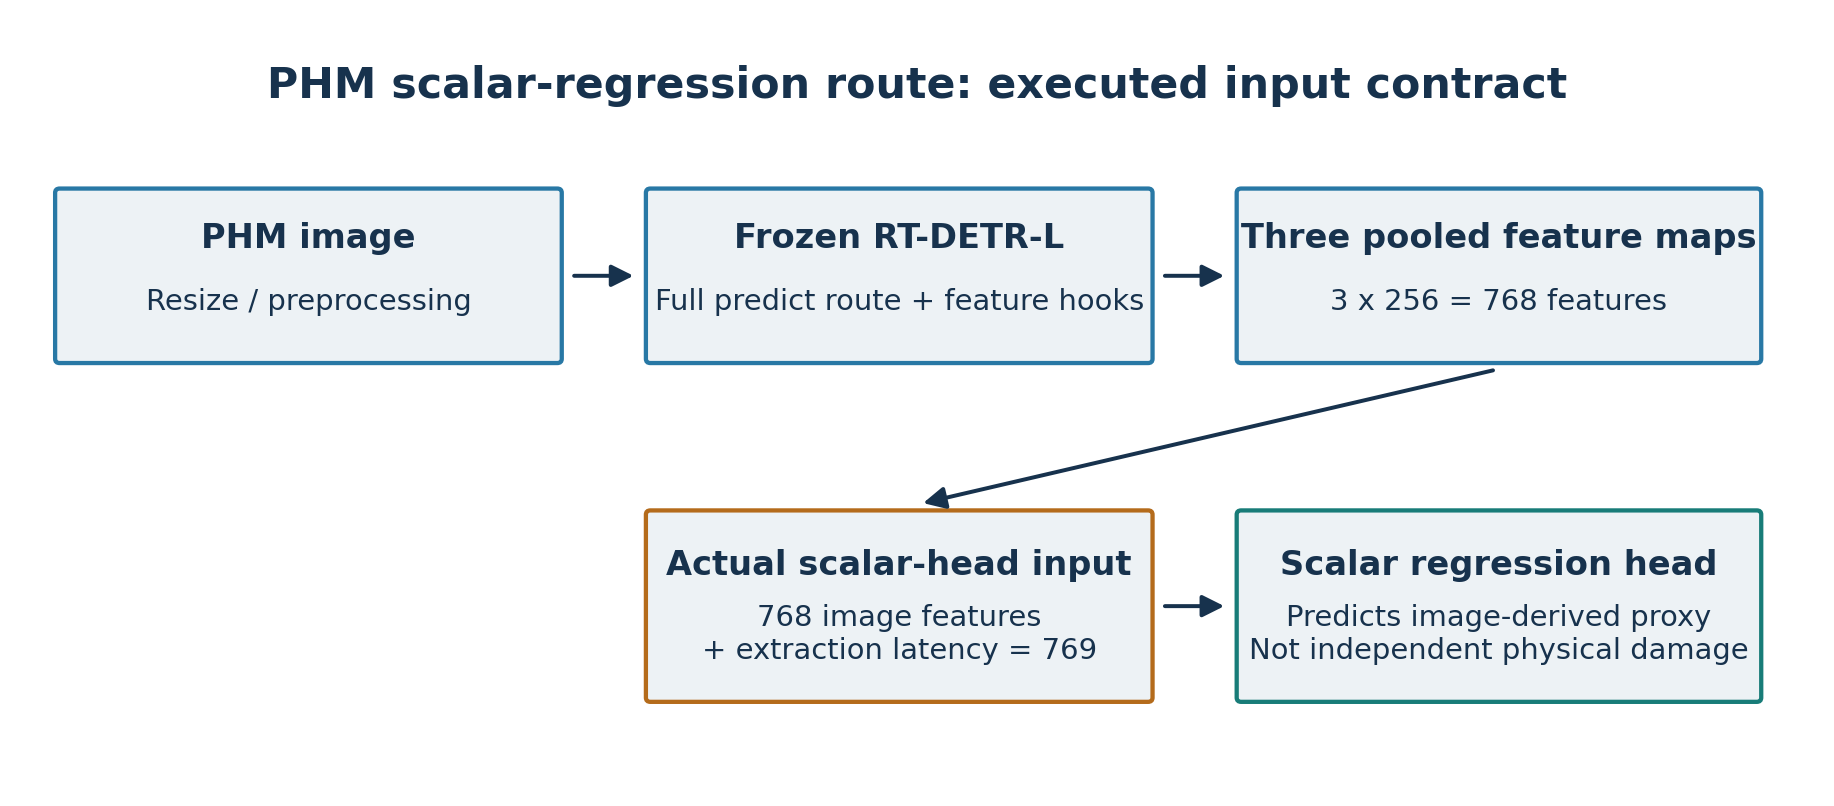
\includegraphics[width=\textwidth]{figures/phm_executed_route.png}
\displaynote{The extraction code adds latency to the 768 image features, producing a 769-dimensional input to regression.}
\end{figure}
\section{Study Objective and Relationship to the Research Questions}
For SQ1, the image and sensor experiments assessed whether frozen visual features and temporal sensor representations could reproduce a specified target. For SQ2, the principal fusion comparison combined context, root-mean-square (RMS) vibration and condition indicators, all available at inference. It did not test joint image--sensor inference. For SQ3, a predictor that already returns nearly constant values can appear insensitive to corruption, so its clean-input error matters. For SQ4, the training-mean comparison asks whether measured sensor inputs improved prediction over a rule that ignores them at inference. It cannot establish whether the photographic target measures damage. That question requires a physical reference independent of the rule.\ev{PHM target and deployment inputs}{\EvidenceRef{E021}{}}

\section{Dataset Overview and Acquisition Structure}
The retained population contains EXP-A runs 1--5, EXP-B runs 1--7 and EXP-F runs 1--8: twenty nominal run units across three experiments. A run can contain multiple tooth photographs, camera-sequence views, high-frequency vibration members, low-frequency context measurements and condition-indicator records. An image, a minute-level feature row and a run are consequently different observational units. Repeated views and long sensor sequences increase the number of stored observations without increasing the number of independently acquired experiments to the same extent.

Experiment and run identifiers are retained through derived manifests. Tooth identity and image role define target generation, whereas archive/member identity and measurement provenance define sensor features. Their correspondence is principally at run level. This supports joining measurements to a post-run proxy, rather than asserting hardware-synchronized image/sensor events or prospective image availability. Evidence covers these manifests and inspected implementation, with incomplete independent reinspection of raw archive contents.\ev{PHM experiments and acquisition sources}{\EvidenceRef{E020}{}}

\section{Dataset Challenges and Supervision Limitations}
The target depends on acquisition geometry, illumination, texture and image-processing choices as well as possible surface damage. In EXP-A and EXP-B, tooth indices 1--4 and 5--28 had different image-role coverage. Because tooth identity and view role were confounded, comparing their candidate-area percentages could mix material differences with acquisition differences. The v3 exclusion described below addresses this particular problem; it does not independently validate the retained twenty-four teeth.

The organizers reported possible overlap for EXP-A Run-2. A separate analysis addressed equality between derived sequences. A tutorial reports equality of 372 feature rows across 72 derived spectral features for two runs. That is evidence about its extracted representation, not byte-level proof that complete raw archives are identical. Both nominal runs remain visible in the historical analysis. The small number of independent experiments, unequal run lengths and changing acquisition conditions limit broad generalization even when train/test identifiers do not overlap.\ev{Organizer-reported overlap in EXP-A}{\EvidenceRef{E020}{}}\ev{Derived spectral diagnostic}{\EvidenceRef{E037}{}}

\section{Preparation, Exploratory Analysis, and Pre-Checks}
Preparation distinguished structural eligibility from scientific validity. Source manifests retained experiment, run, tooth and image identities; sensor inspection considered channel presence, units, finite values, temporal coverage and operating-state eligibility. The early EXP-A exploration used runs 1, 3 and 5 and remains a deliberately narrower historical analysis, not evidence that every later included run received the same exploratory scrutiny. Its protected outputs were not rewritten to match the later all-run population.

Minute-level representations summarize process and sensor variables instead of passing the entire waveform to the principal model. Timestamp and coverage checks support sequence assembly, while aggregation can discard transients. The high-frequency tutorial has different representation provenance. Duplicate diagnostics, missingness masks and exclusions therefore remain tied to their producing configurations; combining them would define a different dataset from that which generated the historical predictions.\ev{PHM domain implementation}{\EvidenceRef{E034}{}}

\section{Task Formulation and Target-Version History}
The current-end-of-run target is a percentage of a fixed visible-flank region classified as candidate area. It is not remaining useful life, a native failure class, or a calibrated physical spall-area measurement. A run-level target aggregates the largest three tooth values. Raw target values and a causal monotonic transformation are separate outcomes; monotonic processing cannot serve as independent evidence that the raw measurements track deterioration.

\begin{table}[htbp]
\caption{Versions of the PHM Condition Proxy}\label{tab:phm-target-lineage}
\centering\small
\begin{tabularx}{\textwidth}{@{}P{18mm}YP{18mm}P{23mm}Y@{}}\toprule
Version & View rule & Teeth/run & Materialized rows & Interpretation\\\midrule
v1 & maximum candidate ratio & 1--28 & 560 & superseded ROI/threshold\\
v2 & maximum candidate ratio & 1--28 & 560 & retained historical artifact\\
median--28 & median rule in code & 1--28 & none & referenced, not materialized\\
v3 & one deterministic view & 5--28 & 480 & current retained target\\\bottomrule
\end{tabularx}
\displaynote{Each row count refers to tooth--run combinations. The run-level target aggregates the three highest tooth values where defined.}
\end{table}

Version changes alter the quantity being predicted. Changing ROI geometry and a residual threshold between v1 and v2 altered the proxy scale by approximately a factor of six according to the target-version records. A median-view code state retained the v2 label without a corresponding production artifact. Under v3, a canonical tooth view is selected where available, otherwise the earliest camera-sequence view by embedded time. Identical numerical constants in two versions can arise from unchanged top-three teeth and do not prove identical measurement rules.\ev{Versions of the photographic condition proxy}{\EvidenceRef{E023}{}}

\section{Investigation A: Image-Derived Target Construction and Assessment}
The visual investigation has three distinct layers: producing a deterministic target, fitting a model to that target, and assessing how closely that target represents physical damage. The first two layers can be inspected from code, saved targets and prediction artifacts. The third requires external reference evidence. Agreement with a heuristic mask is insufficient because it evaluates reproduction of the same rule that supplied supervision. This distinction also applies to the detector trained on heuristic pseudo-boxes: its localization metrics are defined relative to those boxes, not expert-annotated defects. The separate scalar, detector and multitask routes therefore remain different experiments with different outputs and comparison units.\ev{Visual prediction experiments}{\EvidenceRef{E025}{}}

\subsection{Motivation and Target Definition}
Without organizer-supplied continuous damage labels, an explicit and reproducible candidate-area statistic offered an engineering starting point. The implementation measures dark, horizontally extended regions within a chosen flank ROI. Its percentage denominator is the ROI area, so a change in ROI changes the numerical scale even if the same pixels are selected. The term ``candidate'' is substantive: reflectance, machining texture and acquisition artifacts may satisfy the image rule without being physical damage. The target can consequently support a study of proxy prediction and measurement sensitivity. It cannot by itself support a claim about tooth material loss or maintenance necessity.\ev{Candidate measurement function}{\EvidenceRef{E035}{measure\_damage\_candidate}}

\subsection{Image Processing and Aggregation}
The inspected target code converts RGB to Lab luminance, applies CLAHE, estimates a smooth background, and obtains a dark residual. Robust standardized residuals define candidate pixels; morphological opening and closing and component-size/aspect criteria retain extended regions. Candidate pixels divided by ROI pixels give the per-view percentage. Historical v2 view maxima and the v3 deterministic-view rule then produce tooth values, followed by the top-three run mean.

The PHM scalar baseline invoked the Ultralytics RT-DETR-L prediction path and recorded intermediate maps from three layers. The regression head used 768 spatially pooled image features and one additional value, extraction latency. Latency depends on the computing environment and can confound interpretation of the image-regression result. Separate PHM detection and multitask experiments used heuristic pseudo-box supervision. The core REASSEMBLE classifier used the ResNet18-vd CNN backbone inside its RT-DETR-R18vd checkpoint (Chapter~6).\ev{Extraction implementation}{\EvidenceRef{E033}{extract\_features}}\ev{Image features and latency covariate}{\EvidenceRef{E024}{}}

\subsection{Assessment Procedure and Available Reference Evidence}
Prediction error measures how well a model reproduces the target on held-out images, teeth or runs under the specified split. The separate appearance assessment compares selected images with human judgments. A continuous physical-area reference would require independent measurements or area annotations. The retained appearance-based and AnomalyDINO-style diagnostics are useful for finding conspicuous disagreements, but their selection and development exposure prevent treating them as an untouched validation cohort.

The retained evidence contains no independent expert area masks or physical reference measurements that establish population-wide target accuracy, calibrated area percentages or a defensible damage/no-damage operating threshold. A prediction cannot independently resolve ambiguity in the appearance used to construct its training label. These limits constrain subsequent interpretation even if a target-emulation score appears favorable.\ev{Photographic proxy and appearance diagnostics}{\EvidenceRef{E022}{}}

\subsection{Target Scaling and Validation Limits}
The two reported baseline errors refer to different versions of the photographic target. Under the fixed EXP-B-to-EXP-F comparison, the training-mean run MAE is 0.6797 percentage points for v2 and 0.7348 for v3. The difference follows target construction, not scalar-versus-profile aggregation: the top-three mean of the mean sorted training profile equals the corresponding scalar training mean by linearity.

Detector diagnostics report very small attainable recall against dense heuristic boxes and a mismatch between predicted-box and pseudo-box scales. Those observations qualify this training recipe and supervision geometry. Activation energy near an apparent surface region does not independently prove correct localization or identify a unique causal failure mechanism. Likewise, the saved image-regression row included in a later summary is explicitly not LOEO and lacks EXP-B predictions. Its assessment population therefore differs from that of the twenty-run sensor LOEO comparison. The retained visual work establishes reproducible implementation and consequential supervision limitations, rather than verified physical damage detection.\ev{Training-mean errors by target version}{\EvidenceRef{E023}{}}\ev{Detector diagnostics}{\EvidenceRef{E036}{}}

\section{Investigation B: Sensor-Based Condition Prediction}
The sensor investigation asks whether run-level inputs available without post-run imaging predict the provisional condition statistic. Images supply supervision in this task, not a deployable inference branch. The comparison includes a training-mean constant, a single sensor encoder and combinations of sensor-feature groups. Maintaining that distinction prevents the broad phrase ``multimodal fusion'' from obscuring a change in experimental question. A successful result would establish prediction of a particular proxy under a particular split. A failed result leaves several possible explanations, including target noise, acquisition shift, limited independent training support, representation loss and optimization limits. The observed comparison alone does not identify which explanation dominates.\ev{Sensor and fusion implementation}{\EvidenceRef{E032}{}}

\subsection{Inputs and Preprocessing}
The retained minute-feature configuration names nine base variables: speed, torque, temperature, axial RMS, radial RMS, FM4, NA4, M6A and ALR. Seven summaries per base variable---mean, standard deviation, median, minimum, maximum, last value and slope---plus missingness indicators yield 72 channels. These are variable-length sequences of engineered features. They are not 72 raw accelerometer channels or a raw-waveform Transformer input. A separate spectral analysis constructs a 72-feature array from high-frequency vibration.

The custom PHM model forms shared channel-wise patches and applies positional encoding, a Transformer encoder and masked pooling. Padding and any-valid-time patch masks are explicit in source. Their existence does not prove historical invariance to batch length or resolve earlier patch-grid concerns. Train-only transformations are supported for the principal LOEO runner; an audit-reported normalizer fitted before a different four-arm loop is a separate limitation.\ev{Minute-feature configuration}{\EvidenceRef{E027}{}}\ev{Patch and mask computation}{\EvidenceRef{E031}{patchify}}

\subsection{Reference Predictors and Model Configurations}
The training-mean constant is essential because the target scale and between-experiment distribution can make a visually plausible prediction uncompetitive. Ridge regression supplies a regularized non-temporal reference, with the retained configuration searching alpha values 0.01, 0.1, 1, 10 and 100. The custom PatchTST scalar path uses width 32, two encoder layers, four heads, feed-forward width 64, patch length 16 and stride 8 in the inspected configuration. An optional profile head constrains outputs to sorted ascending tooth statistics through positive increments; it does not preserve positional tooth identity.

The retained \texttt{fused\_all\_three} gives context, RMS and condition-indicator groups separate encoders, concatenates their embeddings and applies a scalar head. This is feature-level multi-source sensor fusion despite the class name \texttt{LateFusionRegressor}; neither probability stacking nor visual--sensor inference describes this path. The later four-arm code additionally distinguishes two RMS sources and an empty encoder group, which is excluded. Its process-conditioned fusion derives allocation from context features. These comparisons do not supply the unavailable inference-time tooth image. Configured epoch caps remain separate from actual fold histories.\ev{Regression and Ridge implementation}{\EvidenceRef{E032}{}}\ev{Inputs to PHM feature fusion}{\EvidenceRef{E004}{section 12.4}}\ev{Group provenance and gate}{\EvidenceRef{E030}{}}

\subsection{Training and Evaluation Protocol}
The historical fixed split trains on EXP-B, validates on EXP-A and assesses EXP-F. It contains seven training, five validation and eight test runs. The principal retained LOEO procedure instead rotates the assessment experiment while keeping a separate remaining experiment for validation: train F/validate B/test A; train F/validate A/test B; train B/validate A/test F. Thus ``leave one experiment out'' does not mean fitting on both remaining experiments. Only three experiment identities support this analysis.

The retained runner refits its normalizer on each training experiment. This is a materially stronger isolation claim than can be made for the distinct four-arm diagnostic whose preprocessing was fitted outside its changing fold loop. The analysis identified the target version from the selection settings, target hashes and source arrays because some configuration labels referred to an earlier version. Missing historical fold records limit retrospective verification.\ev{Principal LOEO runner}{\EvidenceRef{E028}{}}\ev{Target provenance}{\EvidenceRef{E023}{}}

\subsection{Results and Uncertainty}
Table~\ref{tab:phm-loeo} reports the retained twenty-run summary on the provisional target scale. Lower MAE and RMSE are preferable; rank correlation addresses ordering rather than calibration. The constant's nonzero pooled rank statistic reflects changing fold-specific constants, not informative within-fold ranking.

\begin{table}[htbp]
\caption{PHM Prediction Error Across Held-Out Experiments}\label{tab:phm-loeo}
\centering\small
\begin{tabular}{lrrrr}\toprule
Model & MAE & 95\% interval & RMSE & Spearman\\\midrule
Training-mean constant &0.8042 &[0.5769,1.0360]&0.9608&-0.0354\\
Single encoder &0.9415 &[0.6754,1.2264]&1.1337&-0.2053\\
Three-group fusion &0.8238 &[0.5527,1.1015]&1.0332&-0.1046\\\bottomrule
\end{tabular}
\displaynote{The analysis includes 20 nominal run units. Errors are expressed in percentage points of provisional candidate area. Run-cluster bootstrap intervals are conditional on the fitted models.}
\end{table}

The observed difference in mean absolute error between three-group fusion and the training mean was $+0.0196$ percentage points across the twenty runs. The mean of the paired run-bootstrap differences was $+0.0177$ percentage points, with a 95\% interval of $[-0.1962,0.2278]$. The interval allows lower error for either predictor. The study used no prespecified equivalence margin.\ev{Observed errors and paired bootstrap}{\EvidenceRef{E026}{}, \EvidenceRef{E004}{section 12.5}}

\subsection{Interpretation and Limitations}
The retained learned predictors do not establish an improvement over the constant under this task and protocol. That conclusion is narrower than ``the sensors have no damage information.'' The target may not align with the physical signal, a model can be underfit or overfit, and cross-experiment acquisition differences may dominate the small training population. Twenty nominal runs also do not eliminate dependence caused by repeated or equal derived sequences.

Run-cluster intervals describe resampling of saved outcomes conditional on fitted models. They do not quantify full training-seed variation or uncertainty over a population of independent test machines. With only three experiments, the number of genuinely different deployment domains remains small. The unresolved target meaning, the profile's loss of tooth identity and padding/provenance concerns additionally limit interpretation. These qualifications do not erase a negative comparison; they identify which hypothesis it actually challenges.\ev{PHM comparison and target validity}{\EvidenceRef{E106}{}}

\section{Additional Diagnostic Experiments and Evaluation Sensitivity}
Supplementary analyses investigate why the original routes were insufficient, without replacing the principal comparison. The HF/spectral tutorial reports MAE 1.2203 for its full 72-feature model against a v2 constant MAE 0.6797 on eight EXP-F runs. Reduced-feature variants performed better than that full model but none beat its constant. Repeatedly inspecting feature subsets on the same test split makes this a development diagnostic, not independent confirmation of the selected subset. Its strong causal language about overfitting or complete archive duplication exceeds what feature tables alone establish and is not adopted here.

The four-arm study compares group regressors, concatenation, affine late fusion and context-conditioned embeddings, but its preprocessing-isolation concern prevents merging its results with principal LOEO. Raw-vibration and tooth-sector screens, AnomalyDINO sweeps, odd/even views, synthetic controls, teacher/oracle constructions and monotonic rescoring address separate uncertainties. An oracle or target-derived synthetic feature can demonstrate pipeline capacity without demonstrating deployable information. Detailed diagnostic tables belong in Appendix D with their own target and exposure labels.\ev{HF diagnostic report}{\EvidenceRef{E037}{}}\ev{Four-arm implementation}{\EvidenceRef{E029}{}}

\section{What the PHM Study Establishes and Leaves Unresolved}
Neither the single sensor encoder nor the three-group model improved on the training mean in the observed run-level comparison. The paired interval for three-group fusion included both lower and higher error. Changing the photographic target also changed the constant predictor's error on a fixed split. The comparison therefore challenges the inference that adding sensor representations improves prediction of this proxy across experiments.

Optimizing a predictor for physical damage would first require checking the proxy against independent damage measurements or expert area annotations. Until then, the error estimates quantify agreement with the photographic rule. The study also leaves advance warning, remaining useful life and response to natural sensor failure unresolved. Differences in targets, prediction units and preprocessing, including the four-arm experiment's shared normalizer, prevent a direct comparison across all PHM fusion models.\ev{Photographic target versions}{\EvidenceRef{E023}{}}\ev{PHM experiment configurations}{\EvidenceRef{E025}{}}

\section{Implications for Subsequent Dataset and Architecture Choices}
PHM was undertaken within the architecture programme motivated by robotic welding, rather than as a prespecified feasibility stage designed around its eventual negative result. The subsequent move to REASSEMBLE responded to supervision and comparison limits: recorded action outcomes, visual and sensor inputs at a common completed-action horizon, and more recording groups. The empirical task changed from a photograph-derived gear-condition proxy to retrospective manipulation failure, retaining the questions about representation, fusion and robustness. This progression does not validate a welding classifier or establish that visual and vibration information are generally uninformative.

The design lesson is to establish the target, observation horizon and independent evaluation units before optimizing fusion complexity. For PHM, a physical damage measurement would establish what the proxy represents. The error of the constant predictor provides a reference for interpreting model performance under degradation. The subsequent study compares combined pipelines with their single-input reference models and measures their responses to controlled corruption.\ev{Cross-study rationale}{\EvidenceRef{E106}{}}

\chapter{REASSEMBLE Case Study: Representation, Fusion, and Robustness}
On 4,530 completed robotic actions, the logistic stacker ranked failures better than the statistical sensor predictor (average precision 0.4473 versus 0.4294). Its advantage over equal averaging (0.4457) remained unresolved, and none of the original context-conditioned gates showed a consistent advantage. REASSEMBLE's paired video, machine signals and recorded outcomes made it possible to compare these methods on the same actions. Later experiments examined alternative representations and fusion rules on the same cohort.

The core experiment compared fusion models on a common prediction bank. The exploratory extensions and later visual studies used their own fitted models and assessed each change separately.\ev{Core study evidence}{\EvidenceRef{E044}{}}\ev{Visual fine-tuning experiments}{\EvidenceRef{E056}{}}

\begin{figure}[p]
\caption{Sampled Frames From a Completed REASSEMBLE Insertion}\label{fig:reassemble-example}
\centering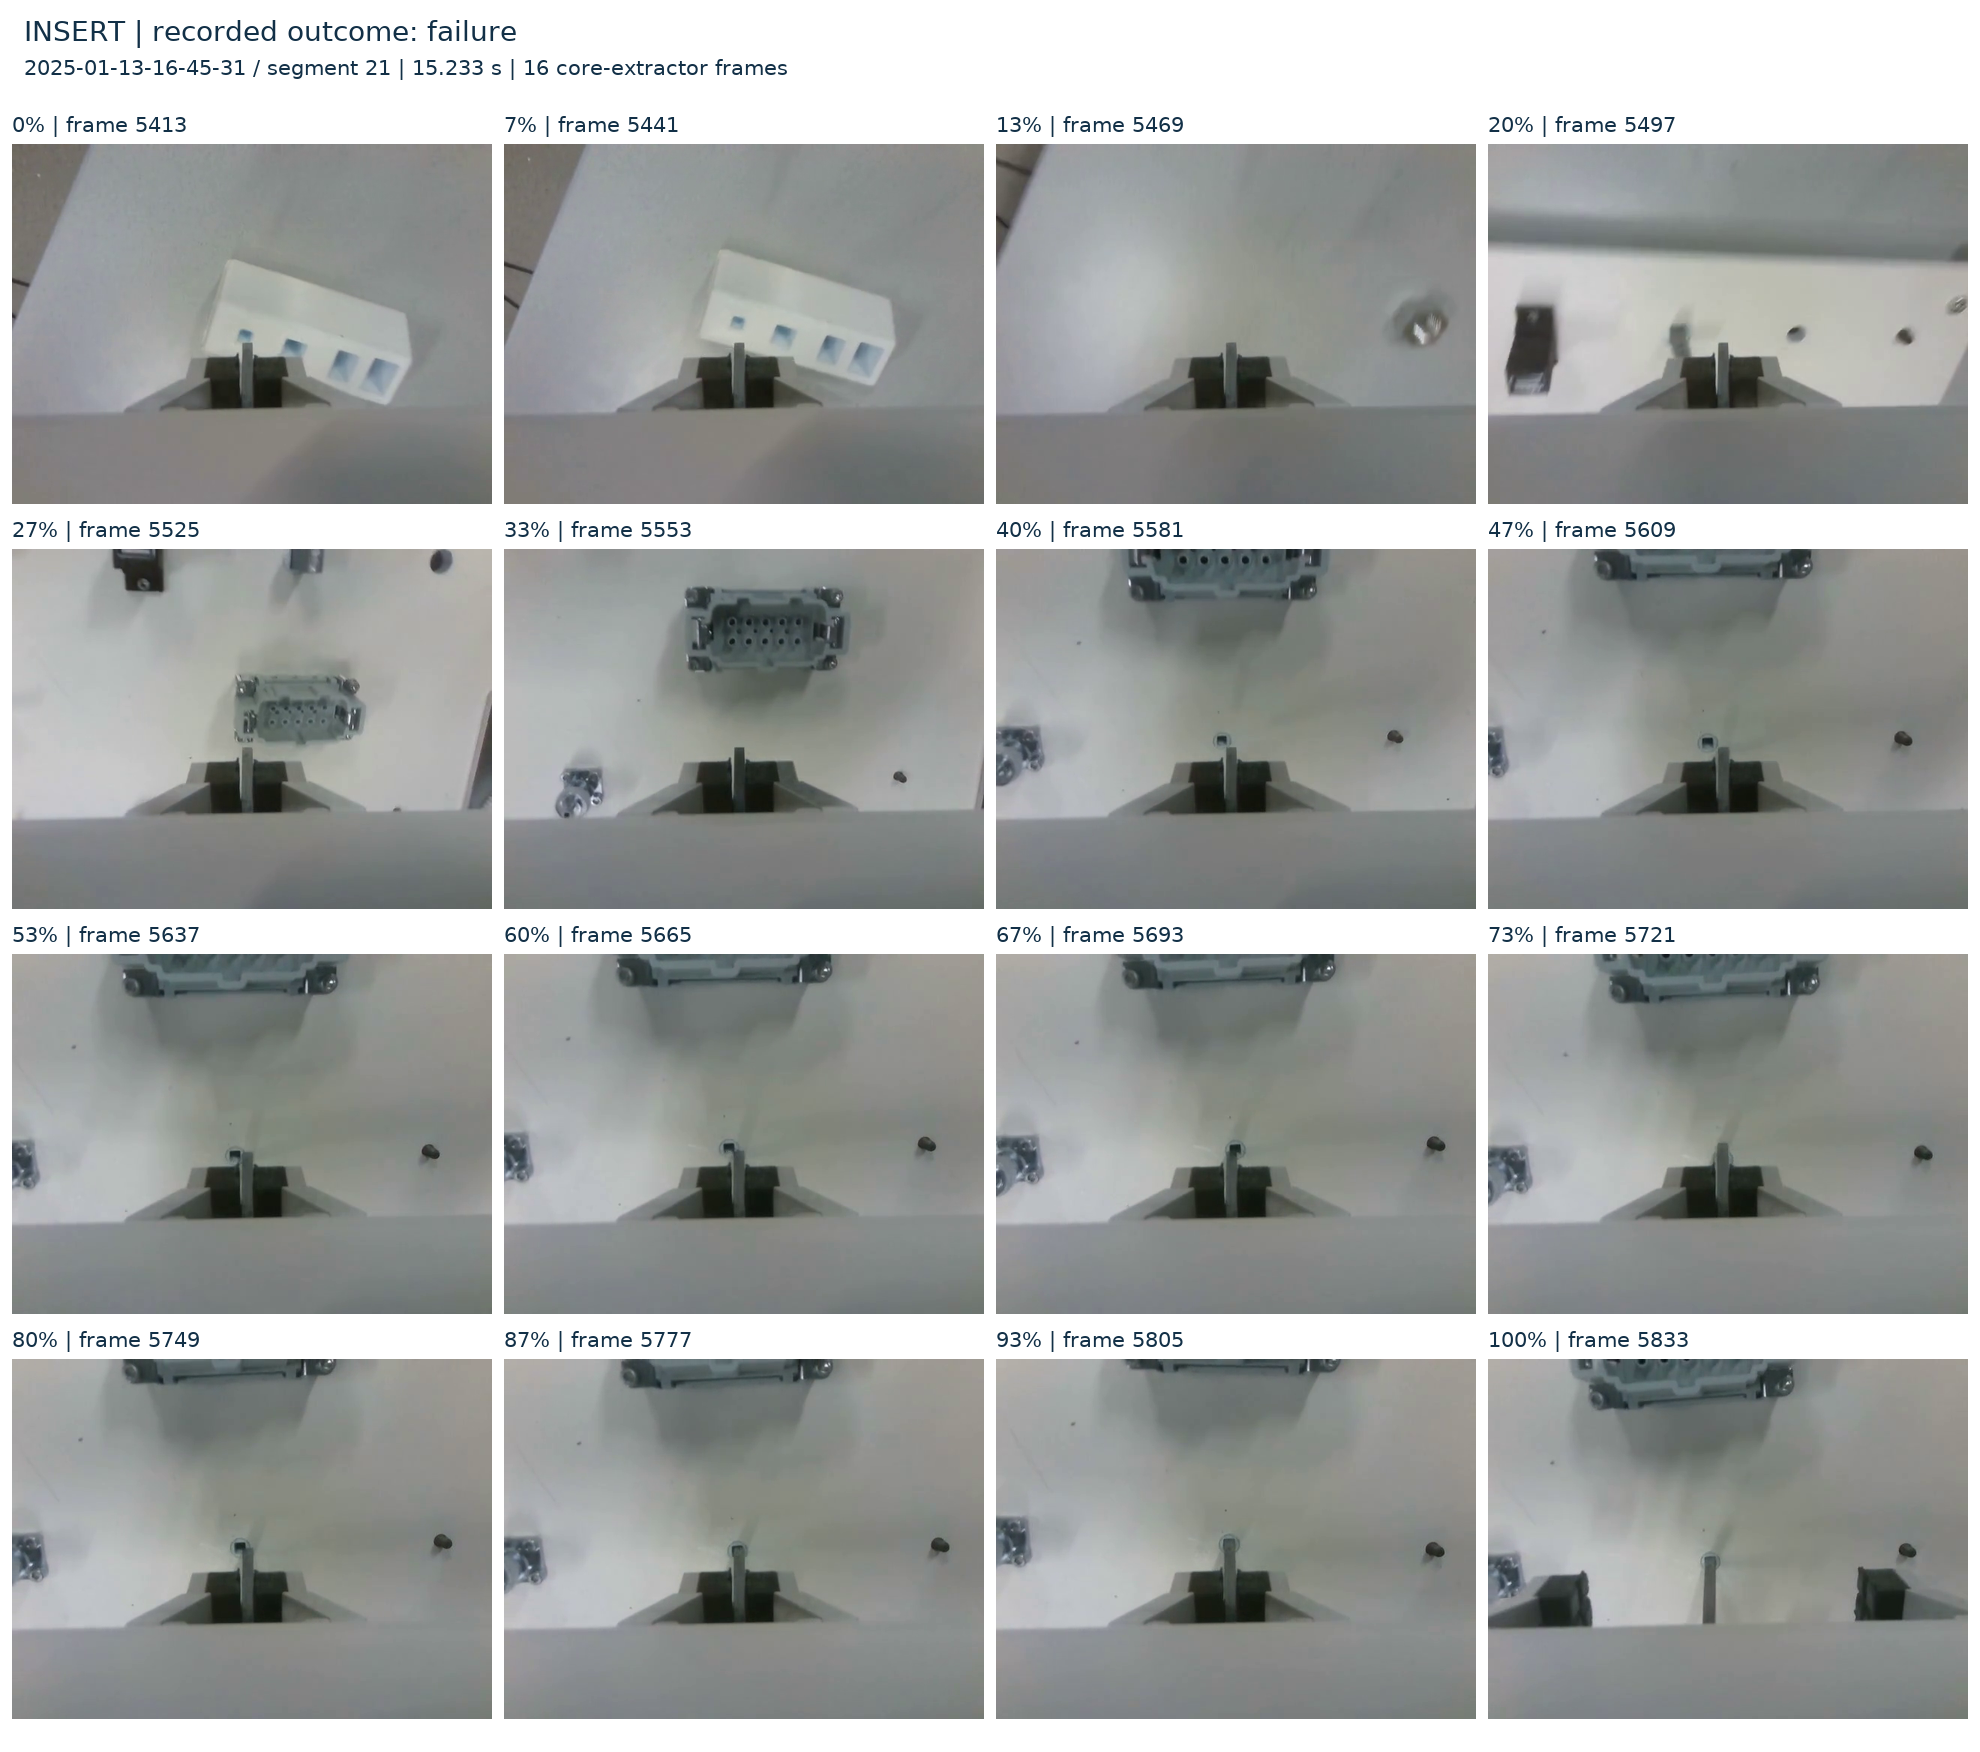
\includegraphics[width=\textwidth,height=.70\textheight,keepaspectratio]{figures/reassemble_example_frames.png}
\displaynote{The extractor selected 16 frames from recording 2025-01-13-16-45-31, segment 21 (15.233 s). The saved failure label accompanies this example. Frame selection illustrates temporal coverage. Source: Saved data-preparation example.}
\end{figure}
\ev{Illustrative frame source}{\EvidenceRef{E061}{}}
\section{Study Objectives and Research-Question Mapping}
SQ1 concerns implemented visual and temporal representations relative to engineered sensor statistics. SQ2 concerns early, late and adaptive fusion under shared recording groups. SQ3 distinguishes known missing modalities, synthetic degradation of a present modality and broader distribution shifts. SQ4 concerns the controls needed to interpret these comparisons: native labels, group separation, inner selection, calibration, paired uncertainty and computational budgets. The evaluation therefore includes simple reference predictors and a strong unimodal competitor before interpreting multimodal gains.

The task is retrospective classification of an already completed action. It is relevant to monitoring and automated inspection of industrial manipulation, but it is not a direct replication of rotating-machine damage diagnosis. The observation horizon includes the action's end. Consequently, a representation that exploits late frames can be useful here without demonstrating prediction before an unsuccessful event. The dataset paper supplies acquisition context; the retained manifests and implementation establish this thesis's specific population and task \parencite{Sliwowski2025REASSEMBLE}.\ev{Action targets and assessment cohort}{\EvidenceRef{E046}{}}

\section{Dataset Overview and Native Outcome Annotations}
The inventory contains 149 recordings; the retained common cohort contains 4,530 eligible actions from 148 recordings. A failure is one minus the native success indicator. There are 509 failures, giving positive-class prevalence 0.1124. Failure frequency differs substantially by action: pick has 98 failures in 1,190 actions; insert, 243 in 1,156; remove, 146 in 1,096; and place, 22 in 1,088. This makes action identity a substantive baseline. These filtered counts are distinct from the dataset paper's broader acquisition counts, because eligibility and task construction define the analysis population \citep{Sliwowski2025REASSEMBLE}.

The native outcome describes task success, not a spatial defect mask, severity score or verified physical root cause. One recording can contribute many actions, and actions from a recording share acquisition context. Counting 4,530 actions as independent experiments would overstate the amount of independent evidence. Recording identities are accordingly used for outer splitting and uncertainty resampling.\ev{Population and class counts}{\EvidenceRef{E046}{}}

\section{Dataset Challenges and Modality Availability}
The retained modalities are hand-camera images and machine-sensor measurements: three force channels, three torque channels, two gripper channels, seven joint-effort channels and seven joint-velocity channels. These twenty-two channels include operating state as well as direct interaction measurements. Complementarity is thus an empirical question, because both modalities may encode action identity or progress rather than independent evidence of failure.

Segment-offset and drift checks could not establish a common timing anchor for audio, so the predictive experiment excluded the audio branch. This is an alignment limitation, not a result showing that an audio model failed to learn. Similarly, seventeen object categories do not establish seventeen disjoint physical objects. The available relationship graph did not support a verified object-instance-disjoint test. The recording-disjoint split evaluates transfer between recordings. Generalization to unseen objects or sites and hardware-clock synchronization remain untested.\ev{Audio alignment and object-group feasibility}{\EvidenceRef{E044}{}}

\section{Preparation and Pre-Checks}
Preparation established a common cohort before comparing architecture outputs. Required information included native action boundaries and outcomes, valid camera correspondence, sufficient sensor coverage, and a recording-group identity. These checks support comparable inputs and prevent changing the evaluation population in response to a particular model's performance. They do not certify that every outcome label is unambiguous or that every sensor is physically calibrated.

Eligibility checks and representation choices are distinct: temporal pooling changes the view of an accepted action, whereas missing observations can affect eligibility or require a missingness policy.\ev{Preparation and common cohort}{\EvidenceRef{E046}{}}

\subsection{Cohort Construction and Exclusions}
The core analysis uses exactly 4,530 common eligible actions and retains one outcome per action. Inventory recordings and retained recordings are reported separately rather than treating the unused recording as evidence of unexplained model failure. Actions outside the four specified types or without usable required observations are outside this cohort. Exclusion manifests, rather than model-score thresholds, define eligibility.

Later studies sometimes assess only 753 of these actions. That population is the original outer-fold-zero assessment subset, containing 77 failures in 26 recordings; it is not a newly acquired independent holdout. Its prevalence, approximately 0.1023, differs from the complete cohort's prevalence. Because average precision depends on prevalence and population composition, a 753-action AP cannot be ranked directly beside a pooled 4,530-action AP as if only architecture had changed.\ev{Core cohort}{\EvidenceRef{E046}{}}\ev{Populations used in follow-up comparisons}{\EvidenceRef{E058}{}}

\subsection{Visual--Sensor Correspondence and Action Boundaries}
Sixteen distinct frames are selected deterministically at approximately uniform positions within each completed action. The selection uses the recorded action interval; it does not learn where failure begins. Sensor observations are associated with that same action and resampled to 512 normalized progress positions. These positions are not a 512-Hz sampling rate. Normalized progress enables fixed-shape fitting across different action durations while changing the temporal interpretation of features.

Checks establish manifest-level correspondence and acceptable available coverage. They do not prove sub-frame synchronization from a shared hardware clock. Boundary errors can affect both modalities jointly, and late visual information may reflect the already known outcome. The subsequent boundary review and temporal pooling experiment address parts of this problem, without converting the task into online warning.\ev{Input construction}{\EvidenceRef{E064}{}}\ev{Boundary-aware follow-up}{\EvidenceRef{E042}{}}

\subsection{Missing, Invalid, and Inconsistent Observations}
Sensor extraction requires at least 0.89 finite coverage per channel and avoids extrapolation and interpolation across long gaps. Accepted residual missing values are filled with training-partition means after channel standardization. Masks remain part of the input preparation, but the retained PatchTST configuration does not convert the observed mask into attention suppression. Passing a mask to an API and enforcing missing-token attention are therefore different claims.

Some proposed quality descriptors have limited information even on clean data. The gripper median-absolute-deviation outlier statistic is undefined for 1,562 rows and is imputed from training data; sixteen quality fields are constant. These details qualify the interpretation of a quality-aware gate: its input name alone does not establish that it receives a reliable independent quality estimate. Conversely, the deliberate complete-modality-loss experiments supply a known availability mask, which is stronger information than detecting an unnoticed hardware failure.\ev{Sensor preparation}{\EvidenceRef{E064}{}}\ev{Quality audit}{\EvidenceRef{E048}{}}

\subsection{Human Annotation Review and Its Limits}
One reviewer completed 64 selected clips. Of 59 determinate judgments, 57 agreed with the native outcome and two disagreed; five of 64 were indeterminate. Agreement among determinate cases is therefore 96.6\%, while agreement over all reviewed cases is 89.1\%. These denominators answer different questions. Sampling balanced action and label strata with recording spread rather than drawing an unstratified population sample, so neither proportion is an unbiased dataset-wide error estimate.

For action boundaries, sixty clips were acceptable, three questionable and one indeterminate; four possible presentation artifacts were also flagged. Overlapping flags identify ten unique clips requiring adjudication. A single reviewer completed the assessment. Inter-rater agreement and adjudicated outcomes are therefore unavailable. Labels, folds and model metrics consequently retain their original definitions; the review identifies specific uncertainties rather than supplying a replacement ground truth.\ev{Single-reviewer action and boundary judgments}{\EvidenceRef{E051}{}}

\subsection{Group Definitions and Split Checks}
Five outer folds hold out whole recordings, with four recording-disjoint inner folds for selection. Outer assessment populations contain 753, 964, 1,037, 906 and 870 actions; their failure counts are 77, 109, 125, 99 and 99, respectively. The corresponding recording counts are 26, 31, 32, 29 and 30. Summing the assessment rows recovers all 4,530 actions, 509 failures and 148 recordings exactly.

Within each outer training set, the visual and sensor branches supplied out-of-fold (OOF) predictions for training the logistic stacker. Each branch predicted an action using a fit that excluded its recording. During inner validation of the stacker, however, every split reused this bank. Some rows used to train the stacker could therefore come from branch fits that had seen recordings assigned to the stacker's inner validation split. This indirect dependency affects internal model and threshold assessment. It does not extend to the outer test: those recordings were excluded from branch fitting, calibration, stacker training and threshold selection. Fully independent inner validation would require rebuilding the branch prediction bank within every stacker-validation split, including repeated branch fits and calibration across all five outer folds. This additional nesting was beyond the training budget, so the outer scores evaluate the procedure that reused the outer-training bank.\ev{Dependencies in stacker validation}{\EvidenceRef{E004}{section 15.4}}

\section{Task Formulation, Model Inputs, and Shared Evaluation Protocol}
The positive class is failure. The principal ranking measure is average precision (AP), computed by the average-precision implementation rather than trapezoidal integration of a precision--recall curve. AUROC, balanced accuracy, macro-F1, failure recall and precision, Brier score and fifteen-bin equal-width expected calibration error (ECE) describe other aspects of performance. Precision--recall reporting is particularly important at the observed minority-class prevalence \parencite{Saito2015PrecisionRecall}.

Unless a later subsection states otherwise, reported core scores pool each action's outer-held-out probability across the five folds. Pooled AP is not the arithmetic mean of five fold AP values. Training-only selection and sigmoid logistic calibration use appropriate inner outputs. Hard-decision thresholds maximize inner balanced accuracy over 0.01--0.99, with ties resolved toward 0.5. Calibration and threshold selection are separate operations. Two thousand paired recording-cluster bootstrap resamples quantify uncertainty conditional on the retained fitted models; they do not refit the entire procedure or estimate all training-seed uncertainty. Nineteen structured label-shift permutations preserve recording/action structure under their conditional exchangeability assumption, giving a smallest plus-one probability of 0.05.\ev{Metrics and inference definitions}{\EvidenceRef{E046}{}}

\section{Experiment A: Unimodal Representations}
The unimodal study establishes a reference hierarchy before fusion. Class-prior, majority and action-type predictors reveal what can be achieved without detailed observations. Engineered sensor statistics are then compared with the frozen visual representation and a compact sensor Transformer. Identical retained action identifiers and recording groups prevent changes in population from masquerading as representation gains.\ev{Unimodal experiment}{\EvidenceRef{E046}{}}

\subsection{Objective and Comparison Rationale}
The unimodal comparison included simple predictors that can exploit process or sensor information beyond class prevalence. The action-type predictor controls for the large native failure-rate differences between pick, insert, remove and place. The sensor-statistics model controls for useful low-complexity descriptions of force, torque and motion. The two neural branches test different inductive biases within bounded budgets; they do not represent exhaustive optimization of all visual or time-series models.

Both neural branches improved AP over the action baseline. Their AUROC differences remained unresolved. A later test of incremental predictive value motivated the visual--sensor fusion comparison.\ev{Neural baselines and incremental fusion comparison}{\EvidenceRef{E047}{}}

\subsection{Visual Representation Configurations}
The core visual extractor loads the COCO-pretrained RT-DETR-R18vd checkpoint (\texttt{PekingU/rtdetr\_r18vd}) at the recorded revision. From the loaded detector instance, it selects \nolinkurl{wrapper.model.backbone.model}, the checkpoint's own ResNet18-vd CNN backbone, and freezes its parameters. The forward pass reads this backbone's feature maps and bypasses the hybrid Transformer encoder, detection decoder, and box heads \parencite{Zhao2024RTDETR}.

Frames are resized to $640\times640$ using bilinear interpolation, converted to RGB and divided by 255 without ImageNet mean/standard-deviation normalization. Spatial means from three scales concatenate to 896 features per frame; the sixteen frame descriptors are averaged. A frozen extractor feeds a $896\rightarrow128\rightarrow1$ ReLU/dropout head with 114,945 trainable parameters. Whole-action averaging discards temporal order. Weighted binary cross-entropy, AdamW with learning rate 0.001 and weight decay 0.001, batch size 128 and gradient clipping at one are used. Inner selection chooses five or ten epochs; outer budgets are 5, 5, 10, 10 and 5.\ev{Executed visual computation}{\EvidenceRef{E064}{}}\ev{Head and fitter}{\EvidenceRef{E065}{}}

\subsection{Statistical Sensor and PatchTST Configurations}
The statistical representation computes ten features per channel: mean, standard deviation, median, minimum, maximum, lower and upper quartiles, range, RMS and progress slope. Twenty-two channels therefore produce 220 features. A training-standardized, class-balanced L2 logistic model selects $C$ from 0.1, 1 and 10 by mean inner AP. A subsequent unweighted $C=1$ logistic sigmoid calibrates selected out-of-fold raw scores.

The neural branch is a scratch-trained Hugging Face PatchTST-style model with context $512\times22$, patch length 32, stride 16, hidden width 32, two layers, four heads and feed-forward width 64. Internal scaling is disabled; layer normalization and dropout 0.1 are used. Mean patch pooling and channel concatenation feed a 128-dimensional projection and binary head, giving 109,505 trainable parameters. The observed mask is passed but does not suppress attention in this configuration. Inner selection allows three or six epochs and chooses six in every outer fold. This is a compact adaptation of the patching idea, not a claim to reproduce all settings of the original PatchTST paper \parencite{Nie2023PatchTST}.\ev{Sensor classification architecture}{\EvidenceRef{E065}{}}

\subsection{Results and Computational Considerations}
Table~\ref{tab:reassemble-unimodal} reports pooled assessment scores. The majority predictor has AP equal to prevalence, while the action predictor improves ranking substantially. Sensor statistics are the strongest retained unimodal representation. Relative to statistics, PatchTST changes AP by $-0.1878$ with a paired 95\% interval $[-0.2314,-0.1407]$ and AUROC by $-0.0740$ $[-0.1004,-0.0469]$. Similar trainable head sizes therefore do not imply similar predictive utility.

\begin{table}[htbp]
\caption{Unimodal Predictions on REASSEMBLE}\label{tab:reassemble-unimodal}
\centering\small

\begin{tabular*}{\linewidth}{@{\extracolsep{\fill}}lrrrrr@{}}\toprule
Model & AP & AUROC & Recall & Brier & ECE\\\midrule
Majority & .1124 & .5000 & .0000 & .1124 & .1124\\
Action type & .1808 & .6851 & .7642 & .0951 & .0080\\
Sensor statistics & .4294 & .7793 & .6149 & .0804 & .0174\\
Frozen visual mean & .2307 & .6978 & .6621 & .0943 & .0070\\
Short-budget PatchTST & .2416 & .7054 & .5639 & .0937 & .0067\\\bottomrule
\end{tabular*}
\displaynote{Scores pool held-out predictions for 4,530 actions. Failure is the positive class.}
\end{table}

The AP intervals are $[.3801,.4828]$ for statistics, $[.1983,.2701]$ for vision and $[.2102,.2826]$ for PatchTST. The visual pipeline also includes video decoding and frozen CNN extraction, unlike fitting directly on compact statistics. In the retained warm-component benchmark, statistical sensors took 26.267 ms, vision 478.415 ms, F2 504.693 ms and F6 564.021 ms. These measurements used a T4, four CPU threads, three deterministic segments, sensor arrays in memory and cached compressed video; fusion times are sequential component sums. They establish a bounded practical cost difference rather than cold-start throughput or a real-time deployment guarantee. Counting only F2's three learned combination parameters would omit the branch heads and frozen visual backbone.\ev{Saved unimodal estimates}{\EvidenceRef{E046}{}}\ev{Bounded component timing}{\EvidenceRef{E043}{}}

\subsection{Interpretation and Implications for Fusion}
Visual AP exceeds the action reference by 0.0499 $[.0225,.0836]$, and PatchTST exceeds it by 0.0608 $[.0293,.0974]$. Their AUROC differences, 0.0127 $[-.0154,.0406]$ and 0.0203 $[-.0115,.0494]$, remain unresolved. These are metric-specific findings, not equivalence results. Lower neural AP than sensor statistics also does not exclude incremental information: useful errors can differ even when one standalone predictor is weaker.

The fusion experiment therefore uses the statistical sensor predictor as its reference. Each fitted fusion pipeline is compared with that predictor on the same held-out actions. The stacker also fits a new logistic map to the branch probabilities. Isolating the contribution of video to the stacker would require a sensor-only comparator with the same second fitting step. A separate follow-up tests how the training budget affects PatchTST performance.\ev{Paired unimodal and incremental fusion comparisons}{\EvidenceRef{E047}{}}

\section{Experiment B: Fusion Strategies}
Six fusion families share the cohort and recording structure: probability averaging, stacking, representation concatenation and three context-dependent gates. Their input spaces and calibration stages differ.\ev{Fusion experiment}{\EvidenceRef{E048}{}}

\subsection{Objective and Hypotheses}
The first hypothesis is that the combined visual--sensor pipeline improves held-out failure ranking relative to the retained sensor pipeline. The second is that action or quality context improves allocation between branches. These questions are distinct: a fixed map can use complementary predictions without an effective per-instance reliability estimate. The incremental comparison also changes the fitted probability map, so an improvement over sensors alone cannot isolate visual information from the benefit of an additional calibration or stacking stage. An otherwise identical sensor-only meta-calibration control was not completed. Both sensor-only and simple static fusion references are therefore needed when interpreting adaptive models.

Clean gains do not establish corruption recognition; the subsequent experiment tests frozen clean-trained models directly.\ev{Fusion questions and controls}{\EvidenceRef{E048}{}}

\subsection{Compared Architectures and Exact Fusion Formulations}
F1 averages calibrated probabilities: $p=(p_v+p_s)/2$. F2 fits a fixed-$C=1$ L2 logistic stacker,
\begin{equation}p=\sigma(b+a_vp_v+a_sp_s).\end{equation}
It has three scalar parameters. Its signed coefficients are unconstrained and do not form convex reliability weights. F3 instead projects the 128-dimensional visual representation and 220 sensor statistics to separate 128-dimensional vectors, concatenates and layer-normalizes them, and uses a hidden layer of width 32 or 64. Candidate training budgets are ten or twenty epochs.

F4--F6 use a masked softmax gate and calibrated branch logits:
\begin{equation}w=\operatorname{softmax}(h(u)+\text{availability mask}),\qquad p=\sigma\!\left(\sum_m w_m\operatorname{logit}(p_m)\right).\end{equation}
F4 receives four action indicators and two availability indicators. F5 receives thirty-six quality descriptors and availability; F6 receives all forty-two inputs. Hidden widths are eight or sixteen. The gates have no final intercept correction or post-gate calibrator. Context or quality can encode process content as well as reliability; interpreting a learned weight as causal sensor trust is therefore unsupported.\ev{Exact implemented fusion links}{\EvidenceRef{E066}{}}

\subsection{Training, Calibration, and Evaluation}
Fusion uses branch prediction banks with recording-excluded row construction and held-out outer assessment recordings. The internal bank-reuse dependency described above remains part of its selection procedure. F2 stacks calibrated probabilities, whereas F4--F6 mix calibrated logits. F2 fixes $C=1$ and has no further calibration stage. F3 uses weighted binary cross-entropy and a sigmoid calibrator; the gates use unweighted binary cross-entropy, forty epochs, learning rate 0.003 and weight decay 0.001. These differences in link, objective and calibration opportunity are part of the recipes, rather than controls that isolate adaptation alone.

Gate results average probabilities from seeds 20260927--20260929. Averaging probabilities is not equivalent to inserting averaged weights into a sigmoid. The core threshold protocol and paired recording bootstrap remain in force. These controls improve comparability but do not equalize every architecture's effective capacity, objective or calibration opportunity.\ev{Fusion training and nested banks}{\EvidenceRef{E048}{}}

\subsection{Predictive Results and Uncertainty}
F2 has AP 0.4473 and AUROC 0.7950. The paired differences for F2 minus the statistical sensor predictor were 0.0179 $[.0086,.0283]$ in AP and 0.0156 $[.0060,.0255]$ in AUROC. The Brier score difference was $-0.0020$ (95\% CI $[-.0031,-.0009]$), indicating lower probability error for F2. The ECE difference $-0.0036$ $[-.0127,.0099]$ and recall difference $-0.0039$ $[-.0255,.0163]$ remain unresolved. The more precise AP contrast is $+0.017907$ $[.008603,.028284]$. Against probability averaging, F2's AP gain is only $+0.001556$ $[-.007607,.011165]$, which does not establish a discrimination advantage. Thus the retained evidence supports a modest combined-pipeline increment over sensors, with improved probability quality on some metrics, rather than a general superiority of learned stacking over simple averaging.

\begin{table}[htbp]
\caption{Fusion Results for the 4,530 Matched REASSEMBLE Actions}\label{tab:reassemble-fusion}
\centering\small

\begin{tabular}{lrrrrr}\hline
Model & AP & AUROC & Recall & Brier & ECE\\\hline
F1 probability mean & .4457 & .7951 & .6031 & .0834 & .0355\\
F2 probability stacker & .4473 & .7950 & .6110 & .0784 & .0138\\
F3 representation fusion & .4122 & .7856 & .6385 & .0827 & .0149\\
F4 action gate & .4437 & .7815 & .6031 & .0802 & .0128\\
F5 quality gate & .4445 & .7760 & .6012 & .0806 & .0126\\
F6 combined gate & .4414 & .7755 & .5717 & .0807 & .0124\\\hline
\end{tabular}
\end{table}

All three original gates have lower AUROC than F2, with intervals excluding zero for those differences. Their AP differences remain unresolved. The AP difference for F6 minus F2 was $-0.0059$ $[-.0248,.0137]$. The failure-recall difference for F6 minus F2 was $-0.0393$ (95\% CI $[-.0649,-.0122]$).\ev{Fusion results and paired contrasts}{\EvidenceRef{E048}{}}

\subsection{Modality Complementarity and Error Analysis}
At the frozen hard-decision thresholds, both unimodal branches are correct on 2,347 actions and both wrong on 529. Vision alone is correct on 486, while sensors alone are correct on 1,168. Among 509 failures, 240 are identified by both, 99 by neither, 97 by vision alone and 73 by sensors alone. Failures detected by vision alone occurred in 61 recordings.

An oracle that always selected a correct branch would identify 410 of 509 failures, approximately 0.8055 recall. That is an unavailable truth-dependent upper reference, not an achieved fusion result or a deployable gate. Complementarity provides potential information, while learning which branch to trust from available inputs remains a separate problem. These counts describe decisions at fixed thresholds. Paired AP comparisons assess the ranking of the same actions across thresholds.\ev{Error-overlap analysis}{\EvidenceRef{E047}{}}

\subsection{Interpretation and Comparison Limits}
The core supports a small increment from the fitted combined pipeline over the retained sensor predictor. Error-overlap counts make visual complementarity plausible, but they do not identify the causal contribution of visual information separately from the additional probability map. The missing sensor-only meta-calibration control limits that attribution. F1 and F2 have similar ranking and different Brier/ECE; a calibration improvement and an information gain are not interchangeable claims.

Within the tested representations and budgets, neither intermediate fusion nor the original adaptive gates establishes an advantage over the successful static reference. This finding is architecture- and protocol-specific. The later anchored model changes the link and learns a different function class; its positive exploratory AP result is therefore compatible with the original gates' bounded negative evidence.\ev{Original REASSEMBLE fusion comparisons}{\EvidenceRef{E044}{}}

\section{Experiment C: Missing and Degraded Modalities}
The core robustness study froze the clean-trained statistical sensor and visual predictors (U1 and U2), equal averaging (F1), the stacker (F2), and the two gates using quality descriptors (F5 and F6). It perturbed one input at a time and also tested known loss of a full input stream.\ev{Core robustness study}{\EvidenceRef{E055}{}, \EvidenceRef{E049}{}}

\subsection{Robustness Questions and Tested Conditions}
The central question is whether a gate both changes allocation in the expected direction and limits predictive deterioration relative to F2. Absolute performance at high severity is also necessary: a weak clean model can show a small decline merely because little useful ranking remains to lose. An intact unimodal branch supplies a practical reference for whether fusion introduces avoidable damage.

Clean decision thresholds remain frozen during corruption. This matches a deployment in which the operator does not receive fault labels and recalibrate at every severity. Known availability masks in complete-dropout tests are an explicitly different information condition. The two sets of results measure responses to different information about the fault.\ev{Robustness contrasts and decision policy}{\EvidenceRef{E049}{}}

\subsection{Corruption Operators and Severity Definitions}
Visual operators include pixel Gaussian noise with standard deviations 0.02, 0.05 and 0.10 on the normalized scale, Gaussian blur at severities one, two and four, and removal of two, five or eight of sixteen selected frames. Sensor operators include Gaussian noise scaled by 0.1, 0.5 or 1.0 training-channel standard deviations; removal of two, seven or eleven channels; missing temporal blocks covering 10\%, 30\% or 50\% of the sequence; and six force/torque channels stuck at training medians.

Sensor statistics and quality descriptors are recomputed from the altered input, rather than retaining clean summaries beside corrupted signals. The core uses its fixed operator realization protocol. A later augmentation study averages across five stochastic test realizations. Its Gaussian-noise estimates therefore refer to a different evaluation protocol. None of these operators is direct evidence of cross-machine shift, clock drift or physical sensor recalibration.\ev{Operator implementation and severities}{\EvidenceRef{E049}{}}

\subsection{Missingness Policies and Dropout Experiments}
In the original complete-dropout test, the four evaluated fusion models used the statistical sensor probability and threshold when vision was absent. When sensors were absent, they used the visual predictor and its threshold. The evaluator received the identity of the missing stream. The core gate rejects a sample with both streams absent. The robustness report contains no empirical result for that condition. A later quality-interaction pilot marked such predictions unavailable.

A separate F6 training experiment samples visual-only dropout with probability 0.15, sensor-only dropout with probability 0.15 and both-present inputs with probability 0.70. Both-absent inputs are never sampled. Because a one-available-modality softmax has weight exactly one and the branches are fixed, its missing-case output is structurally fixed and supplies no useful gradient for improving the fallback prediction. Dropout training cannot make that output better under this architecture. Its clean AP is 0.4377, changing ordinary F6 by $-0.0037$ $[-.0085,.0003]$.\ev{Explicit fallback and dropout}{\EvidenceRef{E045}{}}

\subsection{Predictive Performance and Calibration Under Degradation}
Under strongest pixel Gaussian noise, F2 retains AP 0.3963, while F5 and F6 fall to 0.1288 and 0.1275. The intact sensor baseline remains at AP 0.4294. F2's Brier score nevertheless rises to 0.2968 and ECE to 0.4368, compared with clean sensor values 0.0804 and 0.0174. Ranking retention therefore conceals severe probability failure.

Under sensor Gaussian noise at one training standard deviation, F2 AP is 0.2222 and F5/F6 are 0.1753/0.1788, below intact vision at 0.2307. F2's Brier/ECE rise to 0.4798/0.5251. Strong blur gives F2/F5/F6 AP 0.4099/0.4061/0.4179, without a resolved general gate advantage. These conditions demonstrate that combining an intact and corrupted modality can underperform the intact branch. Detection of corruption and calibrated uncertainty remain unresolved rather than being supplied automatically by a fusion layer.\ev{Core high-severity metrics}{\EvidenceRef{E049}{}}

\subsection{Gate Behaviour and Fallback Behaviour}
No tested original gate/family combination establishes both an appropriate allocation response and a smaller decline under the study's criteria; no supported absolute high-severity AP superiority follows. A gate weight can change with a quality input without changing in a beneficial way. Conversely, a smaller performance decline from a weaker clean starting point is insufficient to establish improved reliability.

Exact missing-modality equality follows programmed fallback. It demonstrates consistent handling of known absence, while corruption recognition and useful recovery remain separate capabilities. This is narrower than training an encoder or student to retain performance after input loss, as in transferable missing-modality methods \citep{P005,P007,P016}.\ev{Gate allocation and fallback audit}{\EvidenceRef{E049}{}}

\subsection{Interpretation and Untested Conditions}
The core evidence rejects a broad claim of reliable adaptation for the tested gates. The AP, calibration and intact-branch comparisons capture different consequences of corruption. Robustness to known complete absence is largely architectural here; robustness to unnoticed corruption is empirically weak.

Natural missingness mechanisms, simultaneous partial failures, asynchronous clocks, new machines, new operating sites and prospective early warning were not established. The later augmentation study changes training exposure and tests several held-out operator families, but the same recording population and already observed core faults limit claims of independent discovery. An untested condition remains open rather than receiving a favorable interpretation from the model's name.\ev{Tested missingness and corruption conditions}{\EvidenceRef{E044}{}}

\section{Follow-up Investigations}
Three exploratory comparisons on the same cohort yielded higher average precision under their respective protocols. Last-quarter visual pooling with static stacking reached 0.4934, anchored adaptation reached 0.4683, and combining long-budget PatchTST with sensor statistics reached 0.4403. Each had its own control. The temporal-pooling study was completed separately from an earlier visual experiment that stopped after partial execution. Other follow-ups examined matched corruption exposure and visual tuning.\ev{REASSEMBLE follow-up experiments}{\EvidenceRef{E040}{}}

\subsection{Longer Sensor Training and Alternative Sensor Representations}
The longer-budget experiment retains the PatchTST inputs and architecture, permits up to one hundred epochs, and uses minimum ten epochs with patience twelve. No long-budget inner fit reaches the cap; outer budgets use rounded median inner best epochs. Against a matched short-budget control, AP rises from 0.2557 to 0.2853, a difference of 0.0297 $[.0122,.0451]$. The original short-budget experiment yielded 0.2416 AP under its own protocol.

Long training remains below statistics: AP difference $-0.1441$ $[-.1861,-.1009]$. A fixed-$C=1$ stacker combining long PatchTST and statistics reaches AP 0.4403, improving statistics by 0.0110 $[.0054,.0181]$. This combines two representations of the same sensor modality. It qualifies the original budget-dependent neural result while preserving the strong engineered baseline.\ev{Matched sensor-budget experiment}{\EvidenceRef{E040}{}}

\subsection{Alternative Visual Pooling}
The boundary-aware experiment exactly reproduces the original whole-segment mean before changing pooling. AP is 0.2556 for two halves, 0.3080 for thirds, 0.3191 for the last quarter, 0.2922 for early-plus-late and 0.2250 for an ordered GRU. The original mean is 0.2307. Last-quarter minus mean AP is 0.0885 $[.0424,.1293]$; the protocol's simultaneous lower bound across five AP contrasts remains positive at 0.0301.

This supports selected temporal aggregation changes, not a general recurrent-model advantage or an isolated causal effect of temporal order. The GRU changes capacity and inductive bias, while bin concatenation changes classifier inputs. The selected last-quarter rule exploits complete-action information. Its separate F2 follow-up reaches AP 0.4934, with the more precise value 0.493437 versus original F2 0.447299: difference $+0.0461$ $[.0260,.0632]$, and AUROC difference $+0.0403$ $[.0291,.0522]$. This is a meaningful exploratory same-cohort result after representation selection, not independent confirmation or warning before the outcome. It was not combined with the anchored adaptive gate or the same-sensor hybrid.\ev{Visual pooling definitions and paired comparisons}{\EvidenceRef{E042}{}}

\subsection{Spatial-Encoder and Backbone Comparisons}
A separate five-fold comparison tests CNN-only against CNN plus the spatial hybrid encoder, with the same sixteen frames, 4,530 actions, frozen extraction and five-epoch heads. It uses its own fitting and calibration subsets. CNN-only visual AP is 0.221644 and F2 AP 0.440764; hybrid-encoder visual AP is 0.171915 and F2 AP 0.424979, with shared sensor AP 0.420926. The hybrid-minus-CNN F2 difference is $-0.015785$ $[-0.024804,-0.005800]$. Executing more of the detector therefore worsens this particular comparison, rather than automatically improving representation quality.\ev{Matched spatial-component results}{\EvidenceRef{E039}{}}

The descriptors also differ in width: CNN multiscale pooling yields 896 features and the spatial hybrid-encoder path 768. Head size, active components and compute change with that representation. The result cannot isolate an attention effect, and the attention is spatial rather than across video time. Neither path executes the object-detection decoder. CNN-only extraction, spatial-encoder extraction, final-stage tuning and complete detector training remain distinct interventions.\ev{Architectures in the spatial-component comparison}{\EvidenceRef{E057}{}}

\subsection{Frozen Versus Fine-Tuned Visual Representations}
A matched two-epoch diagnostic uses thirty-two frames for both frozen and final-stage-tuned arms across the full 4,530-action cohort. It covers two seeds, with seventy-five newly executed and twenty-five reused fits. Epoch matching does not imply compute matching. Its fixed sensor recipe has pooled AP 0.4208, distinct from the core selected-$C$ baseline's 0.4294.

For seed 42, visual AP changes from 0.2227 to 0.2306, but the difference 0.0079 has interval $[-.0173,.0332]$; F2 changes from 0.4394 to 0.4386. For seed 20261023, visual AP changes from 0.2168 to 0.2005, and F2 from 0.4352 to 0.4324. The corresponding paired intervals include zero. These results do not identify a unique cause for the absence of a fusion gain, such as calibration or out-of-fold mismatch; two seeds also do not fully characterize seed variability.\ev{Matched two-epoch diagnosis}{\EvidenceRef{E062}{}}

The later twenty-epoch visual cap completes twenty inner and five outer fits for seed 42. Pooled visual AP is 0.3121, while mean fold AP is 0.3086. The additional fifty fits for two more seeds are deferred; their absence is not a failure of the twenty-five completed fits. Twenty-epoch F2 was not executed because its controller expected the larger bank. A current checkpoint validator's twenty-five-source-epoch requirement conflicts with the twenty-epoch donor; that is an eligibility/configuration conflict, not evidence of failed training.\ev{Completed twenty-epoch fits}{\EvidenceRef{E059}{}}

The hundred-epoch pilot restarts both arms from pretrained weights with fresh heads, rather than continuing the twenty-epoch run. Both arms execute one hundred epochs and select epochs fourteen (frozen) and forty-seven (full). On the same 753-action assessment subset, visual AP is 0.1938/0.2126 and F2 AP 0.3350/0.3491. Full-minus-frozen F2 AP is 0.0141 $[-.0008,.0291]$, leaving the difference unresolved. Restricted historical F2 is 0.3672 on these same rows; its full-cohort AP is not the relevant comparator.\ev{Matched pilot assessment cohorts}{\EvidenceRef{E058}{}}

\subsection{Adaptive-Fusion Extensions and Matched Controls}
Anchored adaptation preserves the successful F2 link and learns bounded adjustments:
\begin{equation}p=\sigma\!\left(b+\sum_m a_m[1+\tanh(h_m(u))]p_m\right).\end{equation}
The adaptive network is $42\rightarrow16\rightarrow2$ with zero final-layer initialization; a two-parameter constant adjustment is a matched control. AP reaches 0.4683, improving the matched anchor by 0.0210 $[.0015,.0419]$ and the constant adjustment by 0.0226 $[.0036,.0432]$. AUROC gains remain unresolved; recall falls and ECE rises relative to the anchor. Threshold differences also prevent treating its hard decisions as identical to historical F2. This is evidence for a particular exploratory function class, not retrospective success of F6.

Matched augmentation uses 50\% clean, 25\% pixel-noise and 25\% sensor-noise training views, recomputing quality without a supplied fault identity. The principal adaptive-minus-static contrast over six seen-family conditions is AP $+0.0097$ $[-.0034,.0228]$, unresolved. Strong blur gives adaptive AP 0.3968 versus static 0.4256; eleven dropped channels give 0.2128 versus 0.2924. Sensor Gaussian noise at one training standard deviation favors augmented adaptation, 0.2081 versus augmented static 0.1749, but clean-trained F2 is 0.2246 under this later realization protocol. These selective wins do not establish general robustness, and none of the clean noninferiority claims passes the specified 0.01 margin.\ev{Anchored and augmented controls}{\EvidenceRef{E040}{}}

A later observable-quality pilot uses the selected frozen16 recipe on 753 actions, with 77 failures in 26 recordings. Its historical static clean AP is 0.307929; the changed branch, training and calibration recipe distinguishes this value from the restricted original F2 and the hundred-epoch screen. It matches augmentation exposure across three heads: static A, additive-quality B and probability--quality interaction C. All use 3,777 OOF parent actions and 11,331 augmented rows, weighted 0.50 clean, 0.25 visual fault and 0.25 sensor fault per parent. Eight quality proxies enter the relevant models; A, B and C have 3, 11 and 27 parameters. C has unrestricted interaction and direct quality coefficients, rather than convex reliability weights.

The primary mean AP across declared Gaussian conditions is 0.253996 for A, 0.237360 for B and 0.257009 for C; clean AP is 0.307397, 0.292965 and 0.312168. C minus A is $+0.003012$ $[-0.026711,+0.032165]$ for the primary mean and $+0.004771$ $[-0.034258,+0.044544]$ clean. Neither robustness superiority nor clean preservation at the pilot's zero-loss margin is established. B minus A deteriorates by $-0.016636$ $[-0.030676,-0.002429]$ in a secondary contrast on the primary metric. The primary average covers repeats, severities and two Gaussian families; it is not AP computed after pooling repeated versions as independent subjects. Complete absence routes all heads identically to the survivor, while both absent yields unavailable predictions. Quality can encode action content as well as error risk, and the different capacities plus absent quality-only/content-matched controls leave the reliability mechanism unresolved.\ev{Augmentation-matched quality-interaction results}{\EvidenceRef{E038}{}}

\subsection{Resource-Constrained Screens and Their Interpretation}
The hundred-epoch pilot uses mutually disjoint roles: 1,752 training, 419 validation, 686 calibration, 920 inner-bank and 753 assessment actions, summing to the common 4,530 population. Their recording counts are 60, 15, 19, 28 and 26. Saved prediction action identifiers take precedence over a stale metadata field listing inner-bank recordings as assessment recordings. This correction changes interpretation of provenance, not the saved scores.

The full hundred-epoch arm records about 23.96 training hours and 25.82 active process hours. The twenty-epoch cap records about 126.23 training hours across twenty-five fits; 137.47 hours includes validation/inference. Different accounting units and populations prevent treating these totals as intrinsic model costs. Removed derived caches also make a cold reproduction differ from historical cached timing. The completed subset screen supplies a bounded paired comparison, while five-fold or multi-seed performance requires the corresponding predictions.\ev{Measured training and process times}{\EvidenceRef{E060}{}}\ev{Sample allocation by fitting role}{\EvidenceRef{E058}{}}

\section{Study Synthesis and Remaining Questions}
The clearest result was the improvement in failure ranking from sensor statistics alone to the logistic stacker. The paired comparison with equal averaging remained inconclusive. Without a sensor-only model given the same second-stage calibration, the gain cannot be attributed to the camera alone. Outer-test recordings remained independent of fitting and threshold selection, although reuse of the outer-training OOF bank limited independence during inner stacker validation. The original adaptive gates showed no general advantage. When absence was known, routing returned the surviving branch's prediction. Performance under corruption showed why detecting an unreliable stream that is still present is a separate problem.

The three favorable follow-ups changed different parts of the pipeline. Last-quarter pooling used the end of the completed action. Anchored adaptation improved ranking but reduced recall and increased calibration error relative to its anchor. Longer PatchTST training improved the temporal sensor predictor but left it below sensor statistics alone; the two sensor representations performed better together. No run combined the three changes. Choosing components after comparing their results on the same recordings would compound selection bias: the choices could reflect idiosyncrasies of that cohort. A joint pipeline would need to be fixed in advance and evaluated on untouched recordings. The augmentation-matched and quality-interaction comparisons left their primary robustness contrasts unresolved. Generalization to natural failures and shifts, independently adjudicated labels, new seeds and predictions made before action completion also remains open.

\chapter{MSM Case Study: Dataset Adaptation and Evaluation Feasibility}
\label{ch:msm}

\section{Motivation and Intended Comparison}
In MSM milling, the logistic sensor model ranked abnormal intervals more accurately than the stacker (F2) that combined its predictions with video. Both models predicted the same labelled intervals under the same grouping rules. Moving from assembly to milling changed the measurements, prediction interval and target.

The study connects the original questions in a controlled sequence. The frozen CNN and interval statistics test a lightweight representation choice (SQ1); averaging, original F2 and supplementary quality gates test fusion alternatives (SQ2); controlled input stresses and explicit absence fallbacks address a bounded part of robustness (SQ3). Target semantics, grouped assessment, probability quality and the distinction between software feasibility and predictive value address SQ4. None of these comparisons establishes early warning before an abnormal cut or transfer without target-domain fitting.

The pretrained-initialization comparison covered three fixed training seeds and the specified target, grouping and corruption conditions. An initial development run tested the implementation on a small sample. Performance estimates came from the subsequent held-out intervals that met the timing and input-coverage criteria.\ev{MSM experimental design}{\EvidenceRef{E079}{}}

A close manufacturing comparator illustrates why the unimodal reference is essential. The tool-wear study in \citet{P045} combines post-pass tool photographs with acoustic information and reports its proposed MAE below a visual baseline, while other multimodal architectures perform substantially worse than that same visual baseline. Its wear-regression task, observation schedule and incompletely reported tool-split coverage differ from MSM. It motivates testing the contribution of a second stream; it does not supply a transferable numerical expectation of improvement.

\section{Dataset Overview and Target Semantics}
The source dataset combines laboratory and industrial metal-cutting observations \citep{Kim2026MSM}. It is a data descriptor, rather than a published unimodal-versus-fusion benchmark. Its streams have different sampling and refresh rates, and the smartphone camera is available only in the laboratory material. The evaluated release is the pinned Kaggle version~2 \citep{MSMKaggle2025}. The retained laboratory material covers VM20i and VMX30Ui; the industrial VF10 component is outside this visual comparison because it does not supply the corresponding video. The source overview describes 56 laboratory experiments. Membership in that inventory is distinct from admission to the final paired cohort.

Native labels distinguish stable normal cutting, intervention-worthy abnormal cutting, and stable cutting with a defective tool. Their values are respectively 0, 1 and 2. The primary binary outcome is label~1 against labels~0 and~2. A negative outcome therefore means stable cutting under this definition; it does not certify a healthy tool. Expert annotation uses process behavior, sound and measurements, so the label is an observed process judgment rather than an independently instrumented future-failure endpoint. Relabeling every defective-tool interval as abnormal would change the task. The study instead repeats the pipeline after excluding label~2 and retains that as a distinct target sensitivity.\ev{MSM target definition}{\EvidenceRef{E074}{}}

Of 2,512 native labeled intervals, 1,895 satisfy the joint video and numerical-input requirements, including 336 positives. The remaining 617 retain their original labels and explicit exclusion reasons. One prediction refers to one completed cutting interval. Neither the whole interval nor its final label is shortened into a prediction horizon that would establish advance warning.

\section{Dataset Challenges}
Milling video can show the machine and process context while coolant, enclosure geometry and occlusion conceal the tool--workpiece interaction. Successful decoding is therefore insufficient evidence that the labeled abnormality is optically observable. A visual classifier may respond to operating context, lighting or experiment-specific appearance rather than the underlying cutting event. The substantial visual training--assessment gap reported below is compatible with this concern, but does not identify its cause.

The machine stream is also an observation of the process rather than direct, instantaneous ground truth. Aggregated electrical, load and vibration-related measurements can describe an interval while smoothing short events. Their timing and update cadence limit any claim about event onset or control latency. Group identity creates a further difficulty: experiment folders provide a useful split boundary, but they are not verified identities for physical tools, workpieces or sessions. These limits motivate both the technical gates and the stricter grouping sensitivities.\ev{MSM validation limits}{\EvidenceRef{E075}{}}

\section{Preparation and Pre-Checks}
Preparation admits examples only when both modalities meet a fixed input contract. The dominant exclusion is lack of validated acoustic timing support, followed by rejected or insufficient alignment and numerical gaps. These are technical exclusions, not removals based on model correctness. The exclusion record identifies intervals removed before modelling. Successful decoding alone does not establish that an anomaly is visible.

\subsection{Video Timing and Interval Correspondence}
The final adapter reuses the corrected Stage~2/5 acoustic calibration rather than fitting timing offsets against outcome labels. Its convention is video time equal to sensor time plus the accepted offset, within the region supported by the calibration. A documented correction matters here: VMX9 uses an offset of $+49.73$~s; the rejected $+16.04$~s alias is not an interchangeable alternative. Treating the two alignments as equivalent would change which visual evidence accompanies each native interval.

Cuts use half-open intervals and uncertainty guards. Each admitted interval has sixteen ordered, distinct native frames with source timestamps and content identities. The assessment concerns the accepted support, not every point of the original recording. An accepted offset supplies a defensible correspondence under the recorded calibration; it does not prove hardware synchronization or eliminate residual timing uncertainty.\ev{MSM timing and alignment checks}{\EvidenceRef{E075}{}}

\subsection{Visual Coverage and Geometry}
The frozen recipe corrects the source sample aspect ratio of $3{:}8$ and uses aspect-preserving, centered black letterboxing to $640\times640$. This preserves geometry instead of stretching narrow process views into a square. Sixteen interval frames pass through the same CNN, and spatial and temporal means produce one interval representation. Frame order is retained in provenance but is not learned by the mean-pooling model.

At least sixteen distinct native frames are required; repeating a short clip to reach the nominal frame count is not accepted as additional temporal coverage. Later stress conditions alter actual image content before feature extraction. Neither the common crop nor a displayed context view is a detector box, a tool annotation, or a verified abnormal region. The derived galleries support examination of the evidence and errors; they do not replace independent frame-level annotations.\ev{MSM visual input contract}{\EvidenceRef{E068}{}}

\subsection{Sensor Coverage and Measurement Interpretation}
The evaluated numerical input comprises fifteen MTConnect channels: power, spindle speed and load, feed rate, axis loads, and the supplied RMS-related channels. Six channel-major statistics---mean, population standard deviation, RMS, minimum, maximum and peak-to-peak---yield ninety values per interval. The channel names and measurement semantics remain those of the release; they are not recast as a new calibrated force signal.

Numerical support must contain at least five finite rows, with no gap greater than $0.5$~s including interval edges. The pipeline neither interpolates an unsupported gap nor substitutes an accelerometer branch. Means, standard deviations, imputation values and corruption scales that require population estimation are fitted only within the appropriate training partition. This prevents the assessment distribution from influencing the numerical normalization, while leaving the source stream's aggregation and latency limitations intact.\ev{MSM numerical coverage}{\EvidenceRef{E075}{}}

\subsection{Class Support and Independent Groups}
The primary cohort has 45 nominal experiment groups, 17 containing positives, seven machine/date proxies and five calendar dates. Every actual fitting, out-of-fold and assessment partition must contain both classes. Table~\ref{tab:msm-support} records the positive/total assessment support for all six target/grouping protocols. The folds within a protocol partition its admitted cohort; the six protocols are sensitivities on related observations, not six independent datasets.

\begin{table}[htbp]
\caption{Class Counts in the MSM Assessment Folds}\label{tab:msm-support}
\centering\small

\begin{tabular}{lrrr}\hline
Target and grouping & Fold 0 & Fold 1 & Fold 2\\\hline
Primary, experiment &157/567&37/730&142/598\\
Primary, machine/date &38/468&95/664&203/763\\
Primary, calendar date &157/422&99/689&80/784\\
Exclude label 2, experiment &138/712&122/429&76/629\\
Exclude label 2, machine/date &38/447&95/641&203/682\\
Exclude label 2, calendar date &99/645&157/341&80/784\\\hline
\end{tabular}
\displaynote{Each cell gives the number of positive intervals divided by the total number of intervals. Label~1 is positive.}
\end{table}
\ev{MSM complete split support}{\EvidenceRef{E069}{}}

Experiment and date identifiers serve as proxies for physical independence. Repeated tool or workpiece use across dates remains unresolved. The additional DOWN-only, label-2-excluded comparison fails the fixed class-support requirement. The split seeds and fold counts were fixed, leaving that comparison without an estimate. Direction-specific held-out summaries are descriptive and cannot isolate a causal effect of cutting direction.

\begin{figure}[p]
\caption{Paired Camera Frames and Sensor Measurements for an MSM Milling Interval}\label{fig:msm-example}
\centering
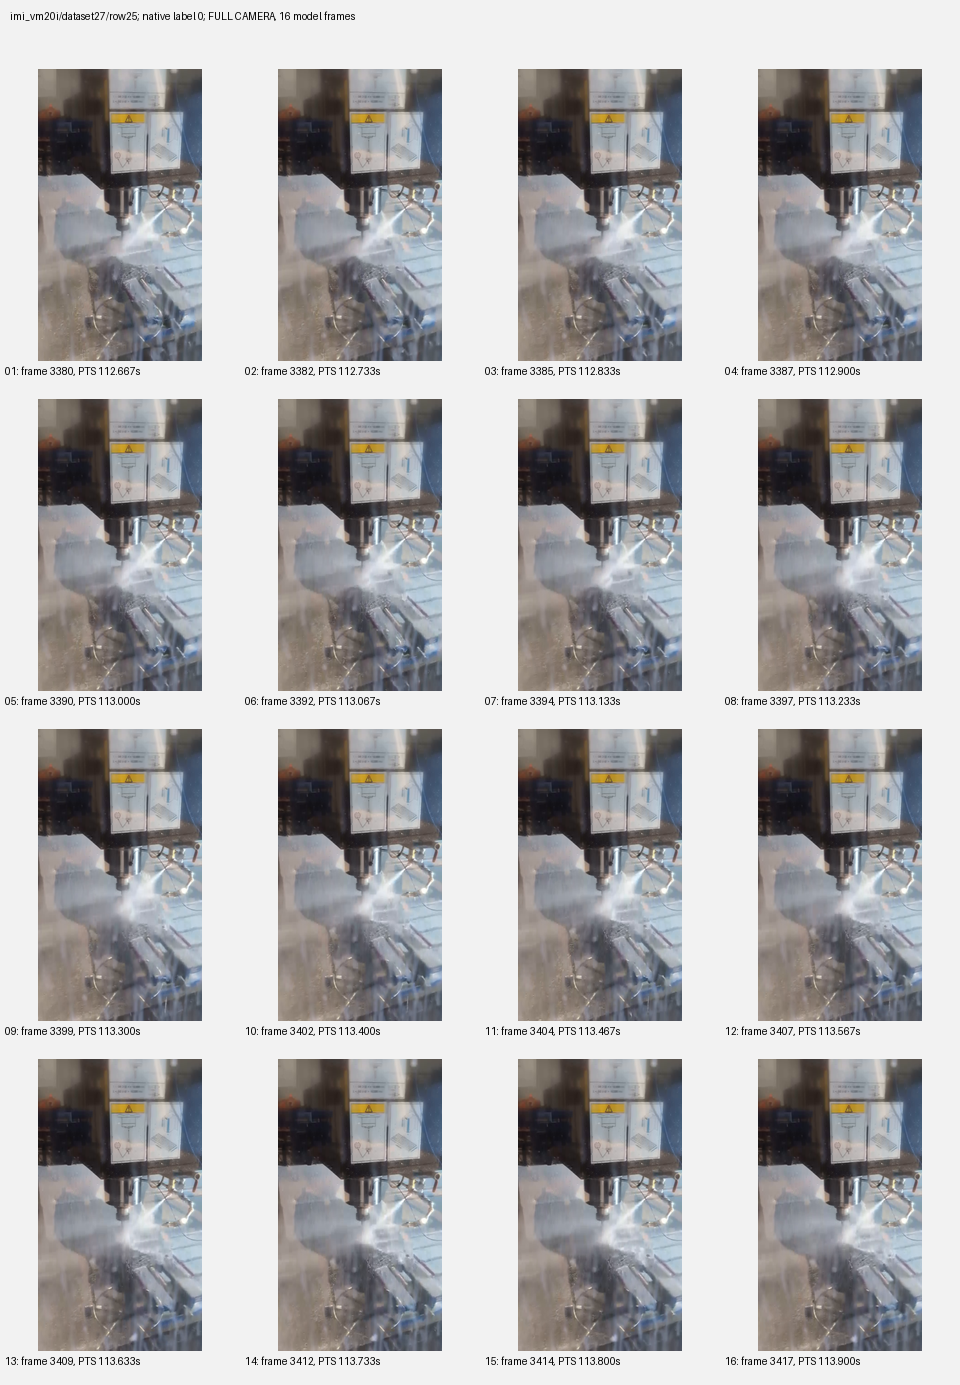
\includegraphics[width=\textwidth,height=.37\textheight,keepaspectratio]{figures/msm_example05_frames.png}\par\vspace{3mm}
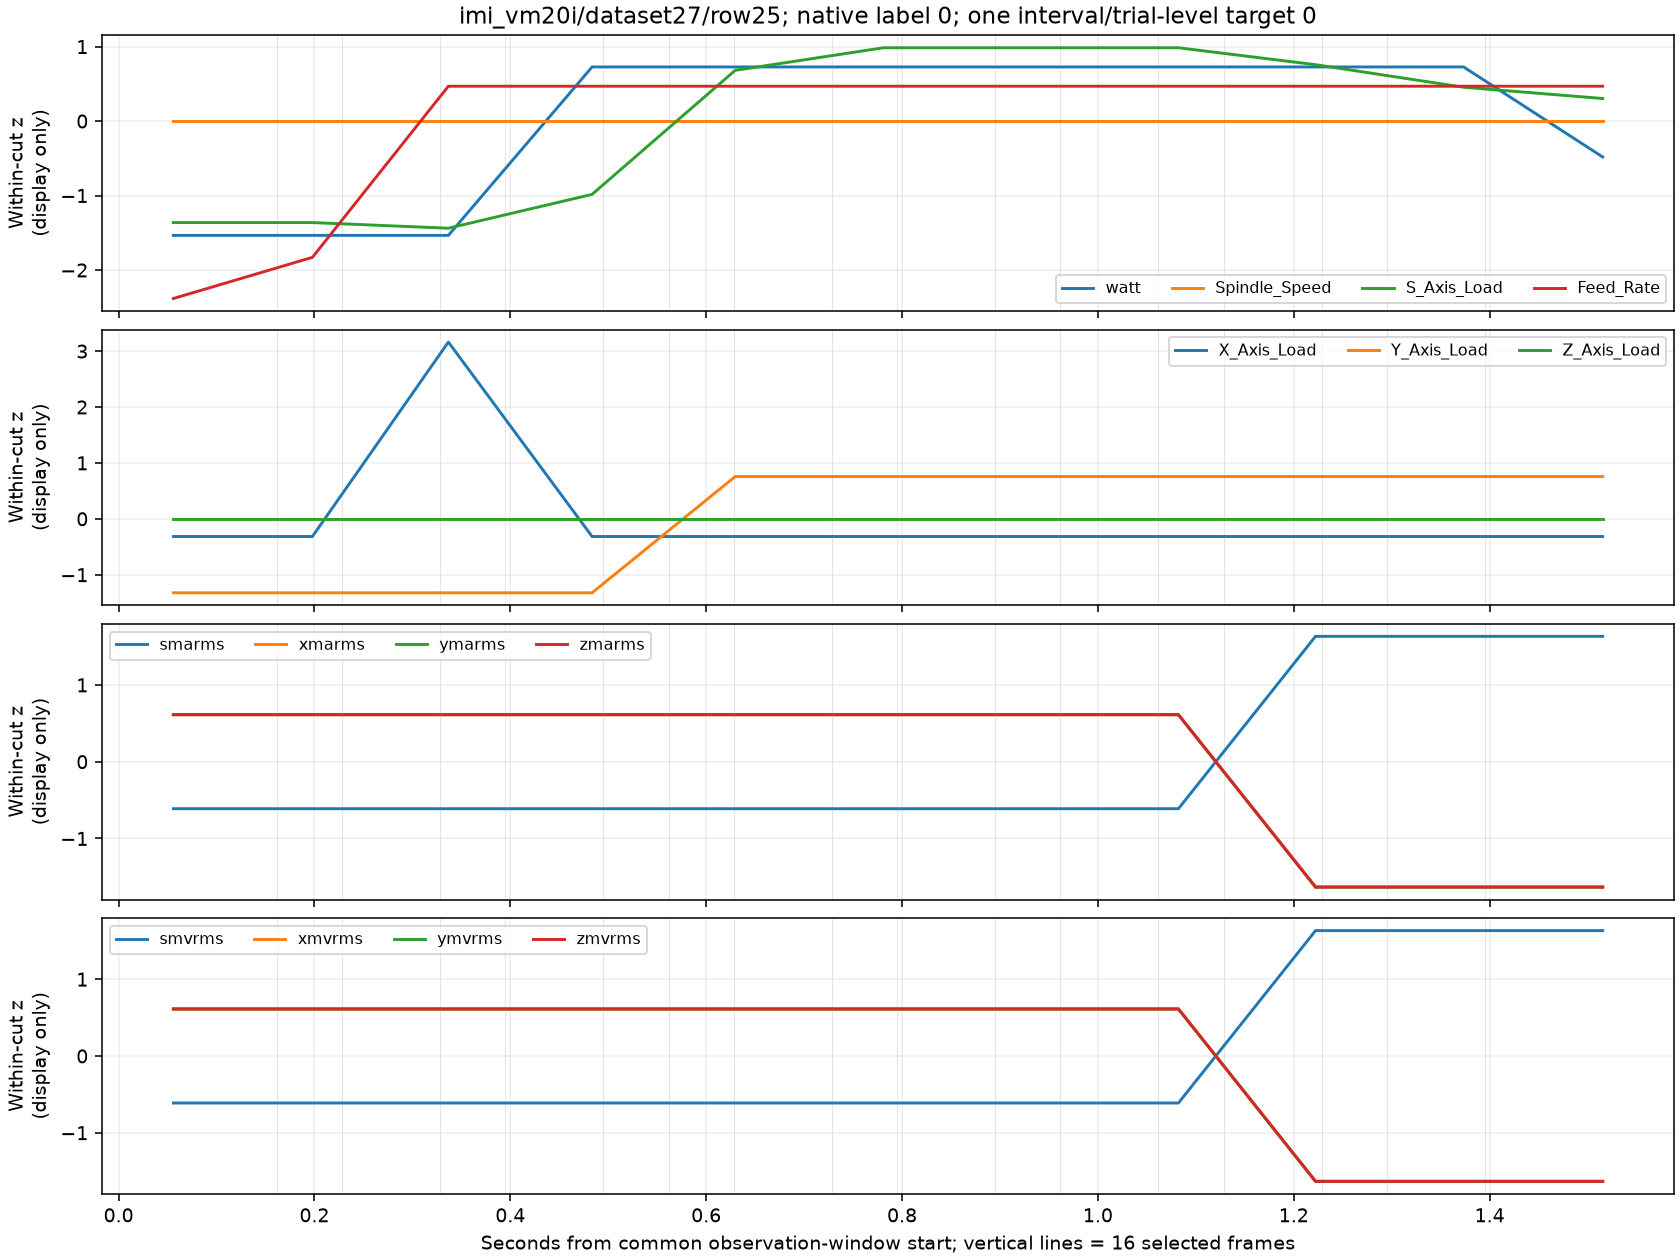
\includegraphics[width=\textwidth,height=.31\textheight,keepaspectratio]{figures/msm_example05_sensor.png}
\displaynote{The 16 frames and time-aligned MTConnect traces cover interval \texttt{imi\_vm20i/dataset27/row25}, pair P03, at 112.405--113.941~s. The recorded label is 0 (stable normal). Within-interval $z$ scores scale these curves for display. The fitted model used training-only normalization and assigned one prediction to the whole interval.}
\end{figure}
\ev{Illustrative input and identity source}{\EvidenceRef{E071}{}, \EvidenceRef{E072}{}, \EvidenceRef{E073}{data row 5}}
\section{Architecture Reuse and Dataset-Specific Adaptations}
The pretrained condition (P) used the ResNet18-vd CNN backbone inside the RT-DETR-R18vd checkpoint \citep{Zhao2024RTDETR}. The extractor stopped at the CNN feature maps, before the hybrid Transformer encoder, detection decoder, and box heads. Spatial means from the last three maps yielded 896 features per frame. Averaging across sixteen frames gave one vector per cutting interval. With the backbone frozen, a newly fitted $896\rightarrow128\rightarrow1$ head with ReLU and dropout~0.1 supplied the target prediction. It had 114,945 trainable parameters.

The numerical branch is a fresh balanced L2 logistic regression on the ninety statistics, with $C=1$. A separately fitted histogram gradient boosting model provides the stronger sensor control. It is essential to keep that control separate: F2 consumes the logistic branch, not the HGB predictions. Averaging combines the two branch probabilities without a fitted fusion parameter. Original F2 is a newly fitted unweighted L2 logistic model on visual and sensor probabilities generated out of fold. No source failure head, scaler, calibrator or fusion coefficient is transferred.\ev{MSM executed composition}{\EvidenceRef{E077}{}}

The clean and augmented quality gates are additional comparisons. They reuse a small softmax gate over branch logits, with label-free image-quality summaries, numerical variability, missing-channel fractions and availability flags. These summaries may encode process context as well as degradation. A changing allocation therefore is not a calibrated estimate of modality reliability. This matters because a reliability-aware fusion argument requires a quality proxy that actually predicts error, rather than a proxy that merely changes with the input \citep{Zhang2023QMF}. QG-clean uses clean OOF views. QG-aug sees clean views plus seven predefined lowest-severity corruptions, while F2-aug is the exposure-matched static control. Clean fitting, corruption exposure and quality conditioning remain separate interventions.

R denotes a different question: initialization from a specifically completed REASSEMBLE-learned CNN. The exact canonical source required by MSM's gate was unavailable in the inspected evaluation, so that condition remains unmeasured. This does not contradict the P completion or the later, differently specified ViFailback donor study. Architecture reuse, generic pretraining and transfer of task-learned weights retain separate provenance.

\section{Implementation Checks and Bounded Development Runs}
The bounded development exercise was an engineering check: its two-epoch, at-most-24-interval design restricted head updates and CNN frame forwards and prohibited outer-assessment predictions. It could expose shape, gradient, memory or reload errors, but could not estimate generalization. Generalization was assessed in the subsequent evaluation on held-out intervals.

The saved implementation audit checks planned cases, source identities, native assessment units, model budgets and checkpoint reloads. It also refits the fixed F2 estimator from saved clean OOF probabilities and reports zero coefficient discrepancy. The CNN cache check reports maximum difference zero on an outer-training-only example. These support consistency of the saved procedure and its outputs. Their scope is narrower than reproduction of stochastic training: exact reload and metric recomputation cannot alone certify that every training step would recur in another environment.\ev{MSM implementation and reproduction scope}{\EvidenceRef{E078}{}}

\section{Evaluation Protocol and Conditions Without Estimates}
The completed matrix uses three outer and two inner StratifiedGroupKFold partitions, fixed split seeds and training seeds 42, 123 and 20261023. Inner fits produce branch OOF probabilities for learned fusion; outer assessments remain excluded from fitting. The six target/grouping protocols yield 54 completed case records. The 54 cases include different folds and seeds from overlapping protocols.

The main visual head runs for ten fixed epochs and the gate for forty. The assessment uses a fixed threshold of 0.5, with no assessment-selected epoch or fitted primary calibrator. Scikit-learn computes average precision as a weighted mean of precision values, with each weight equal to the increase in recall \citep{Pedregosa2011ScikitLearn}. This differs from trapezoidal integration of the precision--recall curve. F2 denotes the fusion model in this study. Primary results pool the disjoint outer predictions separately for each seed, then summarize the three APs. An arithmetic mean of fold APs answers a different question because fold prevalences and cross-fold score scales differ.

Conditions with a missing source checkpoint, inadequate class support or insufficient temporal coverage yielded no estimate. The results below cover the conditions that met the original criteria.\ev{MSM fixed evaluation protocol}{\EvidenceRef{E070}{}}

\section{Findings, Limitations, and Implications}
On intact inputs, F2 had lower AP than its logistic sensor component at all three seeds. The mean paired difference was $-0.071737$ (Table~\ref{tab:msm-clean}). F2 ranked abnormal intervals more accurately than the visual branch or equal averaging. Sensor HGB had the highest mean AP of the models compared.

\begin{table}[htbp]
\caption{MSM Prediction Performance With Intact Inputs}\label{tab:msm-clean}
\centering\small

\begin{tabular}{lrr}\hline Model&Mean AP&Seed SD\\\hline
Visual&0.298901&0.010853\\
Sensor logistic&0.828616&0.000000\\
Sensor HGB&0.901299&0.000000\\
Averaging&0.735594&0.015942\\
F2&0.756879&0.011082\\
F2-aug&0.760170&0.009783\\
QG-clean&0.837418&0.013389\\
QG-aug&0.826521&0.016168\\\hline
\end{tabular}
\displaynote{Entries summarize pooled average precision across three fixed seeds as the mean and sample standard deviation.}
\end{table}
\ev{MSM primary results}{\EvidenceRef{E076}{}}

Logistic sensing had higher mean AP than F2 in all six prespecified protocols. Excluding label~2 and grouping by calendar date gave 0.521826 for F2 and 0.891656 for logistic sensing. That sensitivity analysis changes the target. Under the primary definition, pooled prevalence was $336/1895=0.177309$ and outer-fold prevalences ranged from approximately 0.051 to 0.277. The fold-specific training-prior baseline had pooled AP 0.145395 because the fitted prior could vary across folds.

The paired 95\% calendar-date bootstrap interval for F2 minus logistic sensing was wholly negative, $[-0.100356,-0.051477]$. It used five date clusters, held fits and split assignments fixed and could not account for unidentified equipment reuse. QG-clean averaged $+0.008802$ AP above logistic sensing, with one negative seed and an interval of $[-0.097085,+0.056426]$. The interval admits gains and losses and leaves equivalence unresolved.\ev{Milling results across evaluation protocols}{\EvidenceRef{E081}{}}

At the highest sensor-noise level, QG-aug reached 0.298636 mean AP, close to intact vision at 0.298901. F2 reached 0.206863 and noisy sensor HGB reached 0.606157. Under the strongest image blur, QG-aug achieved 0.682784, below F2 at 0.771420 and intact logistic sensing at 0.828616. The comparison therefore depends on which stream deteriorates and which predictor remains available. The tests also covered brightness and contrast changes, occlusion, frame omission, zeroed channels and explicitly missing channels.

Whole-modality absence invokes a separately programmed surviving-branch fallback: 0.828616 AP without vision and 0.298901 without sensors. Equal fallback scores across fusion methods are imposed behavior, not adaptive recovery learned from data. Differences in augmentation exposure between a gate and its static control would confound the effect of quality conditioning.\ev{MSM input perturbation and fallback results}{\EvidenceRef{E080}{}}

For seed~42, F2 had lower AP than logistic sensing but a lower Brier score (0.056091 versus 0.061724) and higher F1 (0.820438 versus 0.811268). QG-clean had higher AP than F2, a worse Brier score of 0.064406 and a lower F1 of 0.786421. Thus the ranking comparison favored logistic sensing, whereas probability error and fixed-threshold decisions favored F2 for this seed. The relative performance of the gates depended on the input condition.

The visual model ranked held-out intervals poorly despite a much stronger training result. Inadequate features, limited event visibility, residual alignment error and experiment-specific appearance could each contribute. Independent annotations of event visibility and a matched representation comparison on the same groups would help distinguish these explanations.

\chapter{ViFailback Case Study: Application to a Further Dataset}
\label{ch:vifailback}

\section{Motivation and Replication Objectives}
On held-out ViFailback manipulation tasks, the logistic sensor model ranked episode outcomes more accurately than the fitted combination of video and sensor scores. The dataset provides three camera views and robot observations for complete episodes \citep{Zeng2026ViFailback}. The study compared the two branch predictions and their combination on the same tasks (SQ1 and SQ2). A separate comparison isolated the choice between a generic frozen visual encoder and one initialized from a REASSEMBLE checkpoint, with a new prediction head fitted in each case.

The primary replication contrasts original frozen vision, logistic sensing, averaging and F2. HGB supplied a stronger numerical reference, while camera ablations and donor transfer tested visual representations. The primary comparison was specified on 30 October 2026 after some early results had been observed. Its interpretation is therefore partly retrospective.

The matched study completed twenty-epoch head fits and hundred-epoch pilots with both frozen backbones. The computational budget at thesis freeze did not cover a completed target-CNN fine-tuning comparison or the SQ3 corruption evaluation. The reported comparisons therefore concern clean episode predictions.\ev{Original ViFailback experiment}{\EvidenceRef{E102}{}}\ev{Matched ViFailback experiments}{\EvidenceRef{E096}{}}

\section{Dataset Overview and Prediction Task}
The native source contains 5,202 episodes with 4,545 failure and 657 no-failure annotations across 100 canonical tasks and 109 source directories. The evaluation pins both the original release and its converted LeRobot representation \citep{ViFailbackHF2025}. Matching version identities matters because the paper, source directory layout, converted observations and admitted model cohort describe different levels of the evidence.

The source paper evaluates visual-symbol and visual-language reasoning, including open-ended failure explanations and policy interventions. Its model does not consume the 280 engineered robot-observation features used here. Its benchmark also differs in task, cohort and metric: a reported visual-language benchmark score is not failure-positive or both-class AP for this classifier. The paper therefore provides dataset and completed-outcome context, rather than a directly comparable fusion score.

The final cohort contains 4,382 episodes, including 3,753 failures and 629 successes across 99 canonical tasks. Failure is the positive class, giving prevalence 0.856458. An episode contributes one target, although it supplies 48 sampled RGB images. The task is retrospective prediction of native whole-episode annotations. It is not frame-level failure localization, verification of a task's final mechanical success independently of annotation, or advance warning before a failure occurs.\ev{Native and final ViFailback labels}{\EvidenceRef{E087}{}}

\section{Dataset Challenges and Cohort Construction}
The provisional core contained 4,384 episodes after 818 unique exclusions or quarantines. Full three-camera quality checks then identified two defective camera streams: episode~2071's right wrist and episode~4784's left wrist. Their source bytes remain preserved. Removing them from analysis produces the final 4,382 common-support episodes and 820 unique exclusions. Reason counts can overlap; summing them as if disjoint would overstate the excluded population.

The records distinguish exact trajectory/video duplication and invalid telemetry from low visual quality and uncertain semantics. Duplication and invalid observations can invalidate the input contract; visual difficulty does not justify excluding examples after inspecting correctness. Coordinate task~55 remains quarantined rather than receiving a guessed sign correction. Agreement of converted 25~Hz observations does not independently certify original hardware synchronization. Canonical task separation also leaves operator/session identity and semantic similarity between tasks unresolved, limiting the independence claim to the grouping actually checked.\ev{Cohort validity and remaining dependence}{\EvidenceRef{E093}{}}

\section{Preparation and Pre-Checks}
Sixteen uniform, matching frame indices are selected in each of three cameras. These are sixteen temporal positions and 48 images, not 48 distinct timestamps. The source image processor resizes to $640\times640$, divides RGB values by 255 and does not apply ImageNet normalization. Equal camera and temporal means remove order information from the episode embedding. A fixed crop shown in an example is context visualization, not a detected object or validated failure location.

The sensor adapter retains fourteen position, twelve nonplaceholder velocity and two gripper-effort fields. Ten statistics per channel produce 280 values. These observations are not calibrated wrench or force/torque measurements. Labels, failure categories, action commands, keyframes and task/source identifiers do not enter ordinary model features. Per-episode feature calculation is separated from population fitting: standardizers use T only, and calibration uses disjoint C examples.

The twenty-example visual pilot was selected for observability and balance. Nineteen decided observations agreed with native labels; B02 remained uncertain. This is a bounded project examination, not an independent human-rated prevalence sample or a held-out classifier benchmark. The additional automated consistency checks are also not a signed second-human review. Technical decoding and a successful native-label join do not resolve every episode's semantic meaning.\ev{ViFailback preprocessing}{\EvidenceRef{E088}{}}\ev{Scope of independent checks}{\EvidenceRef{E092}{}}

\section{Reused Components and Dataset-Specific Adaptations}
The original visual branch loaded the ResNet18-vd CNN backbone inside the pretrained RT-DETR-R18vd checkpoint \citep{Zhao2024RTDETR}. The extractor stopped at the CNN feature maps, before the hybrid Transformer encoder, detection decoder, and box heads. Spatial means of three maps with 128, 256, and 512 channels yielded 896 features per image. The branch averaged these features across frames and cameras and fitted a new $896\rightarrow128\rightarrow1$ head to predict the episode outcome. Three-view pooling, the sensor statistics, and the task partitions were specific to ViFailback.

The logistic sensor branch uses balanced L2 regression with $C=1$, training-only scaling and a separately fitted sigmoid calibrator. Averaging and F2 consume its calibrated probabilities alongside the visual branch. F2 is unweighted L2 logistic probability stacking; HGB is a stronger separate reference and never replaces the sensor input inside original F2. Consequently, a gain over vision or logistic sensing cannot be reported as a gain over the strongest available unimodal method.

The donor arms transferred compatible CNN tensors from a completed source checkpoint and fitted a fresh ViFailback head, scaler, calibrator and fusion model. The FROZEN and DONOR conditions held the CNN weights fixed. Target adaptation in the deferred FULL conditions would train the convolutions and normalization affine terms while keeping running moments fixed. The completed DONOR comparison therefore measures supervised target-head fitting on a transferred frozen representation.\ev{Matched model definitions}{\EvidenceRef{E097}{}}

\section{Evaluation Protocol}
The original protocol uses three outer task-disjoint folds and three inner OOF assessments within each outer-training pool. Each branch separates gradient-fitting T, checkpoint-selection V, calibration C and assessment A task groups. A final branch is not automatically fitted to the entire outer-training pool: its T/V/C roles remain distinct. The inner assessment probabilities build a meta bank without using examples that fitted, selected or calibrated their generating branch.

Checkpoint selection uses validation macro AP; the selected checkpoint is then calibrated on C, and assessment uses a fixed threshold of 0.5. Failure AP, success AP and their arithmetic mean are retained. With failure prevalence above 85\%, failure-positive AP alone can conceal poor success discrimination. Pooled AP is calculated from disjoint outer predictions, separately for each seed. It is not the arithmetic mean of fold APs, and seed repetition does not add independent episodes.

The later matched twenty-epoch arms use the first twenty epochs of a fixed cosine-50 schedule, while the hundred-epoch arms use cosine-100. Highest V macro AP selects the checkpoint, then lower V BCE and the earliest epoch resolve ties. All configured epochs are intended to execute even when the chosen checkpoint is earlier. The twenty-epoch study has a complete three-inner OOF bank. The hundred-epoch pilot instead reserves 788 meta episodes under one predeclared role, followed by 1,107 outer assessments. It is not a full nested three-fold hundred-epoch experiment.\ev{Original evaluation contract}{\EvidenceRef{E094}{}}\ev{Matched training contract}{\EvidenceRef{E098}{}}

\section{Experimental Investigations}
The original study evaluated the frozen visual branch, its high-camera control, the sensor models and clean fusion. The matched comparison in Table~\ref{tab:vif-status} comprised 74 completed fits and twenty fusion assessments. Eighteen assessments came from the twenty-epoch conditions across outer folds and seeds. Two more came from the hundred-epoch pilots. These fits reused episodes across conditions and seeds. The deferred conditions contributed no performance estimates.\ev{Matched evaluation scope}{\EvidenceRef{E105}{}, \EvidenceRef{E103}{}}

\begin{table}[htbp]
\caption{Final Scope of the Matched ViFailback Comparisons and Robustness Tests}\label{tab:vif-status}
\centering\small

\begin{tabularx}{\linewidth}{@{}lX@{}}\toprule
Condition & Evaluation coverage\\\midrule
\multicolumn{2}{@{}l}{\textit{Completed final scope}}\\
FROZEN20 & 36 fits across three seeds and three outer folds\\
DONOR20 & 36 fits across three seeds and three outer folds\\
FROZEN100 & One single-role pilot fit\\
DONOR100 & One single-role pilot fit\\\addlinespace
\multicolumn{2}{@{}l}{\textit{Deferred / out of final scope}}\\
FULL20 & Target-CNN fine-tuning over twenty epochs\\
FULL100 & Target-CNN fine-tuning over one hundred epochs\\
SQ3 corruption tests & Missing, degraded and temporally shifted inputs\\\bottomrule
\end{tabularx}
\displaynote{The completed conditions used intact inputs. The computational budget limited the fine-tuning and corruption comparisons to future work.}
\end{table}
\ev{Matched fit coverage}{\EvidenceRef{E104}{}}

\subsection{Unimodal Reference Models}
The original frozen visual head completed all 36 planned fits, as did its high-camera-only control. The logistic sensor branch is deterministic under the fixed partitions. S1 and S3 denote the same fitted recipe. HGB supplies a stronger numerical comparison. Table~\ref{tab:vif-bothclass} gives the pooled seed-42 scores from the thesis experiment. Reporting average precision for each outcome makes the disparity between failure and success ranking visible.

\begin{table}[htbp]
\caption{ViFailback Prediction Performance by Outcome Class}\label{tab:vif-bothclass}
\centering\small

\begin{tabular}{lrrrr}\hline Model&Failure AP&Success AP&Macro AP&AUROC\\\hline
Frozen visual V1&0.853052&0.137260&0.495156&0.479402\\
Logistic sensor&0.954370&0.343577&0.648974&0.784370\\
Sensor HGB&0.970510&0.429530&0.700020&0.853756\\
Averaging F1&0.931760&0.289037&0.610399&0.716501\\
Original F2&0.945168&0.312405&0.628787&0.752701\\\hline
\end{tabular}
\displaynote{Scores pool the original seed-42 results separately for each class.}
\end{table}
\ev{Original both-class scores}{\EvidenceRef{E089}{}}

Target-CNN fine-tuning would require a separate paired assessment. A source checkpoint and a successful gradient check establish implementation feasibility only. Neither estimates the effect on held-out episodes.

\subsection{Original Fusion-Procedure Comparison}
In the original frozen comparison, F2 improves over vision and averaging but has lower pooled macro AP than the logistic sensor branch for all three seeds: 0.628787, 0.625400 and 0.621067 against 0.648974. The sensor HGB point score is higher still. These results support a narrower conclusion than ``fusion works'': the numerical information can improve weak visual prediction, but adding the visual branch does not improve the strongest component used in F2.

The later matched twenty-epoch comparison also favored the numerical reference. Table~\ref{tab:vif-matched} lists every seed's pooled score after all three outer assessments complete. Despite small fold-specific differences around logistic sensing, FROZEN20's pooled F2 scores are lower by 0.019694, 0.021935 and 0.024419. Saved conditional task-cluster intervals for these differences exclude zero. This is a model-and-protocol-specific negative comparison, not proof that every visual representation will damage fusion.

\begin{table}[htbp]
\caption{ViFailback Performance in the Matched Comparison}\label{tab:vif-matched}
\centering\small

\begin{tabular}{lrrrr}\hline Arm&Seed&Visual&F2&Sensor LR\\\hline
FROZEN20&42&0.507865&0.629280&0.648974\\
FROZEN20&123&0.495229&0.627039&0.648974\\
FROZEN20&20261023&0.487612&0.624555&0.648974\\
DONOR20&42&0.491368&0.627750&0.648974\\
DONOR20&123&0.489011&0.637852&0.648974\\
DONOR20&20261023&0.492185&0.630936&0.648974\\\hline
\end{tabular}
\displaynote{Macro average precision was calculated from pooled predictions over three outer folds.}
\end{table}
\ev{Matched complete outer comparisons}{\EvidenceRef{E096}{}}

\subsection{Representation-Transfer Comparison}
Following donor feature extraction, DONOR20 completed 36 target-head fits. Its source completed 100 epochs and selected epoch~47; 115 compatible CNN tensors are loaded, without source head, scaler, calibrator or F2 coefficients. This establishes an executed learned-representation transfer experiment with fresh target supervision. The fixed donor is one source-training realization; three target seeds do not replicate donor selection or training.

It does not establish a consistent predictive advantage. Relative to FROZEN20, donor visual pooled macro-AP differences are $-0.016497$, $-0.006219$ and $+0.004573$. Their saved task-cluster intervals cross zero. Donor F2 differences are mixed: $-0.001530$, $+0.010813$ and $+0.006381$. F2 with the transferred encoder achieved higher macro-AP than F2 with the frozen encoder for two of the three target seeds. The sensor-only logistic model achieved higher macro-AP than the transferred-encoder F2 model for all three seeds.

On the same 1,107 outer episodes, the hundred-epoch frozen-backbone pilot achieved macro AP of 0.550995 for vision and 0.694219 for F2. This arm reused the completed historical head-training trajectory after verifying the same checkpoint selection. The donor-backbone pilot achieved 0.571448 and 0.696600, respectively. Both pilots used a single seed and fit role, with a separate 788-episode bank for fitting fusion. Neither pilot updated the target CNN.\ev{Donor identity and pilot fit provenance}{\EvidenceRef{E098}{}, \EvidenceRef{E099}{}, \EvidenceRef{E100}{}}

\subsection{Scope of the Robustness Evaluation}
ViFailback contributes clean-input comparisons to SQ1 and SQ2. The computational budget at thesis freeze placed the SQ3 corruption study outside the final evaluation. The specified visual interventions included missing frames or windows, blur, occlusion, camera loss, JPEG degradation and within-episode timing shifts. Sensor interventions included missing channels or intervals, Gaussian noise, frozen readings and timing shifts. The matched CNN comparison contained no quality gate. Performance under these interventions remains a question for future work.

The specified availability rules route complete single-modality absence to the surviving branch and abstain when both inputs are absent. These rules do not estimate reliability from data. The edge-padded sampling shifts simulate timing errors without measuring drift between hardware clocks.\ev{Specified corruption and fallback conditions}{\EvidenceRef{E091}{}}

\subsection{Additional Exploratory Baselines}
HGB uses 200 iterations, learning rate 0.05, L2 penalty 0.1 and minimum leaf size twenty; leaves 7, 15 and 31 are selected on V macro AP, followed by C-only calibration. Its search is real candidate selection, unlike the fixed MSM recipe or a claim that every parameter was optimized. It remains secondary and does not change the prespecified F2 input after its favorable assessment.

The high-camera control fitted a new head on sixteen high-view frames under the original cohort and split rules. The original frozen study also evaluated a clean quality-conditioned gate and its availability-only control. Estimating the effect of corruption exposure would require the deferred augmented and stress comparisons.\ev{Original controls and fixed recipes}{\EvidenceRef{E094}{}, \EvidenceRef{E090}{}, \EvidenceRef{E091}{}}

\section{Results, Interpretation, and Limitations}
In the original comparison, F2 ranked failures (AP near 0.95) more accurately than successes (Table~\ref{tab:vif-bothclass}). In outer fold~0 of the matched FROZEN20 comparison, seed~42 gave F2 macro AP of 0.707118 and a Brier score of 0.153928, yet balanced accuracy was 0.5 at the fixed threshold. Selecting a threshold on those same assessment episodes would bias the estimate of decision performance.\ev{Saved matched secondary metrics}{\EvidenceRef{E095}{}}

Some fitted sigmoid calibrators reversed the ranking of episodes within a fit because their slopes were negative. Even positive slopes can change the ordering of episodes from different folds when the fitted maps differ. Comparing raw and calibrated rankings helps interpret differences between pooled AP and mean-fold AP.

The three donor-minus-frozen visual contrasts had task-cluster intervals spanning zero. These paired intervals used 2,000 draws and held the fitted models, donor and split assignments fixed. They omit uncertainty from refitting, donor selection and possible dependence within sessions or operators. The exploratory comparisons had no multiplicity adjustment. Coefficients were fixed before outer scoring, although the labels and some tasks had already been examined during development.\ev{Task-cluster uncertainty and evaluation limits}{\EvidenceRef{E101}{}}

The completed comparisons isolate transfer between frozen backbones. The deferred FULL conditions would test target-CNN adaptation, and matched camera and sensor perturbations would test how the value of each stream changes as its input degrades.

\section{Relationship to the Earlier Case Studies}
In MSM, the logistic sensor model achieved higher pooled failure AP than the original stacker. In ViFailback, it achieved higher macro-AP in both the original comparison and the later matched frozen comparison. In HANDOVER, the logistic sensor model also outperformed averaging. Missing participant identities precluded a learned-fusion comparison. The direction of the effect can be compared across these tasks, although their absolute AP values refer to different outcomes.

Transferring the donor CNN produced mixed effects across target seeds. For complete ViFailback episodes under the task-disjoint protocol, the logistic sensor predictor ranked outcomes more accurately than F2 in the matched twenty-epoch comparison. Whether target-specific CNN adaptation or input degradation changes that ordering remains open.

\chapter{Integrated Discussion}
\label{ch:discussion}

The welding proposal asked how a process-aware multimodal architecture could be designed and evaluated for industrial anomaly detection. It called for a comparison of what the camera, acoustic signal, and machine measurements could predict about weld quality. The project moved to PHM gear monitoring and REASSEMBLE robotic assembly. When the Intel Welding data were subsequently reconsidered, the feasibility audit documented prior use of the proposed test population (Chapter~1 and Appendix~\ref{app:chronology}). That population could no longer supply an independent estimate of weld-quality performance.

Combining predictions improved failure ranking over the sensor component in REASSEMBLE assembly. The comparison used a common action outcome and held out entire recordings. In MSM milling and ViFailback manipulation, stacking ranked outcomes less accurately than its sensor component. In HANDOVER, equal averaging likewise fell below sensor-only prediction. In PHM, the interpretation of prediction error depended on how closely the photograph-derived measure corresponded to gear damage. Each comparison used the same target and held-out observations within its study. Extending the comparison to welding requires welds reserved for assessment and an independently measured quality outcome.

\section{Representation Suitability --- Answer to SQ1}
In PHM, the image-regression experiment extracted detector features during a full prediction pass. In the principal sensor experiment, post-run photographs instead supplied the continuous target. A patch-based Transformer encoded sequences summarizing speed, torque, temperature, vibration and condition indicators. For SQ1, the regression error measures how well this representation predicts the photographic proxy. Assessing physical tooth damage would require a separate reference (Chapter~5).

Across 4,530 completed REASSEMBLE actions, engineered sensor statistics achieved pooled failure average precision (AP) of .429, compared with .242 for a short-budget, scratch-trained PatchTST and .231 for a frozen convolutional image encoder with mean frame pooling (Table~\ref{tab:reassemble-unimodal}). The backbone that produced the image features was ResNet18-vd inside the pretrained RT-DETR-R18vd checkpoint. Averaging the frame features discarded their temporal order. Pooling near the action boundary improved an exploratory visual result, which is consistent with outcome cues appearing near completion. It leaves open whether the same representation would be useful before the outcome became visible. A separate two-epoch frozen versus fine-tuned comparison gave opposite visual effects across two seeds (Appendix~\ref{app:supplementary-results}). These results apply to the training budgets, patch lengths, masks, and pooling rules tested here.

In MSM, the frozen camera representation had mean AP of .299 for abnormal milling intervals. Ninety sensor statistics yielded .829 with logistic regression and .901 with histogram gradient boosting (HGB). Weak visual performance could reflect limited visibility of the event or how the frozen encoder represented it. The study did not isolate these explanations (Table~\ref{tab:msm-clean}). ViFailback pooled three camera views per episode and summarized 28 robot-observation channels. Transferring a visual encoder trained on REASSEMBLE produced mixed changes across target-training seeds relative to generic frozen features (Table~\ref{tab:vif-matched}). A newly fitted head could use the transferred features, but their predictive advantage varied across seeds.

HANDOVER provided a further test of representation on a shared observation window. Sixteen video frames and 36 force--torque statistics described the same portion of each trial. The wrench was measured on one robot and estimated from joint torques on the other. Mean failure AP was .772 for vision and .824 for logistic sensing on the official test trials (Table~\ref{tab:handover-clean}). Across the five studies, compact sensor summaries provided strong references, and frozen convolutional features supplied a reusable visual input whose value depended on the task and time window. Published acoustic representations remain candidates for the original welding objective. None of the five studies establishes which audio encoder to deploy, and the scratch-trained time-series comparisons leave the benefit of pretrained time-series weights open.

\section{Comparative Fusion Performance --- Answer to SQ2}
In PHM, concatenating the embeddings of three sensor groups gave a mean absolute error of 0.824 percentage points on the photographic proxy, compared with 0.804 for the training mean when entire experiments were held out. The paired interval allowed either model to have lower error (Table~\ref{tab:phm-loeo}). This comparison addresses sensor-feature fusion under SQ2. A separate four-arm study included an affine combination and a context gate. Its normalizer was fitted before the evaluation split loop, which compromises the isolation of held-out observations within that diagnostic. The principal leave-one-experiment-out comparison used a separate training-only normalizer.

REASSEMBLE supplied the most direct comparison of the four approaches. Across 148 held-out recordings evaluated in five folds, concatenation achieved .412 failure AP, the statistical sensor predictor .429, equal probability averaging .446, and logistic stacking (F2) .447. The original gates ranged from .441 to .445 (Tables~\ref{tab:reassemble-unimodal} and~\ref{tab:reassemble-fusion}). The paired AP difference between stacking and sensors was .0179 (95\% recording-level bootstrap CI [.0086, .0283]). Against averaging, the difference was .0016 (95\% CI [$-.0076$, .0112]). The fitted stacker ranked failures more accurately than its sensor component. The interval for stacking versus averaging included gains and losses in failure ranking.

Attributing that gain specifically to visual information requires an additional control. The stacker fitted a logistic map, with an intercept, to calibrated branch probabilities. Its sensor component had no corresponding second calibration stage. The original gates combined branch logits using constrained weights, and feature concatenation changed both the information available to the classifier and its capacity. These comparisons measure the performance of fitted systems. The later matched controls address more specific questions about how the weights were chosen.

On MSM, mean AP over three seeds was .757 for stacking, .736 for averaging, .829 for the constituent logistic sensor model, and .901 for the separate sensor HGB reference. The paired date-cluster interval for stacking minus logistic sensing was below zero, conditional on the saved fits and five dates. Figure~\ref{fig:within-study} shows the reversal of the stacking--sensor comparison between assembly and milling. ViFailback gave a similar direction for a different endpoint. Original stacking attained pooled macro-AP of .621--.629 across three seeds versus .649 for logistic sensing (Table~\ref{tab:vif-bothclass} and Chapter~8). Macro-AP here weights success and failure equally. In HANDOVER, averaging the two branch predictions gave mean failure AP of .803 on 151 official test trials, below the sensor component at .824. The missing participant-to-trial mapping prevented construction of the participant-disjoint predictions required to fit the planned stacker. HANDOVER therefore supplies a measured comparison for averaging and an open question for learned fusion. Across these tasks, the clearest gain occurred for simple prediction fusion in assembly. The two other stacking studies and the handover averaging study each favored their constituent sensor model on the primary ranking metric.

\begin{figure}[htbp]
\caption{Prediction Performance With Intact Inputs by Study}\label{fig:within-study}
\centering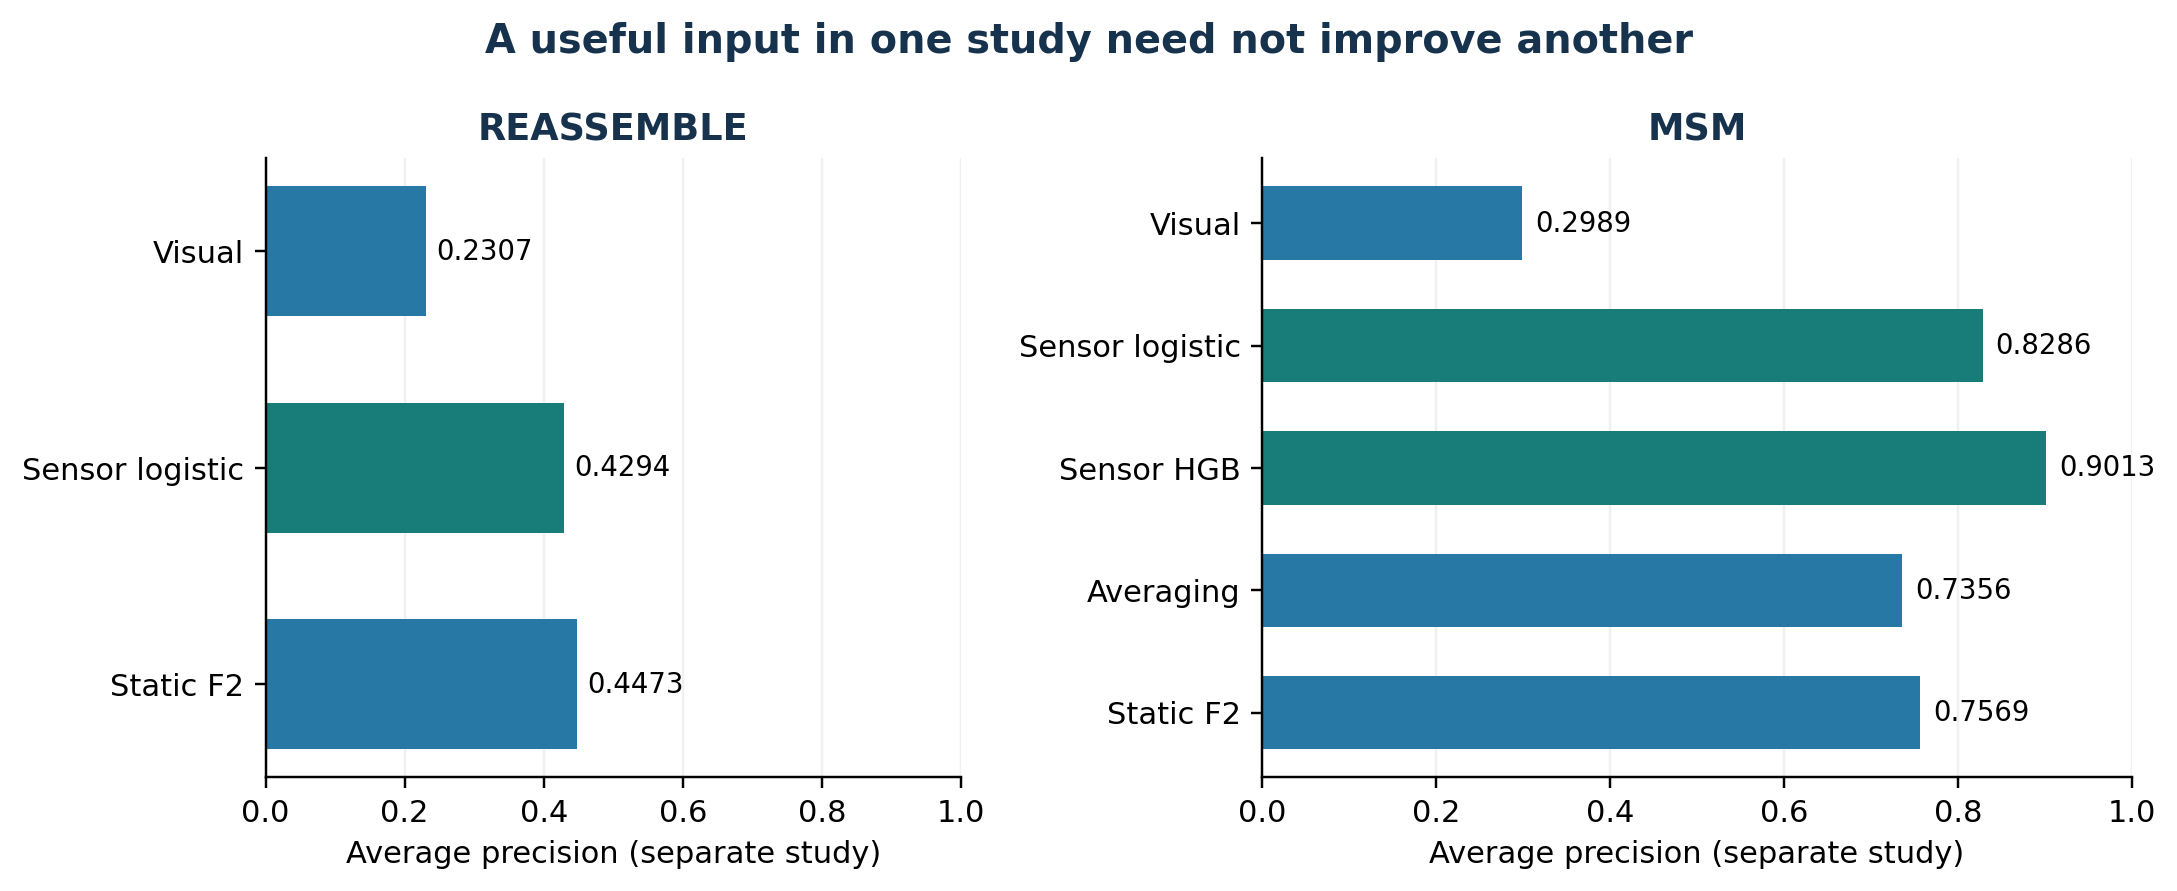
\includegraphics[width=\textwidth]{figures/within_study_results.png}
\displaynote{REASSEMBLE uses pooled failure average precision for 4,530 actions. MSM uses the mean of three seed-specific average precision scores, each calculated from pooled outer-fold predictions. The panels have different targets, prevalence, and evaluation protocols. The panel values and their sources are listed in Appendix~\ref{app:reproducibility}, \EvidenceRef{E107}{}.}
\end{figure}

\section{Robustness and Reliability --- Answer to SQ3}
SQ3 asks whether a gate improves robustness when inputs are missing, degraded, or unreliable. A known outage and a plausible but erroneous reading require different responses. PHM illustrates the distinction even within the sensor stream. In its separate four-arm diagnostic, one nominal group had no input columns, so dropping it removed no information. The gate was computed from context, so corrupting inputs to the other branches could leave its weights unchanged. Small changes around an already weak regression predictor give limited evidence about reliability. The photographs supplied the target in the principal comparison, leaving inference-time camera loss outside that experiment.\ev{PHM group dropout and conditioning}{\EvidenceRef{E004}{section 12.6}}

In REASSEMBLE, known complete loss of a stream routed the prediction to the surviving branch. Every fusion rule using that policy inherited the survivor's score. When both streams remained present and the sensor stream received Gaussian noise at one training standard deviation, stacking gave AP of .222 and the quality-only and combined gates gave .175 and .179, respectively. Intact vision alone achieved .231. Responding to noise by changing a weight therefore did not ensure a better failure ranking. The result pertains to this corruption and severity.

A later context-conditioned adjustment to the static REASSEMBLE stacker raised clean AP from .4473 to .4683. Its paired clean increment was .0210 (95\% CI [.0015, .0419]). Under matched augmentation, the mean adaptive increment over six corruption conditions was .0097 (95\% CI [$-.0034$, .0228]). A further pilot comparing a quality interaction with an exposure-matched static model also left its primary robustness increment unresolved, .0030 (95\% CI [$-.0267$, .0322]). These follow-ups support a gain for a particular adjustment on clean data. They do not show that conditioning on the measured quality variables improved decisions across degraded inputs.\ev{Distinct adaptive investigations}{\EvidenceRef{E004}{sections 18.2--18.3 and 19.5}}

In MSM, the strongest sensor noise reduced stacking to .207 AP. The augmentation-trained gate reached .299, approximately the score of intact vision alone. Under the strongest image blur, the same gate reached .683, below stacking at .771 and intact logistic sensing at .829. In HANDOVER, the strongest blur left averaging at .779 versus .824 for intact logistic sensing. Known complete loss used an explicit fallback. The participant grouping requirement prevented evaluation of a learned gate there (Appendix~\ref{app:handover}). ViFailback evaluated a clean camera-view ablation. The SQ3 corruption tests were outside its final computational budget, leaving the effect of degradation on its predictors unmeasured.

REASSEMBLE, MSM, and HANDOVER implemented a fallback to the surviving predictor when a stream was declared absent. Across the five studies, a consistent predictive gain from adaptive weighting under degraded but present inputs remains unresolved. A fair test gives the static and adaptive models the same corruption exposure and calibration opportunities, then compares each with the intact or degraded single stream available in that condition. Whether such a gate improves weld-quality decisions under sensing failures remains open.

\section{Evaluation Beyond Accuracy --- Answer to SQ4}
The PHM error measures agreement with image-derived candidate area in percentage points per run. For SQ4, interpreting that agreement as physical damage requires an independent measurement. Twenty nominal runs came from three gear experiments. Holding out a whole experiment tests whether the predictor generalizes beyond runs from experiments represented during fitting. Uncertainty estimated from saved run predictions remains conditional on the fitted models.

REASSEMBLE shows how to distinguish failure ranking, probability calibration, and the threshold at which an operator would act. The positive AP increment over sensors did not resolve every recall or calibration contrast. A review of 64 selected action clips found 57 agreements among 59 determinate judgments, with five indeterminate and two disagreements. The review exposed uncertainty about outcome visibility and boundaries. Its stratified sample and single reviewer limit population-level estimates of annotation accuracy (Appendix~\ref{app:human-review}). Recorded timings for the visual, sensor, and fusion components describe a warmed computation with prepared inputs. Operational latency also includes acquisition, completion of the observation window, and the response to a prediction.

At seed 42 in MSM, stacking had a lower Brier score than logistic sensing (.056 versus .062), even though logistic sensing ranked abnormal intervals better. In ViFailback, failure prevalence exceeded 85\%. At seed 42, stacking achieved failure AP of .945 and success AP of .312, yielding macro-AP of .629 (Table~\ref{tab:vif-bothclass}). Reporting both classes exposed a weakness that the majority-class score concealed. Task-cluster intervals characterize variation over the assessed tasks conditional on the fitted models. Session and operator dependence remain additional sources of uncertainty.

In HANDOVER, 110 of the 151 test trials were failures. At a threshold of .5, a training-prior predictor labelled every trial a failure, achieving failure F1 of .843 and zero specificity for successes. The official split remained usable for evaluating fixed baselines, while unavailable participant identifiers prevented participant-level uncertainty estimates for their contrasts. These examples support reporting prediction time, label provenance, class-specific discrimination, probability error, threshold consequences, and the grouping used for uncertainty. The branch predictions and fitted coefficients show how each stream contributed to a fused score. Establishing whether operators interpret it correctly or can act in time would require prospective observation and a usability study.

\section{Agreement and Disagreement With Previous Research}
Evidence from welding itself qualifies the expectation of a fusion advantage. In one penetration-state study, the clean image-only, audio-only, and fused models each reached 100\% accuracy \citep[Tables~1--3]{Hua2026Weld}. Distinct physical measurements may be available even when the reported endpoint leaves no measurable room for a clean gain. In the published HANDOVER study, five-class outcome accuracy averaged over five trainings was 69.1\% with video and force/torque and 67.9\% after gripper state was added \citep[Table~III]{Thoduka2024Handover}. The present HANDOVER implementation uses binary outcomes, different models, and failure AP. The common finding is that an additional stream can lower performance on a shared outcome. Absolute scores from the two experiments answer different questions.

Other industrial studies report clear gains within their respective protocols. Acoustic--thermal gearbox monitoring achieved 99.54\% mean accuracy against 90.54\% for the stronger individual thermal stream on a random within-condition split \citep[Table~2]{Ying2025Trustworthy}. On MVTec~3D-AD, combining RGB and 3D inputs raised mean image AUROC to 93.7\% from 88.0\% for RGB alone \citep[Table~3]{Rudolph2023Asymmetric}. These results concern different acquisition regimes and outcomes from completed-action failure. Conversely, studies of multimodal optimization and industrial input subsets identify losses against stronger individual channels \citep{Wang2020What,Horwitz2023Back,Goodarzi2023Deep}. REASSEMBLE and the external studies provide evidence in both directions. The performance differences alone cannot identify whether limited visibility, an unsuitable representation, or the fusion training procedure caused a particular loss.

Previous work provides both a theory and experimental tests of quality-aware weighting \citep{Zhang2023QMF}. RGB--geometry research tests absent 3D input \citep[Table~3]{P026}, and fuzzy-regularized camera--telemetry fusion tests corruption in simulated robot pose regression \citep{Altinses2023Fuzzy}. Training-time removal of images, a model designed for single-stream inference, an unannounced sensor malfunction, and adaptation with target-domain data impose different information constraints. The remaining question for a particular industrial task is whether a quality signal changes decisions beneficially once the static and unimodal controls have comparable observations, calibration, and training exposure.

\section{Lessons Across Datasets and Limits of Comparison}
Table~\ref{tab:cross-study} returns to the main research question. The units range from gear runs to individual actions, milling intervals, manipulation episodes, and handovers. Within each study, the single-input and fused models can be compared directly. Differences in targets, observation windows, class frequencies, and splits preclude a common ranking across datasets.

\begin{table}[htbp]
\caption{Interpretation of the Results Within Each Study}\label{tab:cross-study}
\centering\small

\begin{tabularx}{\textwidth}{P{27mm}YYY}
\toprule Study & Target/unit & Supported lesson & Principal boundary\\\midrule
PHM & Photo-derived proxy per gear run & Three sensor groups gave no clear improvement over the training mean & Physical damage reference unavailable\\
REASSEMBLE & Completed action failure & Stacking improved on sensors. Equal averaging performed similarly & Extra calibration step in stacking\\
MSM & Abnormal milling interval & Sensor models ranked abnormal intervals more accurately than stacking & Five dates in the paired interval\\
ViFailback & Whole-episode outcome & Original stacking fell below logistic sensing. Encoder transfer had mixed effects & Target-CNN adaptation and corruption tests deferred\\
HANDOVER & Success or failure of a handover trial & Averaging improved on vision alone but fell below logistic sensing & Participant grouping for learned fusion unresolved\\\bottomrule
\end{tabularx}
\displaynote{Each effect applies to the evaluation protocol for its study.}
\end{table}

MSM and HANDOVER reused a visual feature extractor and refitted predictors to their local targets. ViFailback additionally tested parameters learned on REASSEMBLE by fitting fresh heads on the transferred features. Reusing a procedure, transferring learned weights, and deploying an unchanged predictor on a new physical installation each require different evidence. Figure~\ref{fig:gap-coverage} locates the completed comparisons within the literature synthesis. The accompanying matrix identifies the studies and the comparisons underlying each question.
\begin{figure}[htbp]
\caption{Literature Comparisons and Experimental Coverage}\label{fig:gap-coverage}
\centering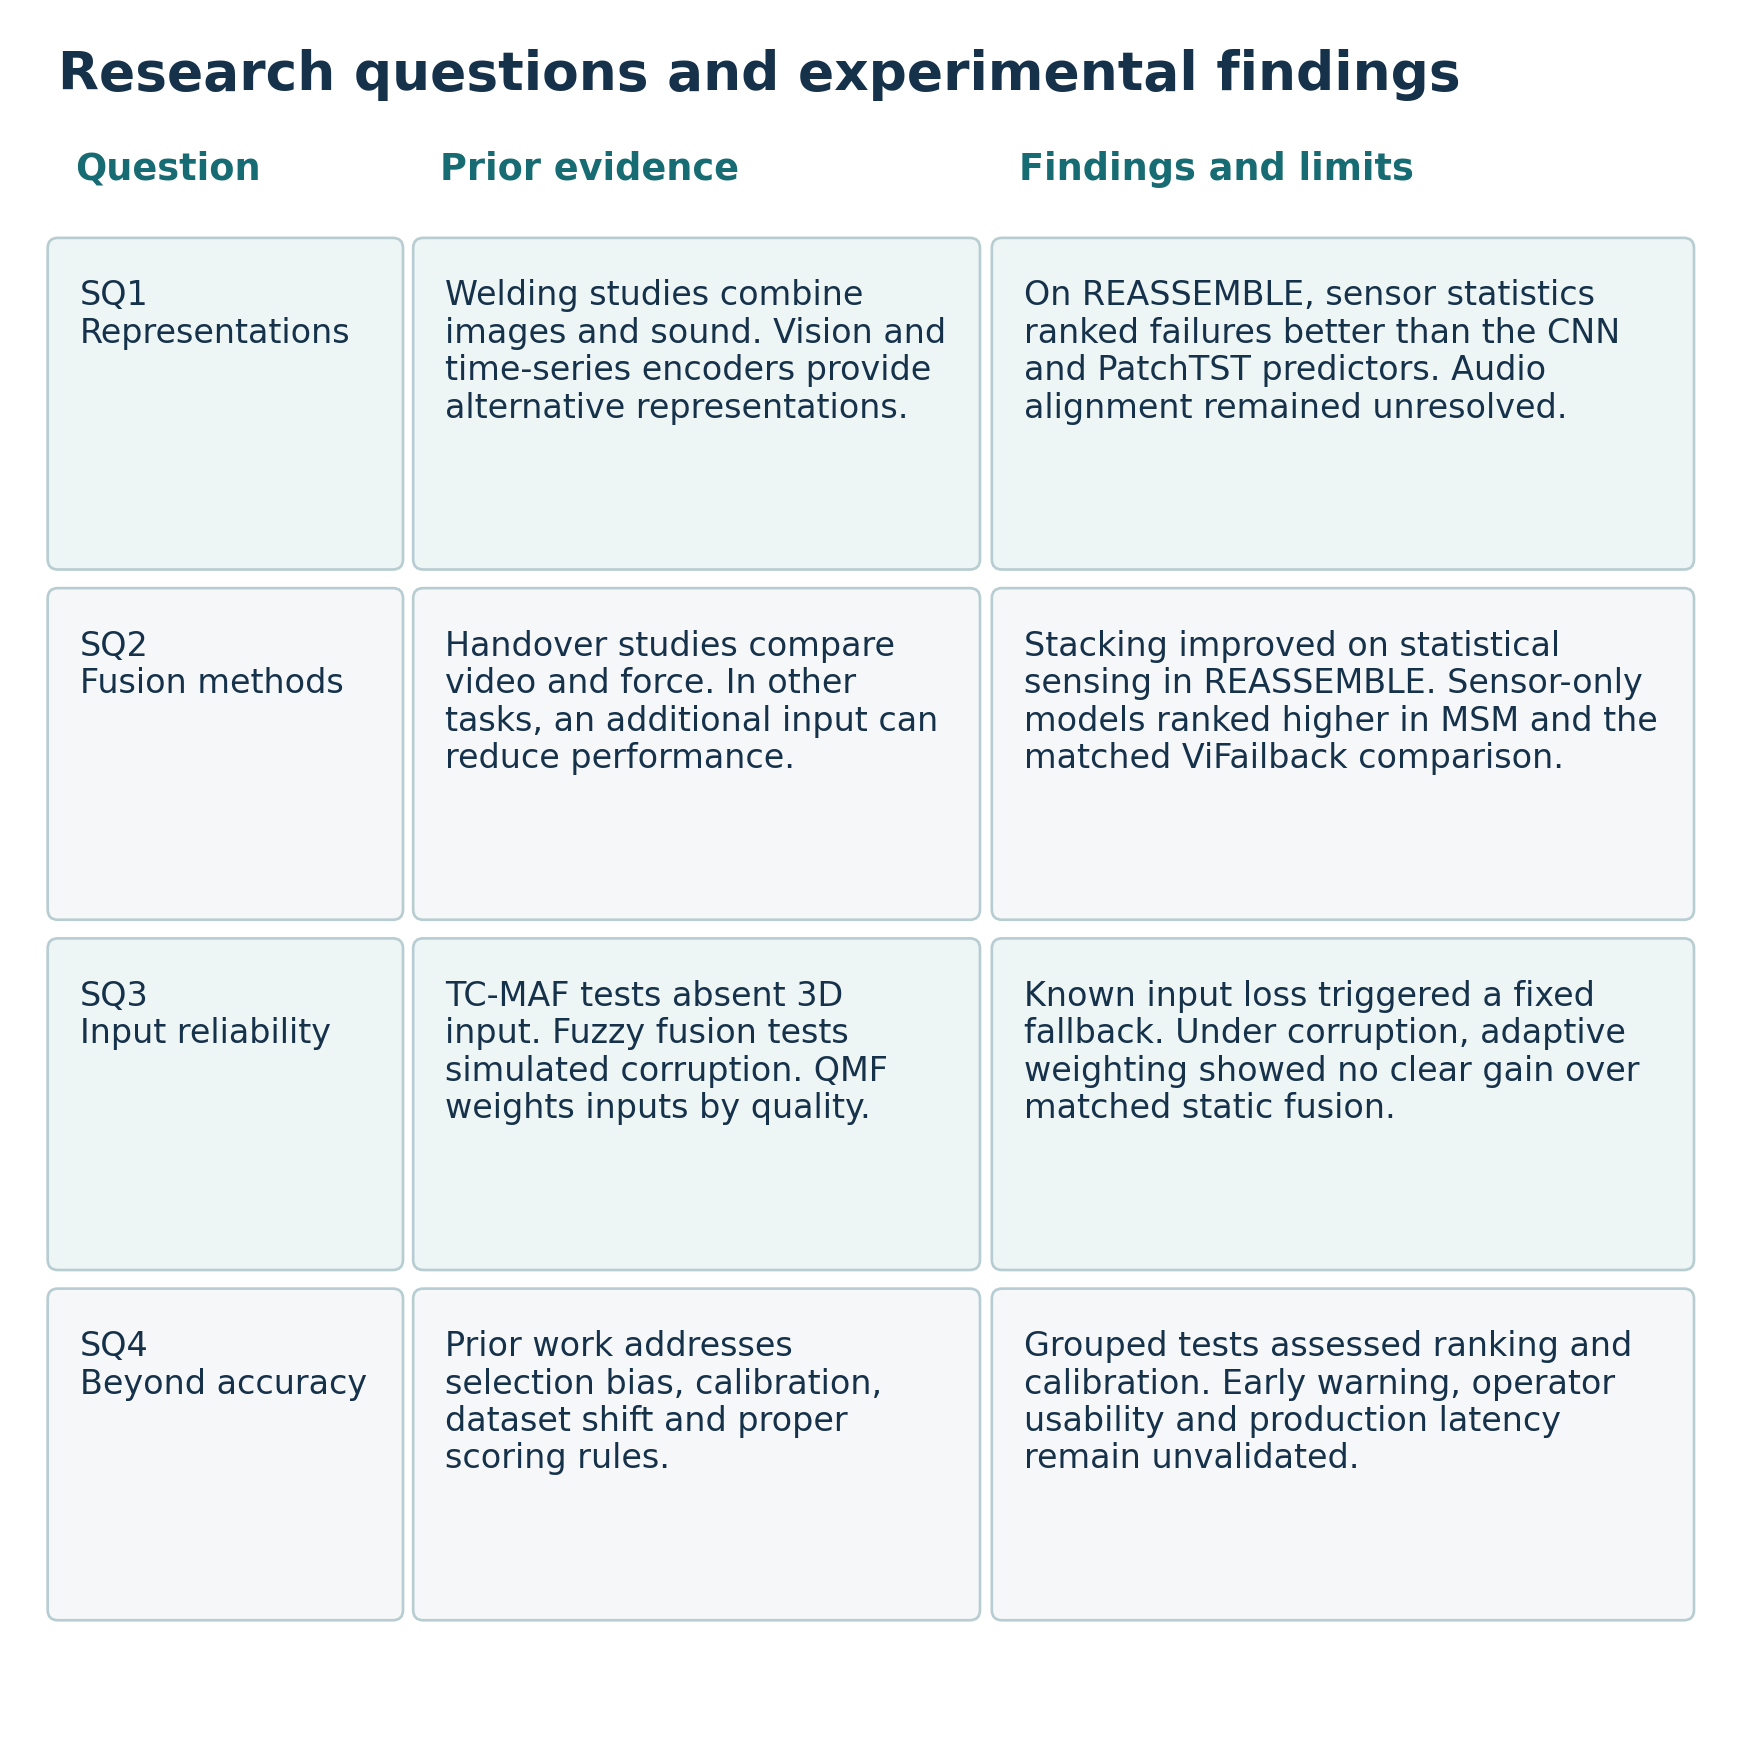
\includegraphics[width=\textwidth]{figures/gap_coverage.png}
\displaynote{The middle column summarizes prior research. The right column gives the corresponding experimental findings and limits.}
\end{figure}

\section{Threats to Validity and Unresolved Evidence}
Three features of the data limit a causal interpretation of architectural differences. First, the target may only approximate the phenomenon of interest. PHM has no independent quantitative tooth-damage reference, MSM's label mapping defines which intervals count as abnormal, and some robotic outcomes remained ambiguous under visual review. Second, the number of independently acquired units can be much smaller than the number of predictions. Gear experiments, recording sessions, dates, tasks, and participants capture different sources of dependence. Where identifiers were missing, independence across those groups could not be verified. Third, several later analyses revisited assessment populations examined during development. Intervals conditional on fitted predictions and variation over a few seeds do not capture that selection history.

Preprocessing before the separate four-arm PHM loop limits attribution of its results to architecture. In other experiments, differences in calibration, capacity, training budget or corruption exposure accompanied architectural changes. Some historical configurations lack the detail needed to reconstruct training exactly. ViFailback evaluated clean predictions from frozen visual backbones. Target-CNN adaptation and corruption effects were outside the final evaluation (Chapter~8). The literature synthesis covers the full texts available to a single reviewer.

Finally, the completed-window studies allowed the predictor to observe evidence near the outcome. Synthetic blur, noise, or stream removal test specified interventions. They give limited information about gradual calibration drift, unobserved timing faults, or shifts to another physical machine. Transferring a predictor to an earlier decision time or a different installation requires observations at that time and place.

\section{Implications for Multimodal System Design}
In a monitoring application, the intended decision determines what constitutes failure, how it can be confirmed independently, and which observations arrive in time to be useful. Evaluating each stream on the same held-out units establishes what it can predict alone. Equal averaging and a fitted static combination then provide references for testing whether context-dependent weights add value. When an instrument declares an outage, the remaining predictor supplies a natural reference. When faulty values still appear plausible, the relevant test is whether the gate recognizes situations in which trusting that stream would worsen the prediction.

A prospective return to welding could reserve whole welding sessions, collect an independent weld-quality measure, and fix the prediction horizon before examining those outcomes. On the same welds, exposure- and calibration-matched models could be assessed for clean performance, known absence, degraded readings, timing error, and shifts between operating conditions. Paired effects and a prespecified tolerance for clean-performance loss would clarify the operational cost of any robustness gain. Such a test would show whether the modest gain for completed assembly actions carries over to weld-quality decisions.

\chapter{Conclusion and Future Work}
\label{ch:conclusion}

\section{Answer to the Main Research Question}
The study began with two questions about weld quality. Could a camera reveal changes that machine signals missed? Would the combined prediction remain reliable if either input deteriorated? The architecture comparison extended to gear monitoring and robotic assembly. By the time the Intel Welding data were re-examined, development had already drawn on the proposed test recordings. Independent welding validation would require a new set of welds. The five studies evaluated related questions against the outcomes available in each dataset (Appendix~\ref{app:chronology}).

In PHM, post-run photographs supplied a continuous measure of candidate damage area on gear teeth. The photographs defined the target for sensor regression. Across held-out experiments, combining three sensor groups gave a mean absolute error of 0.824 percentage points, compared with 0.804 for predicting the training mean (Table~\ref{tab:phm-loeo}). The paired interval allowed either model to have lower error. Even an accurate prediction of this proxy would still require independent measurements to establish how closely the photographed area tracked physical damage.

REASSEMBLE made a direct fusion comparison possible. Video and machine signals covered the same completed action, each action had a recorded outcome, and entire recordings could be held out for assessment. Across 4,530 actions from 148 recordings, logistic stacking achieved failure average precision (AP) of .447, compared with .429 for its sensor component and .446 for equal probability averaging (Tables~\ref{tab:reassemble-unimodal} and~\ref{tab:reassemble-fusion}). The recording-level bootstrap supported a gain over sensors for these fitted models. The difference between stacking and averaging remained uncertain. Because the sensor predictor lacked a matched second calibration stage, the comparison cannot isolate how much of the gain came from the visual input itself.

The external studies tested whether the same finding held for different targets. In MSM, stacking ranked abnormal milling intervals less accurately than the logistic sensor model, with average precision across seeds of .757 and .829, respectively (Table~\ref{tab:msm-clean}). In ViFailback, the target was the outcome of a whole manipulation episode. Across three seeds, stacking yielded macro-AP of .621--.629 against .649 for logistic sensing. Initializing the visual encoder from REASSEMBLE gave mixed results across the matched runs (Tables~\ref{tab:vif-bothclass} and~\ref{tab:vif-matched}). In HANDOVER, averaging video and force--torque predictions on 151 trials yielded mean failure AP of .803, below the sensor component at .824 (Table~\ref{tab:handover-clean}). Participant-to-trial identifiers were unavailable, so the supplementary study could not construct the participant-disjoint predictions needed to train and evaluate its proposed stacker.

Taken together, the studies support a modular architecture in which each observation can be evaluated on its own before its predictions are combined with another stream. The value of that combination depended on the target, the available observations, and the strength of the sensor predictor. The results concern gear-condition estimation and retrospective classification of completed operations. Independent weld-quality detection remains the unanswered application of the original question.

\section{Supported Contributions}
The representation comparison (SQ1) favored sensor statistics on the main assembly task. In REASSEMBLE, the frozen ResNet18-vd backbone inside the pretrained RT-DETR-R18vd checkpoint supplied pooled frame features to a binary action classifier. Engineered sensor statistics outperformed the short-budget PatchTST time-series Transformer in the principal assembly comparison. Pooling features near the action boundary improved a separate exploratory visual result. The suitability of pretrained audio representations remains open because audio alignment did not support a predictive comparison.

For fusion choice (SQ2), the shared assembly cohort allowed feature concatenation, probability averaging, logistic stacking, and scalar gates conditioned on process context to be evaluated on the same actions. Feature concatenation reached AP of .412. The simpler prediction-level combinations ranked failures more accurately under the tested training procedures. The external results qualify that finding by identifying tasks on which even the learned combination fell below its sensor component.

For missing or degraded inputs (SQ3), a known missing stream could be handled by routing predictions to the available model. When a stream remained present but became unreliable, the two original gates evaluated under corruption showed no consistent advantage. Under strong sensor noise in REASSEMBLE, stacking fell to AP .222, below the intact visual predictor at .231. A subsequent gate that adjusted a static prediction using context improved clean performance in an exploratory comparison. Tests with matched corruption exposure left its robustness gain unresolved. This gate and the later visual pooling method were evaluated in separate experiments.

For evaluation beyond accuracy (SQ4), the distinction between ranking failures and estimating their probability affected model choice. On the seed-42 MSM comparison, stacking yielded a lower Brier score than logistic sensing (.056 and .062, respectively), although sensing ranked abnormal intervals more accurately. Grouped analyses, uncertainty estimates, a review of action labels, and component timings exposed different limits on reliability and practical use. The code and configuration records identify which branches and fusion rules produced these results. The literature matrix places them alongside prior welding, camera--sensor, and missing-input studies and narrows the open question to the performance of adaptive weighting under comparable training and calibration conditions.

\section{Principal Limitations}
Each dataset imposes a different evidential limit. PHM lacks an independent physical reference, and the preprocessing order in its separate four-arm diagnostic prevents a leakage-free interpretation of that experiment. The industrial and robotic datasets offer incomplete information about independence at the level of tools, objects, or participants. Complete-action and complete-episode predictions can use evidence that only becomes visible near the outcome. Deploying a warning system would require a prediction horizon that excludes such information.

The comparison also depends on how the models were fitted. Calibration, training budgets, and exposure to corruptions differed in some comparisons. Several follow-ups revisited previously evaluated populations, and the reported bootstrap intervals condition on the fitted models. The short-budget fine-tuning comparison did not resolve a mechanism for the observed differences. Some longer training runs and planned sensor-degradation evaluations remained incomplete. Where only run summaries were available, they limited the scope for independent checks of individual predictions.

\section{Priorities for Future Research}
An independent welding study is the most direct next test of the original question. It should specify the weld-level outcome and prediction time, pair the camera and process measurements to that decision, and reserve complete new welding sessions for assessment. An independent inspection should establish weld quality. For PHM, a physical measure of damage linked to a known tooth would likewise distinguish measurement validity from the ability to predict the photographic proxy. Independent review of ambiguous robotic outcomes would strengthen the corresponding classification targets.

Within each study, the informative comparison is between the strongest single-input predictor, equal averaging, a fitted static combination, and a gate trained with comparable calibration opportunities and corruption exposure. Repeated tests of known absence, unannounced corruption, temporal misalignment, and shifts between physical groups would show which failure conditions justify adaptive weighting. Prespecified margins for clean performance and grouped uncertainty estimates would make the cost of a robustness improvement visible.

The remaining transfer experiments require matched optimization budgets, normalization procedures, and held-out tasks. For operational monitoring, prospective tests should also measure warning time, false alarms, and end-to-end delay, and evaluate how operators act on uncertain predictions. These measurements would establish whether the modest ranking benefit observed on completed assembly actions translates into a useful decision while a weld is still in progress.

\ifdefined\ThesisReviewCopy\else
\clearpage
% Use the top text margin for this standalone disclosure. The four paragraphs
% retain the manuscript's regular type size, margins and double spacing.
\begingroup
\makeatletter
\renewcommand{\@makeschapterhead}[1]{%
  {\parindent=0pt\raggedright\normalfont\Huge\bfseries #1\par}%
  \nobreak\vspace{6pt}}
\makeatother
\chapter*{AI Assistance Disclosure}
\addcontentsline{toc}{chapter}{AI Assistance Disclosure}
\endgroup
\noindent
The author defined the scope of the research, provided the implementation records and saved experimental results, obtained full-text publications, and reviewed how the methods and findings were interpreted and presented. Preparation of the manuscript involved AI-assisted drafting and revision. The author used AI tools to develop and refine the text, including the abstract, and to examine whether descriptions of the models, experiments, and results were consistent with the available evidence.

The author conducted the literature research and critically reviewed the papers, assessing how their methods, choice of baselines, and evaluation conditions supported their findings. AI tools helped the author prioritise papers for closer reading, locate relevant passages and tables during review, and organise the evidence into a comparison matrix. During the November revision, the author obtained additional publications and used AI assistance to match their titles and DOIs to Zotero records and check the corresponding PDF attachments. AI tools also supported numerical consistency checks, bibliography processing, APA citation editing, figure preparation, LaTeX editing and compilation, and the extraction of chapter text.

The manuscript revision drew on existing publications, implementation records, and saved experimental outputs, without new model training or inference on raw data. The thesis distinguishes findings reported in publications, checks documented in earlier experiment records, and checks performed on saved outputs during revision. AI-assisted appraisal formed part of the same review process and provided no independent second human assessment. Ambiguous source claims, incomplete experiments, and unresolved questions of physical validation are documented as limitations.

Appendix~\ref{app:prompt-record} presents two reconstructed examples of implementation and audit requests. Section~\ref{sec:results-archiving} summarises AI assistance in planning local archiving and Git version control for experimental outputs. OpenAI Codex assisted with the implementation and audit tasks and with preparation of Figure~\ref{fig:fusion-interfaces} \citep{OpenAICodex}. The records do not identify the model version used in earlier implementation sessions.

\clearpage
\printbibliography[heading=bibintoc,title={References}]
\appendix
\chapter{Literature Search Records and Evidence Tables}
\label{app:literature}
\section{Discovery Population and Evidence Status}
The screening record dated 16 November 2026 lists 120 unique candidates. Of these, 39 met the inclusion criteria, 37 were excluded and 44 remained potentially relevant but insufficiently verified. The corresponding full-text appraisal covered 37 of the 39 included works. The two accessible only through abstracts and bibliographic metadata contributed to the screening counts but supplied no methodological or numerical findings.\ev{Historical search and screening record}{\EvidenceRef{E006}{}, \EvidenceRef{E009}{}, \EvidenceRef{E005}{}}

The subsequent appraisal covered 59 PDF files. Two pairs were byte-identical, leaving \ExpandedPDFCount{} distinct files. Titles, authors, DOIs and repository identifiers showed that these represented \ExpandedPDFCount{} additional works, bringing the total appraised to \ReviewWorkCount{}. This total includes empirical industrial studies, transferable methods, statistical and representation methods, dataset descriptions and contextual studies.

The search log for this screening round records more than 15 distinct queries. Several queries returned results together, precluding an exact count of the records retrieved by each. The subsequent appraisal drew on additional accessible full texts and used publisher or repository pages to check bibliographic identities and versions. This procedure limits the review's coverage to the works identified and accessible through these routes.\ev{Expanded appraisal and counts}{\EvidenceRef{E016}{}, \EvidenceRef{E010}{}, \EvidenceRef{E011}{}, \EvidenceRef{E012}{}}

\section{Extraction, Locators, and Versions}
For each study, the appraisal recorded the prediction unit and target, physical inputs, derived representations, fusion method, single-input comparisons and assignment of data to training and evaluation. Missing inputs, noisy inputs and changes of operating conditions were coded separately. Numerical findings cite the relevant page, table or figure. Where the available text left a procedure unspecified, its status was recorded as unknown.

The appraisal distinguishes the published bibliographic record from the version examined. Preprints and journal articles sometimes give different sample counts for the same work. File hashes identify the version used for each extraction. The 37 initial full-text records include 148 short quotations that locate the evidence for their codes. The review compared reported methods and results without rerunning the published experiments.\ev{Extraction and identity records}{\EvidenceRef{E007}{}, \EvidenceRef{E008}{}, \EvidenceRef{E017}{}, \EvidenceRef{E014}{}}

\section{Comparison Matrix and Denominators}
Table~\ref{tab:literature-matrix} gives the codes for the initial 37 studies. Table~\ref{tab:expanded-register} identifies the contribution and principal limitation of each of the 57 additional works. The accompanying matrix gives the missing-input, noise and shift tests for individual studies, together with source locations.\ev{Full expanded comparison register}{\EvidenceRef{E013}{}, \EvidenceRef{E015}{}}

Within-protocol input variants do not guarantee equal capacity, pretraining, calibration or selection budget. Planned single-input deployment, missing training images, generated substitution, stochastic dropout and unexpected inference outage are different conditions. Ordinary defective objects, natural geometric gaps and fixed noisy data are not automatically controlled corruption experiments. The codes describe this inspected evidence and cannot estimate field-wide prevalence.

\begin{longtable}{@{}p{0.33\textwidth}llllll@{}}
\caption{Comparison of the 37 Original Full-Text Studies}\label{tab:literature-matrix}\\
\toprule Study & Data & Fusion & Base & Missing & Noise & Shift \\
\midrule\endfirsthead
\toprule Study & Data & Fusion & Base & Missing & Noise & Shift \\
\midrule\endhead
\citep{Wang2025A} & VIB & H & U & N & S & A \\
\citep{Ying2025Trustworthy} & CAM-S & H & M & N & S & N \\
\citep{Huang2026Rolling} & AUD-VIB & I & M & N & S & C \\
\citep{Gu2024Improved} & AUD-VIB & I & P & N & N & N \\
\citep{Yang2024Fault} & MS & I & M & PA & N & N \\
\citep{Ma2025A} & IMG-U & I & M & TR & N & N \\
\citep{Li2025PGMTKD} & MS & KD & R & PA & N & N \\
\citep{AlDulaimi2019A} & SV & I & L & N & S & N \\
\citep{Li2025MADFlow} & RGB-G & I & A & N & N & N \\
\citep{Wan2024Pipeline} & AUD & E & M & N & N & N \\
\citep{Baltrusaitis2019Multimodal} & X & TAX & S & NA & NA & NA \\
\citep{Sui2026Incomplete} & RGB-G & KD+L & M & PA & N & N \\
\citep{Cheng2025Multimodal} & RGB-G & H & M & N & N & N \\
\citep{Xu2025ModalityResilient} & RGB-G & KD+H & P & SD & N & N \\
\citep{Shangguan2025CPIR} & RGB-G & H & A & N & N & N \\
\citep{Altinses2025Performance} & SIM-CS & I & A & GS & N & T \\
\citep{Wang2023Multimodal} & RGB-G & H & M & N & N & N \\
\citep{Horwitz2023Back} & RGB-G & E & M & N & N & N \\
\citep{Costanzino2024Multimodal} & RGB-G & H & A & N & N & N \\
\citep{Rudolph2023Asymmetric} & RGB-G & I & M & N & N & N \\
\citep{Bonfiglioli2023The} & SIM-G & E & M & N & N & N \\
\citep{Bergmann2022The} & RGB-G & E & P & N & N & N \\
\citep{Wang2020What} & X & I & M & N & N & N \\
\citep{Xie2025Audiovisual} & CAM-S & I+KD & M & PA & S & N \\
\citep{Goodarzi2023Deep} & MS & E+I & M & N & S & N \\
\citep{Roth2022Towards} & RGB & U & U & N & N & N \\
\citep{Bergmann2019MVTec} & RGB & U & U & N & N & N \\
\citep{Purohit2019MIMII} & AUD & U & U & N & B & N \\
\citep{Koizumi2019ToyADMOS} & AUD & U & U & N & B & N \\
\citep{Koizumi2020Description} & AUD & U & U & N & F & N \\
\citep{Chu2024A} & AUD-VIB & I & N & N & N & A \\
\citep{Kullu2022A} & MS & I & M & N & N & N \\
\citep{Chen2023Multisensor} & CAM-S & E & M & N & N & N \\
\citep{Li2022A} & OPT-AUD & I & M & N & N & N \\
\citep{Petrich2021Multimodal} & CAM-S & I & M & RS & N & N \\
\citep{Pandiyan2022Deep} & OPT-AUD & E & N & N & N & W \\
\citep{Bevans2023Heterogeneous} & MULTI-CAM & E & A & N & N & B \\
\bottomrule
\end{longtable}
\displaynote{All 37 records have evidence status F. The codes describe the inspected protocol. They do not rate study quality.}
\noindent\textit{Data:} CAM-S denotes a physical camera and a separate non-image signal; RGB-G denotes RGB and geometry; OPT-AUD denotes photodiode and acoustic signals, without a camera input. MS denotes machine/process channels; SV denotes parallel representations of the same telemetry; IMG-U has incompletely documented image provenance. SIM-CS/SIM-G are synthetic. RGB, AUD and VIB are single physical modalities; MULTI-CAM uses several imaging sources; X is transferable non-industrial evidence.
\par\noindent\textit{Fusion:} E, early; I, intermediate; L, output-score fusion; H, hybrid feature/output fusion; KD, privileged cross-modal training; U, unimodal; TAX, taxonomy. Authors' terminology is normalized by where information is combined.
\par\noindent\textit{Baseline:} M, input variants evaluated within one protocol; P, partial/ambiguous; R, retained-input student with/without teachers; L, literature comparison; A, module/map/task ablations only; U, unimodal reference; S, survey; N, not established. M does not guarantee matched capacity, pretraining or tuning.
\par\noindent\textit{Missing:} PA, planned missing-input inference; SD, simulated dropout; TR, missing training images with complete tests; GS, generated substitution; RS, retrained input subsets; N, no controlled trial established; NA, survey. \textit{Noise:} S, synthetic intervention; B, recorded-background mixing; F, fixed noisy benchmark; N, no controlled trial established. \textit{Shift:} A, target-adaptive transfer; C, condition transfer with target validation; B, independent-build/layout transfer with limited outcome coverage; T, simulated translation; W, unseen window duration; N, no held-out domain transfer established.


\begingroup\small
\begin{longtable}{@{}P{.25\textwidth}P{.16\textwidth}P{.53\textwidth}@{}}
\caption{Full-Text Appraisal of the 57 Additional Works}\label{tab:expanded-register}\\
\toprule Work & Evidence role & Appraisal focus and qualification \\
\midrule\endfirsthead
\toprule Work & Evidence role & Appraisal focus and qualification \\
\midrule\endhead
P001 \citep{P001} & Context & Single infrared image restoration; no independently acquired second modality. This is context rather than evidence for a fusion advantage. \\
P002 \citep{P002} & Context & Infrared machinery diagnosis. Combining thermal regions remains image-only; vibration fusion is proposed as future work. \\
P003 \citep{P003} & Industrial & Physical camera and audio welding classification. Split independence and controlled missing/noise evaluation are not established in the inspected postprint. \\
P004 \citep{P004} & Methods & Seminal evaluation foundation on model-selection bias. It does not supply an industrial fusion experiment. \\
P005 \citep{P005} & Methods & Transferable modality-dropout method. Training exposure and planned available-input configurations determine the robustness claim. \\
P006 \citep{P006} & Methods & Transferable gated intermediate fusion. Learned allocation alone does not establish calibrated modality reliability. \\
P007 \citep{P007} & Methods & Transferable robust multimodal classification architecture. The inspected preprint and published journal metadata refer to one work. \\
P008 \citep{P008} & Methods & Predictive uncertainty under dataset shift. Good in-distribution confidence does not guarantee shifted reliability. \\
P009 \citep{P009} & Methods & Reproducibility and reporting foundation. Documentation and code availability are distinct from independently reproduced results. \\
P010 \citep{P010} & Methods & The visual patch Transformer was evaluated on image recognition. The study provides no comparison of the industrial visual models evaluated here. \\
P011 \citep{P011} & Methods & The audio-spectrogram Transformer represents sound through spectrogram patches. The present studies include no completed audio-branch comparison. \\
P012 \citep{P012} & Methods & Self-supervised dilated-convolution time-series encoder. It is not a Transformer; the reported Transformer substitution performs worse. \\
P013 \citep{P013} & Methods & The video Transformer models interactions across space and time. The REASSEMBLE visual classifier averages frame descriptors over time. \\
P014 \citep{Nagrani2021MBT} & Methods & Audiovisual attention-bottleneck fusion. Transferable representation design does not establish industrial sensor-failure robustness. \\
P015 \citep{P015} & Methods & Multimodal benchmark and evaluation framework. Its different tasks are not independent replications of one industrial target. \\
P016 \citep{P016} & Methods & The missing-modality Transformer evaluation includes adverse multimodal results. For the Food dataset, the prose and tabulated unimodal result disagree. \\
P017 \citep{P017} & Methods & The preprint and published article on leakage in scientific evaluation give different counts of affected papers. \\
P018 \citep{P018} & Methods & The study evaluates pretrained time-series representations on benchmarks. Transfer of its weights to the industrial tasks considered here was not tested. \\
P019 \citep{Sliwowski2025REASSEMBLE} & Dataset & The robotic assembly dataset provides native action outcomes. Its published demonstration count differs from the eligible sample for the present action-level analysis. \\
P020 \citep{P020} & Methods & Transferable multimodal negative-learning study. Its noise regimes and negative comparisons remain specific to the reported tasks. \\
P021 \citep{P021} & Industrial & Physical tool images and force measurements with adaptive fusion. Post-pass image timing and incompletely reported splits limit prognostic claims. \\
P022 \citep{P022} & Methods & Non-industrial dynamic-fusion method. Its evidence informs fusion assumptions without constituting industrial deployment validation. \\
P023 \citep{P023} & Methods & Transferable constrained fusion of text with time series. It supplies negative evidence against assuming every additional modality helps. \\
P024 \citep{P024} & Industrial & Industrial inspection using geometric prior information. RGB and geometry are distinguished from independent machine telemetry. \\
P025 \citep{P025} & Industrial & The industrial inspection model combines visual and geometric features with language for defect reporting. Its evaluation includes task-specific supervision and measures report consistency. \\
P026 \citep{P026} & Industrial & Train-calibrated RGB/geometry fusion includes explicit missing-3D evaluation and static/gated controls. It is not camera-plus-machine-telemetry evidence. \\
P027 \citep{P027} & Industrial & Audio, vibration and current fusion with missing-input claims. Limited auditability excludes it from strong quantitative synthesis. \\
P028 \citep{Thoduka2024Handover} & Dataset & Completed robotic handover outcomes with video, force/torque and gripper inputs. Added gripper input reduces one five-class accuracy result. \\
P029 \citep{Huo2022Multisensor} & Industrial & Thermal-image and vibration fault diagnosis with single-input and noise controls. Reliability conclusions remain conditional on its protocol. \\
P030 \citep{Nie2023PatchTST} & Methods & PatchTST was evaluated for time-series forecasting. The PHM regression and REASSEMBLE classification experiments trained separate temporal models from scratch. \\
P031 \citep{P031} & Industrial & Vision-language surface localization is evaluated with pixel metrics. These measure localization rather than image-level detection or numerical process sensing. \\
P032 \citep{Hua2026Weld} & Industrial & Camera/audio weld-penetration attention fusion. Clean single-input and fused models all report 100\% accuracy; independent-run splitting is unclear. \\
P033 \citep{P033} & Industrial & RGB/geometry disagreement scoring. Eyecandies image AUROC decreases despite improved localization, showing metric-specific trade-offs. \\
P034 \citep{P034} & Methods & Space-time attention models cross-frame interactions. The core REASSEMBLE visual representation averages frame descriptors. \\
P035 \citep{P035} & Context & Weakly supervised single-camera surface inspection. Internal feature fusion is not fusion of independently acquired physical modalities. \\
P036 \citep{P036} & Methods & Transferable counterargument on attention interpretation. Model inspection does not by itself establish a physical causal explanation. \\
P037 \citep{Altinses2023Fuzzy} & Simulation & Camera/robot telemetry corruption in simulated pose regression. Overlapping temporal windows and random splitting limit physical-deployment inference. \\
P038 \citep{P038} & Industrial & RGB/geometry consistency fusion. Its learned scalar mixing coefficient does not demonstrate sample-conditioned online reliability adaptation. \\
P040 \citep{Bengio2004CVVariance} & Methods & Cross-validation variance theory. Overlapping training folds do not supply independent replications for a naive standard error. \\
P041 \citep{Guo2017Calibration} & Methods & Validation-fitted calibration foundation. In-distribution temperature scaling is not a guarantee of reliable probabilities after shift. \\
P042 \citep{P042} & Context & Single-vibration diagnosis with synthetic noise. Simulated target training and reporting inconsistencies limit transfer and field-validity claims. \\
P043 \citep{P043} & Methods & Distribution-shift benchmark. OOD validation access is explicit; this is not an untouched-target industrial multimodal experiment. \\
P044 \citep{P044} & Methods & Transferable medical fusion counterexample. Selection and evaluation share validation data; no independent final test is established. \\
P045 \citep{P045} & Industrial & Post-pass tool photographs and acoustic emission predict wear. Strong visual and adverse multimodal comparators coexist with unresolved tool-split coverage. \\
P046 \citep{P046} & Industrial & Microphone/accelerometer bearing fusion. Test-noise results lack an equivalent static corruption comparator; recording-disjoint splitting is unclear. \\
P048 \citep{P048} & Industrial & Thermal-camera and vibration feature fusion. Overlapping windows, multirate pairing and separately fitted speeds restrict generalization claims. \\
P049 \citep{P049} & Methods & Transferable attention-interpretability critique. Attention perturbation is distinct from physical input corruption or modality dropout. \\
P050 \citep{P050} & Methods & Transferable unaligned language/audio/video cross-attention. Unequal feature rates are not a controlled hardware-clock offset test. \\
P051 \citep{P051} & Industrial & Visible/infrared federated detection. Incomplete clients differ from surprise inference outage; group splits, clipped results and coefficient conflicts limit appraisal. \\
P052 \citep{Kim2026MSM} & Dataset & Milling dataset with laboratory video and machine measurements. Dataset availability enables research but is not itself a learned fusion result. \\
P053 \citep{P053} & Industrial & Audio/vibration wavelet-image cross-attention. These are transformed signals, not camera images; controlled missing/noise tests are not established. \\
P054 \citep{P054} & Industrial & RGB/surface-normal anomaly detection. Training feature-noise regularization is distinct from a test-input degradation benchmark. \\
P055 \citep{P055} & Methods & Proper-scoring-rule foundation. Expected propriety does not certify finite-sample calibration or shifted sensor reliability. \\
P056 \citep{P056} & Industrial & RGB/point-cloud local alignment preprint, version 1. Checkpoint-selection population and retraining variability remain unclear. \\
P057 \citep{Zeng2026ViFailback} & Dataset & The study uses visual symbols and language to diagnose manipulation failures. The present ViFailback experiment instead combines camera views and numerical robot observations. \\
P058 \citep{Zhang2023QMF} & Methods & Transferable quality-aware weighting. Its conditional generalization-upper-bound comparison does not imply universal actual-risk superiority. \\
P059 \citep{Zhao2024RTDETR} & Methods & Single-image object detector foundation. Executing an extracted CNN backbone does not execute the full detector or its reported inference pipeline. \\
\bottomrule\end{longtable}
\displaynote{The accompanying CSV identifies each target, fusion method, control, test of missing, noisy, or shifted inputs, result, and source location. The role column distinguishes direct experimental evidence from background material.}\endgroup
\noindent\textit{Interpretation:} Transferable methods are non-industrial unless their record identifies a direct application. Dataset papers and unimodal/context references do not supply a multimodal fusion experiment. A retained preprint remains provisional. All source versions, complete qualifications and numerical locators are in the expanded register.


\section{Benchmark Identity and Assessment Populations}
The MVTec 3D-AD dataset paper lists 249 anomaly-free and 948 anomalous test samples, a total of 1,197. It reports 2,656 training and 294 validation samples separately \citep[Table~1, PDF p.~4]{Bergmann2022The}. UCF reports the same test count \citep{Cheng2025Multimodal}, whereas some other method descriptions give 1,137. The discrepancy leaves the samples underlying those comparisons uncertain. The review uses the published scores, whose comparability also depends on preprocessing, masks and metric definitions.

\chapter{Dataset Inventories, Exclusions, and Target Definitions}
\label{app:datasets}

\section{Registry Conventions}

Table~\ref{tab:dataset-registry} distinguishes the number of observations in each published release from the number eligible for a particular experiment. Eligibility depended on the target, the required inputs and the temporal correspondence between them. The counts refer to the dataset versions used in the reported experiments.

\small
\begin{longtable}{@{}P{.17\textwidth}P{.25\textwidth}P{.25\textwidth}P{.23\textwidth}@{}}
\caption{Prediction Targets, Units, and Eligible Populations}\label{tab:dataset-registry}\\
\toprule Dataset & Target and unit & Admitted population & Qualification \\
\midrule\endfirsthead
\toprule Dataset & Target and unit & Admitted population & Qualification \\
\midrule\endhead
PHM & Provisional image-derived candidate-area regression; tooth/run values and aggregated run target & v3: 20 run records, 24 teeth per run, 480 tooth/run values across EXP-A/B/F & Image reference is privileged/offline; only three experiment groups support the retained LOEO setting \\
REASSEMBLE & Completed high-level action failure; failure positive & 4530 actions, 509 failures, 148 recordings & Hand camera plus five sensor streams; 149 recordings in raw inventory \\
MSM & Native label 1 versus labels 0/2; cutting interval & 1895 intervals: 336 positive, 1559 negative & 2512 native intervals; 617 technical exclusions; 45 nominal experiment groups \\
ViFailback & Native whole-episode outcome, with failure positive & 4,382 episodes across 99 tasks (3,753 failures and 629 successes) & 5,202 native episodes, with 820 excluded or quarantined after reconciliation \\
HANDOVER & Handover failure; failure positive & 587 eligible trials: 335 train, 101 validation, 151 test & 589 native trials; two training exclusions; test 110 failure/41 success \\
Intel welding & Original industrial-monitoring setting & No independent weld-quality fusion evaluation & Feasibility-gate exclusion; not a trained-model performance result \\
\bottomrule
\end{longtable}


\section{Target Lineage and Pairing}

The PHM target \nolinkurl{phm2026_image_damage_v3} uses one deterministically selected view for each of teeth 5--28 and aggregates the three highest tooth values for each run. This gives a provisional image-derived proxy for physical deterioration. Earlier targets used different image geometry, view aggregation and tooth sets, which limits comparison of their errors. Sorting tooth values removes positional identity, so the profile describes their distribution within a run. The fixed image split and the leave-one-experiment-out sensor evaluation assess different populations.\ev{PHM target lineage and model mapping}{\EvidenceRef{E023}{}, \EvidenceRef{E110}{}}

The REASSEMBLE release reports 4,551 demonstrations. The analysis included 4,530 completed pick, insert, remove and place actions after applying the primary-action and input-completeness criteria. Of these, 509 were failures. Each action supplied 22 scalar sensor channels and a descriptor from 16 hand-camera frames. The core experiment excluded audio because the correspondence between annotation times and waveform times could not be independently established.\ev{REASSEMBLE cohort and gates}{\EvidenceRef{E044}{}, \EvidenceRef{E041}{}}

\section{External Cohorts and Exclusions}

MSM's primary target is intervention-worthy abnormal behaviour, native label 1, against labels 0 and 2. Label 2 describes stable cutting with a defective tool, rather than simply belonging to the same semantic class as label 1. A sensitivity excluding 125 label 2 intervals gives 1770 observations. The 45 nominal experiment groups, seven machine/date proxies and five calendar dates are not interchangeable grouping identities; the date-level evidence has very few independent clusters. Technical exclusions establish a usable cohort, not a claim that the excluded intervals were uninformative.\ev{MSM admitted cohort and target semantics}{\EvidenceRef{E075}{}, \EvidenceRef{E074}{}, \EvidenceRef{E069}{}}

ViFailback contains 5,202 native episodes, with 4,545 failures and 657 successes. Two camera-quality exclusions reduced a provisional cohort of 4,384 episodes to 4,382. The 820 excluded or quarantined episodes count each episode once even when several exclusion reasons apply. The historical and later matched CNN conditions assess the same 4,382 episodes under different fitting procedures. Repeated seeds and outer folds reuse these episodes.\ev{External dataset reconciliation and current result boundaries}{\EvidenceRef{E108}{}, \EvidenceRef{E109}{}}

The HANDOVER study included 587 of 589 native trials. In two training trials the nearest wrench observation exceeded the 0.1~s alignment limit. The 151 test trials contain 110 failures and 41 successes. The higher failure prevalence than in REASSEMBLE affects comparisons of failure-class average precision. Eligibility depended on the native partition and availability of both modalities. Participant-level independence could not be verified for individual trials.

\chapter{Model Configurations and Implementation Details}
\label{app:implementation}

\section{Executed Component Boundaries}
The PHM scalar-image regressor and the REASSEMBLE action classifier use different components of RT-DETR. Table~\ref{tab:component-boundaries} identifies the model weights, intermediate representation and output used by each branch.

\begin{table}[htbp]
\caption{Inputs and Outputs of the Executed Model Components}\label{tab:component-boundaries}
\centering\small

\begin{tabular}{P{0.19\linewidth}P{0.34\linewidth}P{0.37\linewidth}}\hline
Component & Input and representation & Executed boundary\\\hline
PHM scalar image branch & Three spatially pooled 256-dimensional maps, plus recorded extraction latency: 769 actual head covariates & Ultralytics RT-DETR-L prediction path with hooked maps; not the CNN-only REASSEMBLE path\\
REASSEMBLE visual branch & Sixteen RGB frames pooled to an 896-dimensional action descriptor & Frozen ResNet18-vd CNN backbone inside RT-DETR-R18vd, followed by a trained binary head\\
REASSEMBLE numerical statistics & 22 channels, ten statistics each: 220 features & Training-only standardization and logistic regression\\
REASSEMBLE temporal branch & 512 progress positions by 22 channels & Scratch-initialized compact PatchTST and fitted projection/head\\
External numerical adapters & MSM: 90; HANDOVER: 36; ViFailback: 280 statistics & Dataset-specific input construction; not an unchanged raw-sequence temporal encoder\\\hline
\end{tabular}
\displaynote{The reported dimensions apply to the implementation paths inspected.}
\end{table}
\ev{Executed component map}{\EvidenceRef{E110}{}}

The PHM scalar-image head receives extraction latency alongside pooled image features. The dependence of latency on the computing environment limits attribution of the regressor's performance to image content. The target measures candidate area in photographs. Earlier target versions selected the maximum across views, while the retained version uses a fixed view for each tooth. The top-three run summary aggregates the tooth values. Independent physical defect masks were unavailable to validate localization.

\section{Temporal Representations}
The PHM implementation defines a compact channel-independent PatchTST-style regressor with default patch length sixteen, stride eight, hidden width 32, four attention heads, two encoder layers, feed-forward width 64, dropout 0.1 and a 64-unit head. The configured input width remains run-specific. A scalar output and the optional sorted-profile head answer different target questions. The latter uses a base and positive softplus increments to enforce ascending order; this guarantees an order-statistic profile but discards tooth identity. The monotonicity does not demonstrate that the estimated profile matches actual damage.\ev{PHM temporal configuration}{\EvidenceRef{E031}{}}

The REASSEMBLE temporal branch follows a separate configuration: patch length 32, stride sixteen, width 32, two layers, four heads, feed-forward width 64 and dropout 0.1. It begins without pretrained temporal weights. Mean patch pooling and channel concatenation feed a 128-dimensional projection and binary head, yielding 109,505 parameters in the inspected implementation. Observed-value masks are retained and passed through the relevant interface, but that does not establish attention suppression of every missing token. Missing values are filled under training-only normalization. The source-specific mask semantics therefore remain part of the implementation limitation rather than being inferred from the model family \citep{Nie2023PatchTST}.\ev{REASSEMBLE temporal recipe}{\EvidenceRef{E053}{}}

\section{Heads, Fitting and Calibration}
The original visual head is a new 896--128--1 network with ReLU and dropout 0.1, containing 114,945 trainable parameters above a frozen backbone. Original visual epoch candidates are five and ten; temporal candidates are three and six. Both use AdamW with learning rate 0.001, weight decay 0.001 and batch size 128. These candidates constitute the recorded selection procedure, not a broad optimizer search. Logistic regression separately compares $C\in\{0.1,1,10\}$ under inner-fold selection.\ev{Original branch configuration}{\EvidenceRef{E053}{}}

Branch calibration used an unweighted sigmoid logistic fit to the selected inner out-of-fold scores. The outer assessment labels were withheld from calibration. The original procedure selected a threshold between 0.01 and 0.99 by maximizing inner out-of-fold balanced accuracy, resolving ties toward 0.5. Later studies used a fixed threshold of 0.5. Comparisons between those procedures therefore combine the effects of model and threshold changes.

\section{Fusion Mechanisms and Attribution}
Uniform fusion averages the two calibrated branch probabilities. F2 fits an unweighted L2 logistic model to those probabilities, with $C=1$ and a new intercept and two coefficients. It is neither an F-beta metric nor a convex weighted average. Its coefficients depend on score scaling and are not causal percentages of modality importance.

Feature fusion F3 combines a 128-dimensional visual projection with the 220 statistical numerical features through separate projections, normalization and a fitted classifier. Its recorded candidates use hidden widths 32 or 64 and ten or twenty epochs. Context gates instead allocate weights over branch logits. Their candidates have hidden width eight or sixteen and forty epochs. Action-only, quality-only and combined contexts remain different models, as do a static gate with context held constant and a gate exposed to corrupted OOF records.\ev{Fusion and gate configurations}{\EvidenceRef{E054}{}}

With one branch available, the explicitly masked convex-logit gate gives that branch a weight of one. The resulting prediction follows from the specified masking rule. When both branches are absent, some implementations reject the input and the external evaluation records abstention and coverage.

The later anchored adjustment is another distinct mechanism. It modifies frozen F2 probability coefficients by bounded context-dependent factors, with a zero-initialized adaptive output. It is not the same convex logit gate and need not have the same calibration or threshold policy. Appropriate static and exposure-matched controls are necessary to identify what, if anything, adaptation adds.\ev{Anchored implementation}{\EvidenceRef{E063}{}}

\section{External Adaptations}
MSM and HANDOVER use the shared frozen visual backbone with a newly trained head and a dataset-specific numerical classifier. ViFailback adds pooling across three camera views. Its matched study compares frozen generic and transferred CNN weights with a fresh target head in each case. Scalers, sigmoid calibrators and out-of-fold fusion coefficients were fitted to target data where specified. The separate condition for updating all target CNN weights was incomplete at the November assessment.\ev{External model and completion register}{\EvidenceRef{E108}{}}

\chapter{Supplementary Results and Sensitivity Analyses}
\label{app:supplementary-results}

\section{Matched Two-Epoch Representation Diagnosis}
The frozen32 versus fine-tuned32 diagnosis compares equal epoch and data budgets on the complete 4,530-action REASSEMBLE cohort. It contains five matched outer folds for seed~42 and five for seed~20261023, with 75 new and 25 explicitly reused visual fits. Equal budgets do not imply equal parameter counts, computation or training time. The fixed numerical branch is shared between arms, so a visual or fusion difference does not arise from refitting a different sensor model.

Table~\ref{tab:twoepoch-supplement} gives pooled failure-positive AP for each method at both seeds. The intervals resample paired recording clusters with the models held fixed. Mean-fold AP is a separate summary that weights folds differently.

\begin{table}[htbp]
\caption{Fine-Tuned Minus Frozen Average Precision After Two Epochs}\label{tab:twoepoch-supplement}
\centering\small

\begin{tabular}{llrrl}\hline
Seed & Method & Frozen & Fine-tuned & Difference [95\% interval]\\\hline
42 & Visual &0.222708&0.230609&+0.007902 [$-0.017312$, $+0.033219$]\\
42 & Averaging &0.444720&0.440946&$-0.003774$ [$-0.014238$, $+0.007851$]\\
42 & F2 &0.439363&0.438566&$-0.000796$ [$-0.006424$, $+0.006072$]\\
20261023 & Visual &0.216799&0.200517&$-0.016282$ [$-0.039636$, $+0.009790$]\\
20261023 & Averaging &0.436495&0.428489&$-0.008006$ [$-0.018180$, $+0.003279$]\\
20261023 & F2 &0.435202&0.432380&$-0.002822$ [$-0.008285$, $+0.003602$]\\\hline
\end{tabular}
\displaynote{The conditional 95\% intervals quantify contrasts between the fitted predictors. Variation across training seeds is a separate source of uncertainty.}
\end{table}
\ev{Matched two-epoch results}{\EvidenceRef{E062}{}}

At seed~42, the small gain in visual AP coincided with lower AP for both fusion methods. At the second seed, fine-tuning reduced the point estimate for all three methods. Every interval includes zero, so the direction of an adaptation effect remains uncertain.

The diagnostic compared training duration, complementary errors, branch calibration, F2 fitting and the difference between out-of-fold and assessment scores. The available comparisons did not identify a cause for the variation across seeds. Class-conditional Brier score and log loss characterize prediction errors on actions the sensor misclassified, but cannot determine whether those images contained sufficient visual evidence.\ev{Unresolved causal diagnosis}{\EvidenceRef{E062}{}}

\section{The Same-Test 753-Action Follow-up}
The 753-action cohort is exactly original outer fold~0, not an independent external dataset. It contains 77 failures from 26 recordings within the full 4,530-action, 148-recording cohort. The correspondence is established through native recording/segment identities, timestamps and labels, with older sample hashes retained as aliases. Failure prevalence is therefore different from that of the pooled five-fold assessment.

\begin{table}[htbp]
\caption{Prediction Performance on the Same 753 Held-Out Actions}\label{tab:753-supplement}
\centering\small

\begin{tabular}{lr}\hline Model/recipe&AP\\\hline
Original frozen visual&0.232805\\
C20 full-CNN outer refit, seed42&0.215321\\
Frozen CNN100&0.193776\\
Full CNN100&0.212585\\
Static sensor, original score vector&0.327705\\
Original F2 restricted to fold0&0.367155\\
Frozen CNN100 plus F2&0.334977\\
Full CNN100 plus F2&0.349094\\
Frozen CNN100 plus averaging&0.348007\\
Full CNN100 plus averaging&0.358533\\\hline
\end{tabular}
\displaynote{Models were evaluated on identical actions with intact inputs. The training, calibration, and stacking procedures differed between generations.}
\end{table}
\ev{Matched cohort reconciliation}{\EvidenceRef{E052}{}}

Fine-tuning improves the hundred-epoch visual recipe relative to its frozen hundred-epoch control, but the original frozen recipe has a higher point AP on the same actions. Similarly, full100 F2 exceeds frozen100 F2, while the existing paired interval crosses zero. The original F2 row uses a different nested stacking protocol. Neither comparison establishes that the evolving later recipe is the best general architecture.

The selected inner job originally fitted 1,752 training actions, selected on 419 validation actions and calibrated on 686. Its original assessment contained 920 inner actions. The hundred-epoch follow-up retains those fitting roles but assesses the 753 original outer actions; the 920-action bank becomes the held-out fusion-fitting bank. In contrast, the C20 outer refit uses 2,385/581/811 training/validation/calibration actions. These role differences remain even after the assessment identities match.

\section{Aggregation, Aliases and Sensitivity Boundaries}
Across all five original outer folds, pooled AP was 0.230658 for vision, 0.429392 for the static sensor and 0.447299 for F2. The C20 full-CNN model achieved pooled AP of 0.312127. The hundred-epoch follow-up assessed only 753 of those actions and produced no predictions for the other 3,777.

Several apparent comparisons reuse identical predictions. The M3 sensor row contains the original sensor vector, and the hundred-epoch fusion study uses the standalone visual outputs. Native recording and segment keys assign the 753 outer assessment actions to 26 recordings. The 28-recording list in the selected-fit metadata refers to the inner prediction bank.

MSM varied the target definition and grouping policy and compared exposure to synthetic corruption. HANDOVER evaluated its baselines without fitting learned fusion because participant-disjoint out-of-fold predictions were unavailable. ViFailback compared the original frozen representation and later matched donor conditions. Differences in targets, prevalence and grouping limit any comparison of average precision across these datasets.\ev{Sensitivity and status inventory}{\EvidenceRef{E108}{}}

\chapter{Human-Review Protocol and Supporting Materials}
\label{app:human-review}

\section{Review Sample and Presentation}

The retained review package contains 64 clips, balanced across the four action classes and spread across recordings. It is an audit sample, not a population-random estimate of annotation accuracy. Fixed blind IDs and sheet order support correspondence between the material presented and returned ratings. The browser interface supplied compatible WebM playback copies while retaining the original MP4 files. An additional encoding can soften visual detail, so the originals remain relevant when investigating presentation artifacts. Package checks addressed file hashes, decoding, frame counts, cadence and interface logic; they did not themselves establish annotation correctness.\ev{Interface preparation and preserved inputs}{\EvidenceRef{E050}{}}

One reviewer returned complete ratings for all 64 clips. The submitted rating file was checked against the blind identifiers, required fields, allowed responses and reasons for flagged cases. The first assessment was complete at the reporting date. The flagged cases awaited adjudication.

\section{Single-Reviewer Results}

\begin{table}[htbp]
\caption{Reviewer Agreement With Recorded Outcomes for 64 Clips}\label{tab:human-review-outcomes}
\centering

\begin{tabular}{lrrrr}
\toprule Action & Agree & Disagree & Indeterminate & Total \\
\midrule
Pick &13&0&3&16\\
Insert &14&1&1&16\\
Remove &15&0&1&16\\
Place &15&1&0&16\\
\midrule
Total &57&2&5&64\\
\bottomrule
\end{tabular}
\end{table}

The reviewer agreed with the recorded outcome on 57 of 59 determinate clips (96.6\%) and disagreed on two (3.4\%). Five of the 64 clips had indeterminate outcomes (7.8\%). Across the full sample, agreement was 57 of 64 (89.1\%). The 96.6\% estimate is conditional on a judgeable outcome. The 89.1\% estimate includes all sampled clips. Equal sampling of each action class limits generalization of either percentage to the full dataset.\ev{Completed ratings, counts and limitations}{\EvidenceRef{E051}{}}

\section{Boundary and Presentation Flags}

Boundary ratings were 60 acceptable, three questionable and one indeterminate. Visibility was rated adequate for all 64 clips. Four clips received possible recording or presentation artifact flags. Because flag categories overlap, their sum is not the number of affected clips: ten unique clips require follow-up. The flag list retains reasons and exact blind IDs. An adequate visibility rating also does not imply that the observed interval unambiguously establishes the action outcome; five outcomes remained indeterminate despite that visibility assessment.

Adjudication remained incomplete. The original clips and annotation boundaries would help distinguish an ambiguous task outcome from a boundary or playback problem. The evaluation used the original labels for all cases, including those flagged. No thresholds or predictions were changed following the review.

\section{Interpretation and Reviewer Independence}

One reviewer supplied all ratings, so inter-rater agreement could not be estimated. The results describe agreement between that reviewer and the recorded labels for the sampled clips. Establishing inter-rater reliability would require a second reviewer who had not seen the first reviewer's ratings or interpretations.

The author had access to generic AI-generated examples of wording. The reviewer supplied every clip-level rating. Verification of the submitted fields and totals contributed no additional judgment about the clips.

\chapter{Experiment Provenance and Reproducibility}
\label{app:reproducibility}

\section{Available Experiment Records}
The experiment records identify the versions of datasets, model code and configurations used in each study. They include selected predictions, training records, completion receipts and result summaries. Some raw data, trained model weights, feature caches and historical prediction files are held separately. The source manifests record their locations where known.

The numerical checks used existing outputs. The original training, gradient checks and saved-model inference belong to the recorded experiments. The checks described below did not involve refitting a model or running new inference on raw inputs.\ev{External inspection scope}{\EvidenceRef{E108}{}}

\section{Numerical Verification}
For REASSEMBLE, average precision was recalculated from saved predictions for the core and specified follow-up comparisons. For MSM, the check used the primary assessment probabilities for intact inputs and selected perturbations. For the original ViFailback experiment it used episode-level branch and fusion probabilities. For HANDOVER, the five clean means and seed standard deviations were recalculated from three sets of per-seed metrics. The individual trial probabilities were unavailable in the inspected export. The PHM comparison used the original run summary and paired-bootstrap record.

\section{Reconstructing an Evaluation Cohort}
The REASSEMBLE registry links each evaluation to the native recording and segment keys of its assessed actions. It distinguishes training, validation, calibration and assessment membership. Some legacy identifiers are aliases. The recorded fit identity also distinguishes runs that share an outer seed label but use different random states for model training.

The 753 actions in the selected outer fold form a subset of the pooled 4,530-action assessment. Native recording and segment identifiers establish common test membership across models on the smaller set. Checkpoint selection, calibration and threshold procedures differed between some fits on that set, limiting attribution of a score difference to architecture.\ev{Cohort reconstruction instructions}{\EvidenceRef{E052}{}}

MSM links intervals by their native IDs, label~2 policy and experiment or date group. HANDOVER links trial IDs within the official split and pairs video with the common wrench window. Participant identities are unresolved. ViFailback uses the recorded original and converted release revisions, canonical task identifiers and the final cohort with three-camera quality checks. Its original and matched studies share 4,382 episodes but use different fitting procedures.

\section{Hashes and Source-State Identity}
The external-source manifest gives SHA-256 digests for files at their original location and for local copies. It also identifies the inspected Git revision. Some reports included uncommitted changes, so the commit identifier alone cannot reconstruct those files.

The recorded original and local hashes can differ after line-ending conversion. The source path and corresponding hash identify which version underlies a calculation. ViFailback completion records identify the condition, training seed and fit role for each completed comparison in Table~\ref{tab:vif-status}.\ev{Source-copy identities}{\EvidenceRef{E109}{}}

\section{Saved-Result Checking and Experiment Replay}
The archive's integrity checks compare file digests and references in the cohort registry. Score checks match the assessment identities, labels and probability definitions before computing performance. Failure-positive average precision uses precision at distinct score thresholds and increments in recall. Trapezoidal area under the precision--recall curve uses a different interpolation.

Pooling disjoint outer-fold predictions before computing AP weights the resulting joint ranking. Averaging AP over folds gives each fold the specified aggregation weight. Similarly, averaging probabilities across seeds defines an ensemble, whereas averaging AP across seeds describes variation among fitted predictors. The uncertainty estimates use the study-specific cluster units. In HANDOVER the absence of participant identities prevents a participant-cluster interval.

A training replication also depends on the original raw inputs, model and configuration versions, software dependencies and either the fitted weights or their initialization procedure, depending on the stage being repeated. Where only a summary survives, it is possible to check the reported aggregation but not to regenerate individual predictions from that summary.

\section{Coverage of the Checks}
The matched two-epoch REASSEMBLE comparison records new and reused fits and selected saved-model checks on pixel inputs. Those checks leave the cause of its seed-dependent behavior unresolved. In ViFailback, FROZEN20 and DONOR20 produced complete three-seed assessments, while FROZEN100 and DONOR100 produced single-role pilots. The computational budget placed FULL20, FULL100 and the SQ3 corruption tests outside the final evaluation. The available records support verification of the completed comparisons. Independent training replication would require a separate run.\ev{Diagnostic replay scope}{\EvidenceRef{E062}{}}

\section{Project Evidence File Register}
\label{sec:evidence-files}
Each identifier refers to one source file or dated copy. Evidence footnotes link to files with a recorded GitHub URL. An entry marked \enquote{GitHub link TBD} has no GitHub link available. The accompanying file index gives relative source names and the sections, code routines or samples cited.

\begingroup
\singlespacing\small
\setlength{\tabcolsep}{3pt}
\setlength{\LTleft}{0pt}
\setlength{\LTright}{\fill}
\captionof{table}{Project Evidence Files and Repository Links}\label{tab:project-evidence}
\begin{longtable*}{@{}P{0.075\linewidth}P{0.19\linewidth}P{0.475\linewidth}P{0.21\linewidth}@{}}
\toprule ID & Study or source & File & Repository link\\\midrule\endfirsthead
\toprule ID & Study or source & File & Repository link\\\midrule\endhead
\bottomrule\endfoot
\PrintEvidenceRows
\end{longtable*}
\endgroup

\chapter{Research Chronology}
\label{app:chronology}
\section{Original Objective and Dataset Selection}
The original research objective concerned process-aware multimodal architectures for robotic welding. The exposé defined the research questions before the subsequent industrial and robotic studies. The choice and timing of those studies were exploratory. Their relationship to the original questions is a retrospective interpretation.\ev{Original scope and scientific chronology}{\EvidenceRef{E002}{pp. 2--3}, \EvidenceRef{E004}{sections 10--11}}

\section{From the Welding Motivation to Two Task-Specific Studies}
The PHM study began with image exploration and developed a continuous gear-condition proxy. The September v3 target used one deterministic view per tooth, teeth 5--28 and a top-three run aggregate. The earlier maximum-over-views targets and fixed image split addressed different prediction settings. The available records do not establish the initial reason for selecting PHM. Concerns about the validity of the proxy emerged through its construction and evaluation.\ev{PHM target chronology}{\EvidenceRef{E004}{sections 12--14}, \EvidenceRef{E023}{}}

Re-examination of the Intel welding data identified shared sessions across partitions and prior access to the proposed test set. No independent multimodal evaluation of weld quality followed. PHM and REASSEMBLE provided settings for the architecture and evaluation questions. In REASSEMBLE, native action outcomes and corresponding camera and telemetry observations supported comparison of the fusion methods. The experiment excluded audio because annotation times could not be reliably mapped to waveform times and spoken outcomes could reveal the labels.\ev{Welding and REASSEMBLE transition}{\EvidenceRef{E003}{sections 2--3}, \EvidenceRef{E004}{sections 14--15}}

\section{Follow-Ups, Human Review and External Cases}
September follow-ups examined longer sensor training, a same-sensor hybrid, anchored adaptive coefficients, matched augmentation and boundary-aware visual pooling. These include positive exploratory results, but they did not execute a combined system containing every favorable choice. The discontinued temporal-model work is distinct from completed pooling experiments.

The October experiments examined a spatial hybrid encoder, fine-tuning with unequal training budgets, a matched two-epoch comparison and noise/quality interactions on selected folds. GPU availability limited the 100-epoch comparison to one previously inspected assessment fold. The later F2 fit also used a different set of training predictions from the original experiment. The results therefore describe a follow-up on that fold.\ev{Follow-up chronology and scope}{\EvidenceRef{E004}{sections 18--21}, \EvidenceRef{E003}{sections 3.3 and 4.4}}

A reviewer used the September interface to assess 64 REASSEMBLE clips. The returned ratings identified disagreements and potential boundary or presentation problems. Adjudication was incomplete, and the evaluation used the original labels.

The October MSM feasibility subset contained too few groups with positive cases. A subsequent evaluation included 1,895 intervals and varied both the grouping and the treatment of native label~2. HANDOVER evaluated five baselines on common input windows. Missing participant identities prevented participant-disjoint fitting of learned fusion. ViFailback progressed from cohort and telemetry checks to an evaluation of the original frozen backbone and a separate matched study of donor weights.\ev{Later external-study reconciliation}{\EvidenceRef{E003}{sections 3.4--3.6 and 4.5--4.7}, \EvidenceRef{E108}{}}


\chapter{HANDOVER Supplementary Case Study}
\label{app:handover}

\section{Objective and Relationship to the Research Questions}
HANDOVER tests whether paired video and force--torque signals can identify the recorded outcome of a completed human--robot handover. The single-input predictors address representation choice (SQ1), and averaging their probabilities tests the contribution of the second input on the same trials (SQ2). For SQ3, controlled blur, sensor noise, and single-stream fallback show how the baselines behave when input quality or availability changes. For SQ4, class-specific decisions at a fixed threshold complement the ranking scores. Missing participant identifiers limit the uncertainty analysis and prevent participant-disjoint fitting of the proposed learned fusion model.\ev{HANDOVER study interpretation}{\EvidenceRef{E086}{}}

The HANDOVER dataset paper compared video, force/torque and gripper inputs for completed-trial failure detection \citep{Thoduka2024Handover}. Its five-class I3D model achieved 69.1\% accuracy with video and force/torque, falling to 67.9\% when the gripper input was added. The authors also investigated temporal action modelling with auxiliary action supervision. The binary experiment here evaluates a different target and uses AP, which precludes a numerical comparison with those five-class accuracies.

\section{Dataset and Common-Support Cohort}
The source describes successful and failed robot handovers \citep{Thoduka2024Handover}. The evaluation uses the pinned Zenodo v1 release \citep{Thoduka2024HandoverData}, with 589 native trials involving Toyota HSR and Kinova Gen3 and 17 participants reported by its datasheet. Native outcomes are success, no approach, outcome~2, and drop. Outcome~2 means no grasp for robot-to-human handover or no release for human-to-robot handover. The binary target maps success to zero and every nonzero native outcome to failure. Trial IDs restart across official splits, so identities are split-qualified; an ID is not a participant surrogate.

The native official split contains 337 training, 101 validation and 151 test trials. The common-support cohort retains 587: 335 train, 101 validation and all 151 test trials, after two training trials fail the timing gate. The test has 41 successes and 110 failures, giving positive prevalence 0.728477. Released outcome counts govern the analysis where a small datasheet discrepancy changes the distribution of outcome~2 versus drop; it does not change the binary failure total. The official participant-based split is the publisher's claim, not an independently verified identity separation.\ev{HANDOVER native and admitted cohort}{\EvidenceRef{E082}{}}

\section{Preparation and Input Construction}
The initial full-video analysis excluded 92 test trials because their final frames extended beyond wrench coverage. Before scoring the models, the observation window was defined as the intersection of camera and wrench coverage for every trial, class and robot. The 16 source-clock bin-centre frames and numerical statistics use that same window. All official test trials could then be assessed. The completed-trial label can still depend on an event after the end of the shared window.

For the authors' resampling procedure, matching the nearest raw wrench timestamp reproduced the supplied arrays under a maximum permitted gap of 0.1~s. Video presentation timestamps and sensor time refer to separate clocks. Six statistics for each of six force/torque channels give 36 numerical features. The HSR measures wrench directly, whereas the Gen3 estimates it from joint torques. Fourteen traces met the timing criterion but were zero on every channel. These trials were included with their original labels.\ev{HANDOVER common support and wrench semantics}{\EvidenceRef{E083}{}}

\section{Models and Fitting Procedure}
The pretrained visual condition (P) used the frozen ResNet18-vd CNN backbone inside the RT-DETR-R18vd checkpoint. Spatial and temporal means produced one 896-dimensional vector per trial. A newly fitted 896--128--1 head trained for ten fixed epochs. Averaging the frames removed their order. The numerical branch fitted training-only scaling and balanced L2 logistic regression to the 36 statistics. A fixed HGB control, a training-prior predictor, and equal averaging of the visual and logistic predictions completed the five baselines. Each was evaluated under three fixed seeds. Learned stacking and the quality gates required participant identifiers for their training predictions.

HANDOVER uses statistical wrench descriptors in place of the REASSEMBLE raw-sequence temporal branch. Its own data determine the visual head and sensor scaler. None of the fitted source-classifier components or F2 coefficients were transferred. The planned R condition required a REASSEMBLE-trained CNN checkpoint that met the HANDOVER selection criteria. No eligible checkpoint was established for that condition.\ev{HANDOVER model boundary}{\EvidenceRef{E085}{}}

\section{Evaluation and Results}
The primary metric is failure-positive AP on the same 151 official test trials, computed separately for each seed. Table~\ref{tab:handover-clean} presents the three-seed mean and descriptive spread. The deterministic numerical branches repeat identical predictions across seed labels; their zero spread does not imply independent replication.

\begin{table}[htbp]
\caption{HANDOVER Test Performance on the Common Set of Trials}\label{tab:handover-clean}
\centering\small

\begin{tabular}{lrr}\hline Model&Mean AP&Seed SD\\\hline
Training-prior predictor&0.728477&0.000000\\
Visual&0.771647&0.006411\\
Sensor logistic&0.823624&0.000000\\
Sensor HGB&0.906319&0.000000\\
Averaging&0.803102&0.013458\\\hline
\end{tabular}
\displaynote{Failure is the positive class. All models use the same 151 trials.}
\end{table}
\ev{HANDOVER test comparison}{\EvidenceRef{E084}{}}

Averaging increased AP by 0.031455 relative to vision and reduced it by 0.020522 relative to logistic sensing. All three seed differences against sensing were negative. Failure-class F1 also reflects the high proportion of failures. With a threshold of 0.5 the prior predictor calls every trial a failure, giving F1 of 0.842912 and zero specificity for success. Logistic sensing had higher AP than vision but a success specificity of only 0.170732.

Under the strongest blur, averaging yielded AP of 0.779066, compared with 0.823624 for intact logistic sensing. At the highest sensor-noise level, averaging yielded 0.796955, noisy logistic sensing 0.824952 and HGB 0.731344. Removing either input entirely triggered a fixed fallback to the surviving branch.\ev{HANDOVER stress boundaries}{\EvidenceRef{E086}{}}

\section{Participant Identity and the Learned-Fusion Restriction}
F2, F2-aug, QG-clean and QG-aug required out-of-fold branch probabilities from participant-disjoint splits. The mapping from trial to participant was unavailable. Trial IDs, robot IDs and task labels do not identify individual participants. The official validation set retained its original role, and none of these four fusion methods was fitted.

The missing participant mapping also prevents estimation of a participant-cluster interval. A trial bootstrap would treat repeated observations from the same person as independent. The variation across seeds describes optimization on a fixed set of test trials. Participant independence is reported for the official split by the dataset authors, but could not be checked from trial-level identities.\ev{HANDOVER grouping restriction}{\EvidenceRef{E084}{}}

\section{Interpretation of the HANDOVER Results}
On the 151 handovers, logistic sensing ranked failures better than the visual model or simple averaging. The HGB sensor model achieved the highest clean AP among the five baselines. These results concern predictions made from the common camera and wrench observation window.

Whether a learned fusion rule could improve on sensing remains open for this cohort. The proposed comparison requires a participant mapping or equivalent grouping information to obtain independent training predictions for the fusion model. Without that comparison the study provides no estimate of an effect from learned reliability weighting or transfer of source-trained CNN weights.

\chapter{Implementation and Results Audit Prompts}
\label{app:prompt-record}

\section{Implementation and Experimentation}
This example reconstructs part of the preserved implementation request. It records the intended work. The configurations and run results document which experiments were completed.

\begingroup\singlespacing\footnotesize
\begin{verbatim}
can you check what is already there in the project first?
go through the code and the previous results before changing anything.
i want to compare the individual models and the fusion methods.
check the datasets and what the labels actually mean.
check if the video and sensor inputs belong to the same sample.
make sure samples from the same group dont end up on both sides of the split.
keep the experiment settings fixed before checking the test results.
use the same evaluation setup for the models being compared in each study.
check how the predictions for training the fusion model are generated.
keep the assessment samples separate from training and model selection.
run the planned experiments only if the required checks pass.
keep the existing results and save the new work separately.
save the configs, seeds, predictions and the training details.
if something fails, keep the failed attempt and explain what happened.
also check the planned missing or degraded modality conditions.
report when fusion helps, when it does not, and when the result is unclear.
dont change the experiment just to get a better score.
keep the folders clear so i can follow what was done later.
\end{verbatim}
\endgroup

\section{Fetching and Checking Results}
This example reconstructs the request to retrieve and check the experimental results and assess options for local access. The related GitHub discussion considered transfer of the files. The historical record documents no upload.

\begingroup\singlespacing\footnotesize
\begin{verbatim}
can you fetch the saved results from the experiments?
i need the csv files, figures, matrices and the technical results for my thesis.
first check which files are actually available.
keep the results connected to the correct experiment and configuration.
check the sample ids and labels before comparing the predictions.
check the reported numbers from the saved predictions where possible.
keep results from different tasks and datasets clearly identified.
explain what the individual models and fusion methods actually did.
show the comparison tables and figures that support the conclusions.
include the failures and the results where there was no clear improvement.
mention if a result is incomplete or if the required file is missing.
explain the limitations in simple words so i can use them in the thesis.
also check what i would need to keep these results on my laptop.
check which files can go to github and what needs a separate download.
dont call the upload complete before checking the required files.
\end{verbatim}
\endgroup

\section{Archiving and Version Control of Experimental Outputs}
\label{sec:results-archiving}
The author used AI assistance to plan how to archive experimental outputs from the university server locally and track them with Git. The discussion covered CSV summaries, figures, and matrices and considered GitHub as an option for repository hosting. The available records document this planning only.

\section{Provenance}
The two reconstructions draw on the preserved implementation and audit requests. The original implementation chats were unavailable, so the precise wording and authorship of individual lines cannot be verified. Section~\ref{sec:results-archiving} summarises the subsequent discussion about access to experimental outputs. Proposed prompts for future work fall outside this record.

\fi
\end{document}
